\documentclass[12pt,a4paper]{report}

%%% Hlavní soubor. Zde se definují základní parametry a~odkazuje se na ostatní části. %%%

%% Verze pro jednostranný tisk:
% Okraje: levý 40mm,~pravý 25mm,~horní a~dolní 25mm
% (ale pozor,~LaTeX si sám přidává 1in)
\setlength\textwidth{145mm}
\setlength\textheight{247mm}
\setlength\oddsidemargin{15mm}
\setlength\evensidemargin{15mm}
\setlength\topmargin{0mm}
\setlength\headsep{0mm}
\setlength\headheight{0mm}
% \openright zařídí,~aby následující text začínal na pravé straně knihy
\let\openright=\clearpage

%% Pokud tiskneme oboustranně:
% \documentclass[12pt,a4paper,twoside,openright]{report}
% \setlength\textwidth{145mm}
% \setlength\textheight{247mm}
% \setlength\oddsidemargin{14.2mm}
% \setlength\evensidemargin{0mm}
% \setlength\topmargin{0mm}
% \setlength\headsep{0mm}
% \setlength\headheight{0mm}
% \let\openright=\cleardoublepage

\usepackage[pdfa,colorlinks=false,urlcolor=black,bookmarksopen=true]{hyperref} 	% Záložky v~souboru

%% Vytváříme PDF/A-2u
\usepackage[a-2u]{pdfx}

%% Přepneme na českou sazbu a~fonty Latin Modern
\usepackage[czech]{babel}
\usepackage{lmodern}
\usepackage[T1]{fontenc}
\usepackage{textcomp}
\usepackage{imakeidx}		% Index
%% Nastavení indexu
\makeindex[columns=2,title=Index]

%% Použité kódování znaků: obvykle latin2,~cp1250 nebo utf8:
\usepackage[utf8]{inputenc}
\usepackage{csquotes}
\MakeOuterQuote{"}

%%% Další užitečné balíčky (jsou součástí běžných distribucí LaTeXu)
\usepackage{amsmath}        % rozšíření pro sazbu matematiky
\usepackage{amsfonts}       % matematické fonty
\usepackage{amsthm}         % sazba vět,~definic apod.
\usepackage{amssymb}
\usepackage{bbding}         % balíček s~nejrůznějšími symboly
			    % (čtverečky,~hvězdičky,~tužtičky,~nůžtičky,~...)
\usepackage{bm}             % tučné symboly (příkaz \bm)
\usepackage{graphicx}       % vkládání obrázků
\usepackage{fancyvrb}       % vylepšené prostředí pro strojové písmo
\usepackage{indentfirst}    % zavede odsazení 1. odstavce kapitoly
\usepackage[numbers]{natbib}         % zajištuje možnost odkazovat na literaturu
			    % stylem AUTOR (ROK),~resp. AUTOR [ČÍSLO]
\usepackage[nottoc]{tocbibind} % zajistí přidání seznamu literatury,
                            % obrázků a~tabulek do obsahu
% \usepackage{icomma}         % inteligetní čárka v~matematickém módu
\usepackage{dcolumn}        % lepší zarovnání sloupců v~tabulkách
\usepackage{booktabs}       % lepší vodorovné linky v~tabulkách
\usepackage{paralist}       % lepší enumerate a~itemize
\usepackage{xcolor}         % barevná sazba
\usepackage{float}
\usepackage{ifthen}
\usepackage{cancel}
\usepackage{enumitem}
\usepackage{ragged2e}
\usepackage{needspace}		
\usepackage{wrapfig}		% plovoucí obrázky nalevo/napravo
\usepackage{pgfplots}
\usepackage{subcaption}
\usepackage{multicol}
\pgfplotsset{compat=1.15}
\usepackage{mathrsfs}
\usetikzlibrary{arrows}

\justifying

\graphicspath{{./images/}}

%%% Údaje o~práci

% Název práce v~jazyce práce (přesně podle zadání)
\def\NazevPrace{Fraktální geometrie pro (zdatné) amatéry}

% Název práce v~angličtině
\def\NazevPraceEN{Fractal geometry for (experienced) amateurs}

% Jméno autora
\def\AutorPrace{Bc. David Weber}

% Rok odevzdání
\def\RokOdevzdani{\todo{2024}}

% Název katedry nebo ústavu, kde byla práce oficiálně zadána
% (dle Organizační struktury MFF UK, případně plný název pracoviště mimo MFF)
\def\Katedra{Katedra didaktiky matematiky}
\def\KatedraEN{Department of Mathematics Education}

% Jedná se o~katedru (department) nebo o~ústav (institute)?
\def\TypPracoviste{Katedra}
\def\TypPracovisteEN{Department}

% Vedoucí práce: Jméno a~příjmení s~tituly
\def\Vedouci{RNDr.~Martin~Rmoutil,~Ph.D.}

% Pracoviště vedoucího (opět dle Organizační struktury MFF)
\def\KatedraVedouciho{Katedra didaktiky matematiky}
\def\KatedraVedoucihoEN{Department of Mathematics Education}

% Studijní program a~obor
\def\StudijniProgram{Učitelství matematiky pro střední školy}
\def\StudijniObor{Učitelství matematiky pro střední školy se sdruženým studiem Učitelství informatiky pro střední školy}

% Nepovinné poděkování (vedoucímu práce, konzultantovi, tomu, kdo
% zapůjčil software, literaturu apod.)
\def\Podekovani{%
\todo{Doplnit poděkování}
\input{acknowledgements.txt}
}

% Abstrakt (doporučený rozsah cca 80-200 slov; nejedná se o~zadání práce)
\def\Abstrakt{%
\todo{Doplnit abstrakt (česky)}
\documentclass[12pt]{article}

\usepackage[a4paper,hmargin=1in,vmargin=1in]{geometry}
\usepackage[a-2u]{pdfx}
\usepackage[czech]{babel}
\usepackage[utf8]{inputenc}
\usepackage[T1]{fontenc}
\usepackage{lmodern}

\setlength{\parskip}{0.5em}
\setlength{\parindent}{0em}

\begin{document}
\noindent \textbf{Abstrakt:}\quad\documentclass[12pt]{article}

\usepackage[a4paper,hmargin=1in,vmargin=1in]{geometry}
\usepackage[a-2u]{pdfx}
\usepackage[czech]{babel}
\usepackage[utf8]{inputenc}
\usepackage[T1]{fontenc}
\usepackage{lmodern}

\setlength{\parskip}{0.5em}
\setlength{\parindent}{0em}

\begin{document}
\noindent \textbf{Abstrakt:}\quad\documentclass[12pt]{article}

\usepackage[a4paper,hmargin=1in,vmargin=1in]{geometry}
\usepackage[a-2u]{pdfx}
\usepackage[czech]{babel}
\usepackage[utf8]{inputenc}
\usepackage[T1]{fontenc}
\usepackage{lmodern}

\setlength{\parskip}{0.5em}
\setlength{\parindent}{0em}

\begin{document}
\noindent \textbf{Abstrakt:}\quad\input{abstract-cz.txt} 
\end{document} 
\end{document} 
\end{document}
}
\def\AbstraktEN{%
\todo{Doplnit abstrakt (anglicky)}
\documentclass[12pt]{article}

\usepackage[a4paper,hmargin=1in,vmargin=1in]{geometry}
\usepackage[a-2u]{pdfx}
\usepackage[czech]{babel}
\usepackage[utf8]{inputenc}
\usepackage[T1]{fontenc}
\usepackage{lmodern}

\setlength{\parskip}{0.5em}
\setlength{\parindent}{0em}

\begin{document}
\noindent \textbf{Abstract:}\quad\documentclass[12pt]{article}

\usepackage[a4paper,hmargin=1in,vmargin=1in]{geometry}
\usepackage[a-2u]{pdfx}
\usepackage[czech]{babel}
\usepackage[utf8]{inputenc}
\usepackage[T1]{fontenc}
\usepackage{lmodern}

\setlength{\parskip}{0.5em}
\setlength{\parindent}{0em}

\begin{document}
\noindent \textbf{Abstract:}\quad\documentclass[12pt]{article}

\usepackage[a4paper,hmargin=1in,vmargin=1in]{geometry}
\usepackage[a-2u]{pdfx}
\usepackage[czech]{babel}
\usepackage[utf8]{inputenc}
\usepackage[T1]{fontenc}
\usepackage{lmodern}

\setlength{\parskip}{0.5em}
\setlength{\parindent}{0em}

\begin{document}
\noindent \textbf{Abstract:}\quad\input{abstract-en.txt} 
\end{document} 
\end{document} 
\end{document}
}

% 3 až 5 klíčových slov (doporučeno), každé uzavřeno ve složených závorkách
\def\KlicovaSlova{%
{}, {klicova slova}
}
\def\KlicovaSlovaEN{%
{keywords}
}

%% Balíček hyperref, kterým jdou vyrábět klikací odkazy v~PDF,
%% ale hlavně ho používáme k~uložení metadat do PDF (včetně obsahu).
%% Většinu nastavítek přednastaví balíček pdfx.
\hypersetup{unicode}
\hypersetup{breaklinks=true}

%% Definice různých užitečných maker (viz popis uvnitř souboru)
%%% Tento soubor obsahuje definice různých užitečných maker a~prostředí %%%
%%% Další makra připisujte sem, ať nepřekáží v~ostatních souborech.     %%%

%%% Drobné úpravy stylu

% Tato makra přesvědčují mírně ošklivým trikem LaTeX, aby hlavičky kapitol
% sázel příčetněji a~nevynechával nad nimi spoustu místa. Směle ignorujte.
% \makeatletter
% \def\@makechapterhead#1{
%  {\parindent \z@ \raggedright \normalfont
%   \Huge\bfseries \thechapter. #1
%   \par\nobreak
%   \vskip 20\p@
% }}
% \def\@makeschapterhead#1{
%  {\parindent \z@ \raggedright \normalfont
%   \Huge\bfseries #1
%   \par\nobreak
%   \vskip 20\p@
% }}
% \makeatother

\setlength{\parskip}{0.3em}

% Toto makro definuje kapitolu, která není očíslovaná, ale je uvedena v~obsahu.
\def\chapwithtoc#1{
\chapter*{#1}
\addcontentsline{toc}{chapter}{#1}
}

% Trochu volnější nastavení dělení slov, než je default.
\lefthyphenmin=2
\righthyphenmin=2

% Zapne černé "slimáky" na koncích řádků, které přetekly, abychom si
% jich lépe všimli.
\overfullrule=1mm

%%% Makra pro definice, věty, tvrzení, příklady, ... (vyžaduje baliček amsthm)

\theoremstyle{plain}
\newtheorem{theorem}{Věta}[section]
\newtheorem{lemma}[theorem]{Lemma}
\newtheorem{proposition}[theorem]{Tvrzení}
\newtheorem{corollary}[theorem]{Důsledek}
\newtheorem*{proposition*}{Tvrzení}

\theoremstyle{definition}
\newtheorem{definition}[theorem]{Definice}
\newtheorem{example}[theorem]{Příklad}
\newtheorem{remark}[theorem]{Poznámka}
\newtheorem{convention}[theorem]{Úmluva}
\newtheorem{denoting}[theorem]{Značení}

%%% Prostředí pro důkazy

\renewenvironment{proof}[1][]{
  \par\medskip\noindent
  \textit{\ifthenelse{\equal{#1}{}}
  {Důkaz}
  {#1}}.
}{
\hspace*{\fill}$\qedsymbol$\par\medskip
}
\newenvironment{solution}[1][]{
  \par\medskip\noindent
  \textit{\ifthenelse{\equal{#1}{}}
  {Řešení}
  {#1}}.
}{
\hspace*{\fill}$\qedsymbol$\par\medskip
}

%%% Prostředí pro sazbu kódu, případně vstupu/výstupu počítačových
%%% programů. (Vyžaduje balíček fancyvrb -- fancy verbatim.)

\DefineVerbatimEnvironment{code}{Verbatim}{fontsize=\small, frame=single}

%%% Prostor reálných čísel, přirozených čísel, ...
\newcommand{\R}{\mathbb{R}}
\newcommand{\C}{\mathbb{C}}
\newcommand{\N}{\mathbb{N}}
\newcommand{\Q}{\mathbb{Q}}
\newcommand{\Z}{\mathbb{Z}}

%%% Užitečné operátory pro statistiku a~pravděpodobnost
\DeclareMathOperator{\pr}{\textsf{P}}
\DeclareMathOperator{\E}{\textsf{E}\,}
\DeclareMathOperator{\var}{\textrm{var}}
\DeclareMathOperator{\sd}{\textrm{sd}}

%%% Goniometrické a cyklometrické funkce
\DeclareMathOperator{\cotg}{cotg}
\DeclareMathOperator{\arccotg}{arccotg}
\DeclareMathOperator{\arctg}{arctg}
\DeclareMathOperator{\tg}{tg}

%%% Příkaz pro transpozici vektoru/matice
\newcommand{\T}[1]{#1^\top}

%%% Vychytávky pro matematiku
\newcommand{\goto}{\rightarrow}
\newcommand{\gotop}{\stackrel{P}{\longrightarrow}}
\newcommand{\maon}[1]{o(n^{#1})}
\newcommand{\abs}[1]{\left|{#1}\right|}
\newcommand{\dint}{\int_0^\tau\!\!\int_0^\tau}
\newcommand{\isqr}[1]{\frac{1}{\sqrt{#1}}}

\newcommand{\napprox}{\not\approx}
\newcommand{\norm}[1]{|| #1 ||}
\newcommand{\dotprod}[2]{\left(#1|#2\right)}
\newcommand{\compl}[1]{#1^\complement}
\newcommand{\map}[3]{#1:#2 \rightarrow #3}
\newcommand{\mapto}[3]{#1:#2 \mapsto #3}
\newcommand{\powset}[1]{\mathcal{P}\left(#1\right)}
\newcommand{\solutions}[1]{\left[K=\left\{#1\right\}\right]}
\newcommand{\set}[1]{\left\{#1\right\}}
\newcommand{\admid}{\;\middle\vert\;}
\newcommand{\sizeof}[1]{\left|#1\right|}
\newcommand{\dx}[1][]{
   \ifthenelse{\equal{#1}{}}%
      {\ensuremath{\,\mathrm{d}x}}%
      {\ensuremath{\,\mathrm{d}#1}}%
} % diferenciál

\newcommand{\ZF}{\textsf{ZF}} % Zermelova-Fraenkelova teorie množin
\newcommand{\PA}{\textsf{PA}} % Peanova aritmetika

% Čítače
\newcommand{\createcnt}[2][0]{\newcounter{#2}\setcounter{#2}{#1}}
\newcommand{\printcnt}[1]{\arabic{#1}}
\newcommand{\printnstepcnt}[1]{\stepcounter{#1}\arabic{#1}}

%%% Vychytávky pro tabulky
\newcommand{\pulrad}[1]{\raisebox{1.5ex}[0pt]{#1}}
\newcommand{\mc}[1]{\multicolumn{1}{c}{#1}}

% Celá jména
\newcommand{\name}[1]{\mbox{\textsc{#1}}}

% Logické operátory
\renewcommand{\implies}{\Longrightarrow}
\renewcommand{\impliedby}{\Longleftarrow}
\renewcommand{\iff}{\Longleftrightarrow}

% Cesty
\newcommand{\chapterpath}[1]{components/ch#1}
\newcommand{\sectionpath}[1]{components/ch#1/sections}
\newcommand{\literaturepath}{components/literature}
\newcommand{\appendixpath}{components/appendix}

% TODO
\newcommand{\todo}[1]{\textcolor{red}{(\noindent TODO: #1.)}}

% Rightsided note
\newcommand{\rightnote}[1]{\hspace*{\fill} $\triangleleft$ \textit{#1}}

% Images
\newcommand{\subfigwidth}{6cm}        % šířka okénka pro "podobrázky"
\newcommand{\wrappedfigwidth}{6cm}
\newcommand{\fullhd}{0.2}             % měřítko původního Full HD obrázku
\newcommand{\normalipe}{0.8}          % standardní měřítko IPE obrázku
\newcommand{\fractalscale}{0.3}       % měřítko obrázku softwarem vygenerovaného fraktálu

%% Titulní strana a~různé povinné informační strany
\begin{document}
%%% Titulní strana práce a~další povinné informační strany

%%% Titulní strana práce

\pagestyle{empty}
\hypersetup{pageanchor=false}

\begin{center}

\centerline{\mbox{
\includegraphics[width=166mm]{components/images/logo-cs.pdf}}}

\vspace{-8mm}
\vfill

{\bf\Large DIPLOMOVÁ PRÁCE}

\vfill

{\LARGE\AutorPrace}

\vspace{15mm}

{\LARGE\bfseries\NazevPrace}

\vfill

\Katedra

\vfill

{
\centerline{\vbox{\halign{\hbox to 0.45\hsize{\hfil #}&\hskip 0.5em\parbox[t]{0.45\hsize}{\raggedright #}\cr
Vedoucí diplomové práce:&\Vedouci \cr
\noalign{\vspace{2mm}}
Studijní program:&\StudijniProgram \cr
\noalign{\vspace{2mm}}
Studijní obor:&\StudijniObor \cr
}}}}

\vfill

% Zde doplňte rok
Praha \RokOdevzdani

\end{center}

\newpage

%%% Následuje vevázaný list -- kopie podepsaného "Zadání bakalářské práce".
%%% Toto zadání NENÍ součástí elektronické verze práce, nescanovat.

%%% Strana s čestným prohlášením k~bakalářské práci

\openright
\hypersetup{pageanchor=true}
\pagestyle{plain}
\pagenumbering{roman}
\vglue 0pt plus 1fill

\noindent
Prohlašuji, že jsem tuto bakalářskou práci vypracoval(a) samostatně a~výhradně
s~použitím citovaných pramenů, literatury a~dalších odborných zdrojů.
Tato práce nebyla využita k~získání jiného nebo stejného titulu.

\medskip\noindent
Beru na~vědomí, že se na moji práci vztahují práva a~povinnosti vyplývající
ze zákona č. 121/2000 Sb., autorského zákona v~platném znění, zejména skutečnost,
že Univerzita Karlova má právo na~uzavření licenční smlouvy o~užití této
práce jako školního díla podle §60 odst. 1 autorského zákona.

\vspace{10mm}

\hbox{\hbox to 0.5\hsize{%
V \hbox to 6em{\dotfill} dne \hbox to 6em{\dotfill}
\hss}\hbox to 0.5\hsize{\dotfill\quad}}
\smallskip
\hbox{\hbox to 0.5\hsize{}\hbox to 0.5\hsize{\hfil Podpis autora\hfil}}

\vspace{20mm}
\newpage

%%% Poděkování

\openright

\noindent
\Podekovani

\newpage

%%% Povinná informační strana bakalářské práce

\openright

\vbox to 0.5\vsize{
\setlength\parindent{0mm}
\setlength\parskip{5mm}

Název práce:
\NazevPrace

Autor:
\AutorPrace

\TypPracoviste:
\Katedra

Vedoucí bakalářské práce:
\Vedouci, \KatedraVedouciho

Abstrakt:
\Abstrakt

Klíčová slova:
\KlicovaSlova

\vss}

\newpage

\nobreak\vbox to 0.49\vsize{
\setlength\parindent{0mm}
\setlength\parskip{5mm}

Title:
\NazevPraceEN

Author:
\AutorPrace

\TypPracovisteEN:
\KatedraEN

Supervisor:
\Vedouci, \KatedraVedoucihoEN

Abstract:
\AbstraktEN

Keywords:
\KlicovaSlovaEN

\vss}

\newpage

\openright
\pagestyle{plain}
\pagenumbering{arabic}
\setcounter{page}{1}


%%% Strana s~automaticky generovaným obsahem bakalářské práce

\tableofcontents

%%% Jednotlivé kapitoly práce jsou pro přehlednost uloženy v~samostatných souborech
\chapwithtoc{Předmluva}\label{chapter:predmluva}
\todo{napsat předmluvu}
\chapter{Úvod do fraktálů}\label{chapter:uvod_do_fraktalu}

Pod pojmem "geometrie" si čtenář pravděpodobně vybaví rovinnou či prostorovou geometrii pracující s~jednoduchými útvary jako trojúhelník, obdélník, kruh, kvádr, jehlan,~apod. a~s~útvary z~nich složenými. V~reálném světě tak lze nalézt mnoho uplatnění této "standardní" geometrie,~kupříkladu ve strojírenství,~stavebnictví,~i~jinde. Často tak můžeme mít o~světě představu právě ve smyslu eukleidovské geometrie. Lze však nalézt řadu objektů,~pro jejichž popis tyto představy jsou limitující. Např. v~přírodě mrak nelze popsat jako kouli,~horu nelze popsat jako jehlan a ani pobřeží nelze určitě popsat jako kružnici.\par

Mnohé přírodní obrazce již nelze jednoduše modelovat pomocí nástrojů "standardní" eukleidovské geometrie,~s~níž jsme seznámeni již od základní školy a která byla po mnoho století základním nástrojem pro popis a porozumění matematickému prostoru. Často zde hraje roli i~jistá nahodilost projevující se v~jejich charakteru. \emph{Fraktální geometrie}\index{fraktální geometrie} se zabývá nepravidelnými a často se opakujícími vzory,~které se vyskytují v~přírodě i~umění. Tyto vzory jsou často složité a zdánlivě chaotické,~ale fraktální geometrie nám umožňuje je analyzovat a pochopit.\par

Vznik fraktální geometrie se datuje od roku \emph{1975},~za jejíhož zakladatele je považován francouzko-americký matematik \name{Benoît~Mandelbrot} \mbox{(1924--2010)}\index{Mandelbrot}\index{Benoît Mandelbrot}. Historicky za jejím vznikem stály objevy matematických struktur,~které nespadaly pod~"představy" do tehdy známé eukleidovské geometrie. Byly často považovány za "patologické",~nicméně matematici,~kteří je vytvořili,~je považovali za důležité pro ukázku bohatých možností,~které nabízí svět matematiky překračující možnosti jednoduchých struktur,~které viděli okolo sebe. \citep[str. 33]{Mandelbrot1983}

\section{Jak dlouhé je pobřeží Velké Británie?}\label{sec:pobrezi_velke_britanie}
Položme si na začátek trochu jinou otázku, kterou si z~počátku položil i~Benoît Mandelbrot: \emph{Jaká je podstata tvaru pobřeží?} Ta se stala podstatnou v~jeho práci \emph{"How Long Is the Coast of Britain?"}. Uvažme část pobřeží s~počátečním a~koncovým bodem (viz obrázek~\ref{fig:pobrezi}).
\begin{figure}[h]
    \centering
    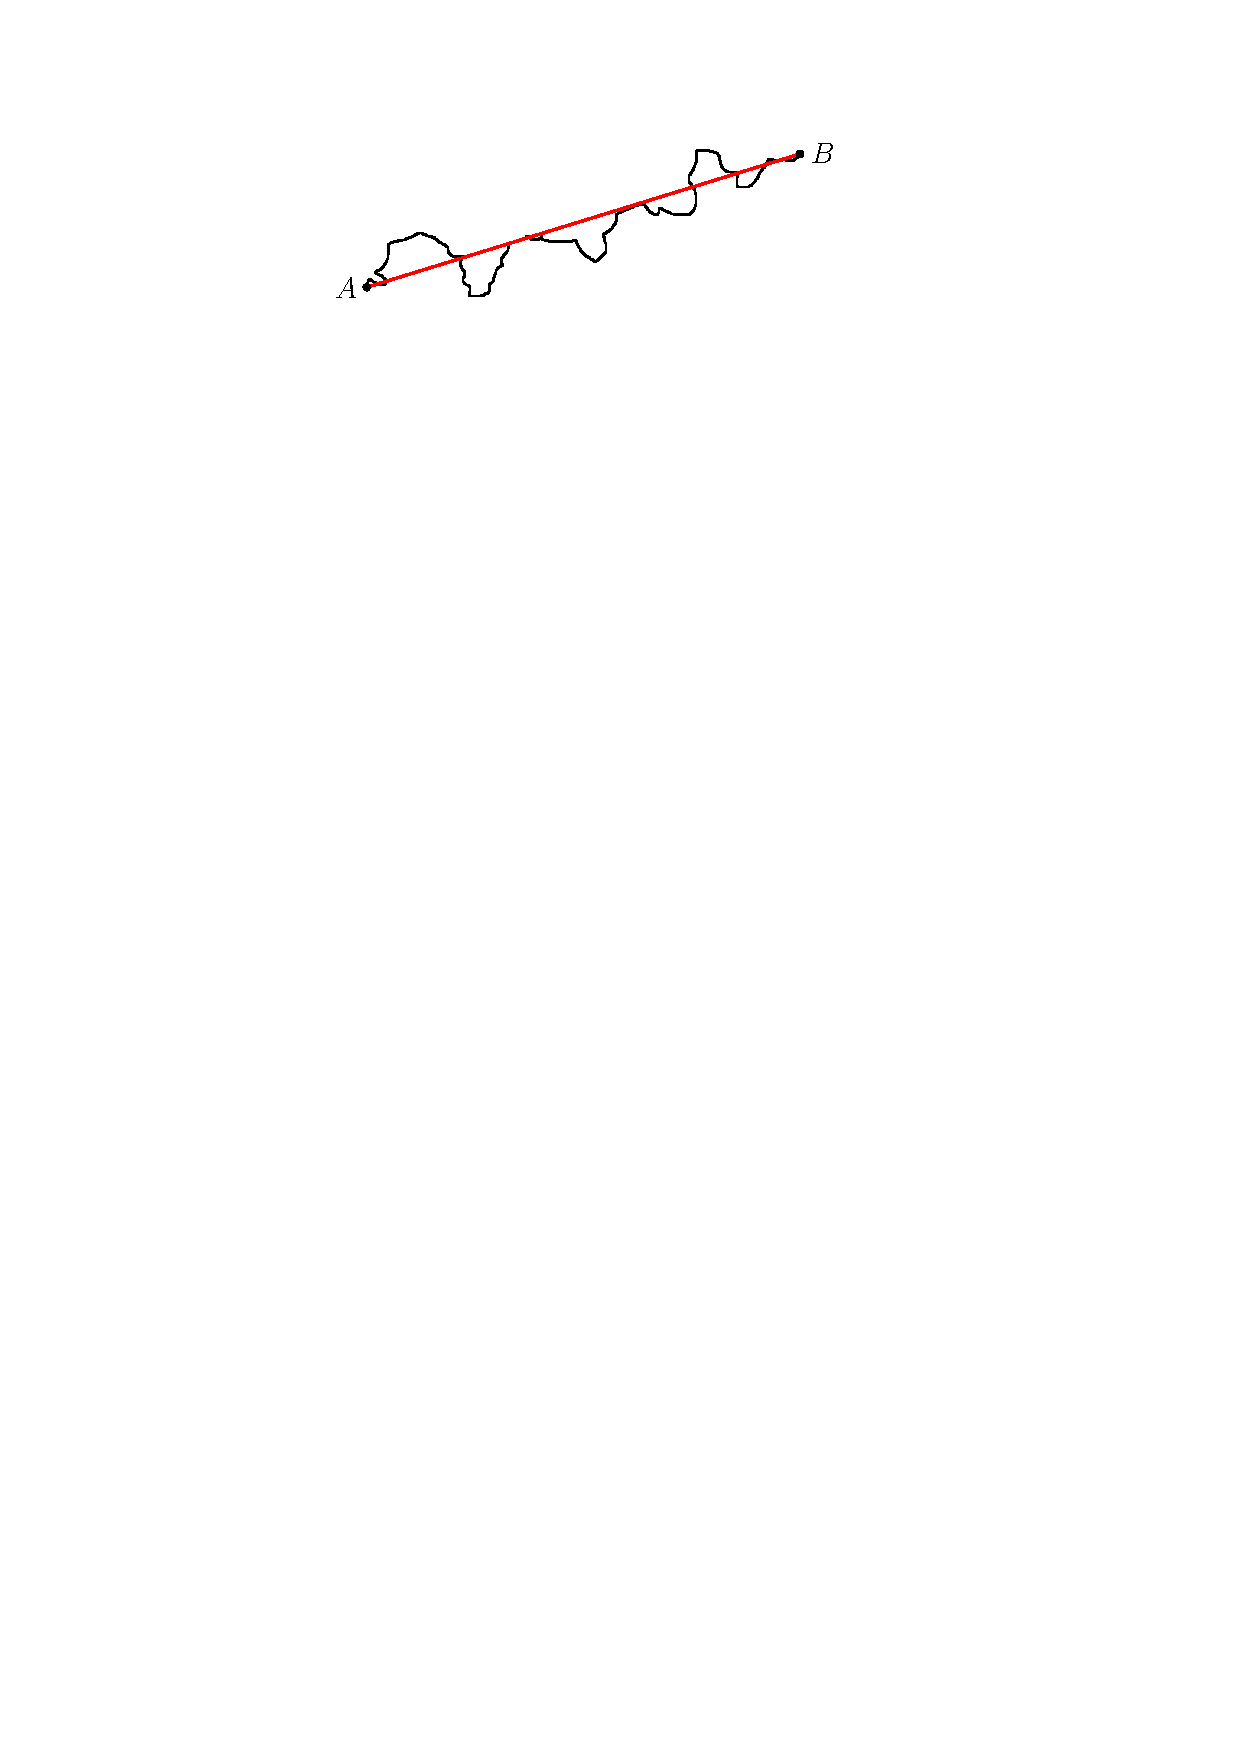
\includegraphics[scale=\normalipe]{ch01-pobrezi.pdf}
    \caption{Příklad mapy pobřeží se spojnicí bodů $A$ a~$B$.}
    \label{fig:pobrezi}
\end{figure}
Zjevně jeho délka je zdola omezena délkou spojnice koncových bodů $A$ a~$B$, nicméně typické pobřeží je velmi nepravidelné a~klikaté. Existují různé metody, které nám umožňují určit jeho délku přesněji. Několik z~nich je popsáno v~knize \citep[str. 79]{Mandelbrot1983}, pro uvedení do problematiky si zde však vystačíme s~tou nejednodušší.\par
Předpokládejme, že pobřeží, které zkoumáme, má pevné hranice (tj. zanedbáváme např. přílivy a~odlivy nastávající během dne), a dále jsme schopni rozlišovat libovolně krátké vzdálenosti.\par
Mějme zadané libovolné $\varepsilon>0$. Podél pobřeží začneme umisťovat tyče tak, že po každém umístění provedeme na mapě krok délky \textbf{nejvýše} $\varepsilon$, přičemž začínáme v~bodě $A$ a~postupujeme až k~bodu $B$ (popř. pokud měříme délku pobřeží ostrova, pokračujeme dokud se nevrátíme tam, kde jsme začali). Předpokládejme, že jsme provedli celkově $n(\varepsilon)$ kroků (jejich počet je závislý na zvolené délce kroku). \emph{Přibližnou délku pobřeží} $\ell(\varepsilon)$ pak stanovíme jako
\begin{equation*}
    \ell(\varepsilon)=n(\varepsilon)\cdot\varepsilon.
\end{equation*}
\begin{figure}[h]
    \centering
    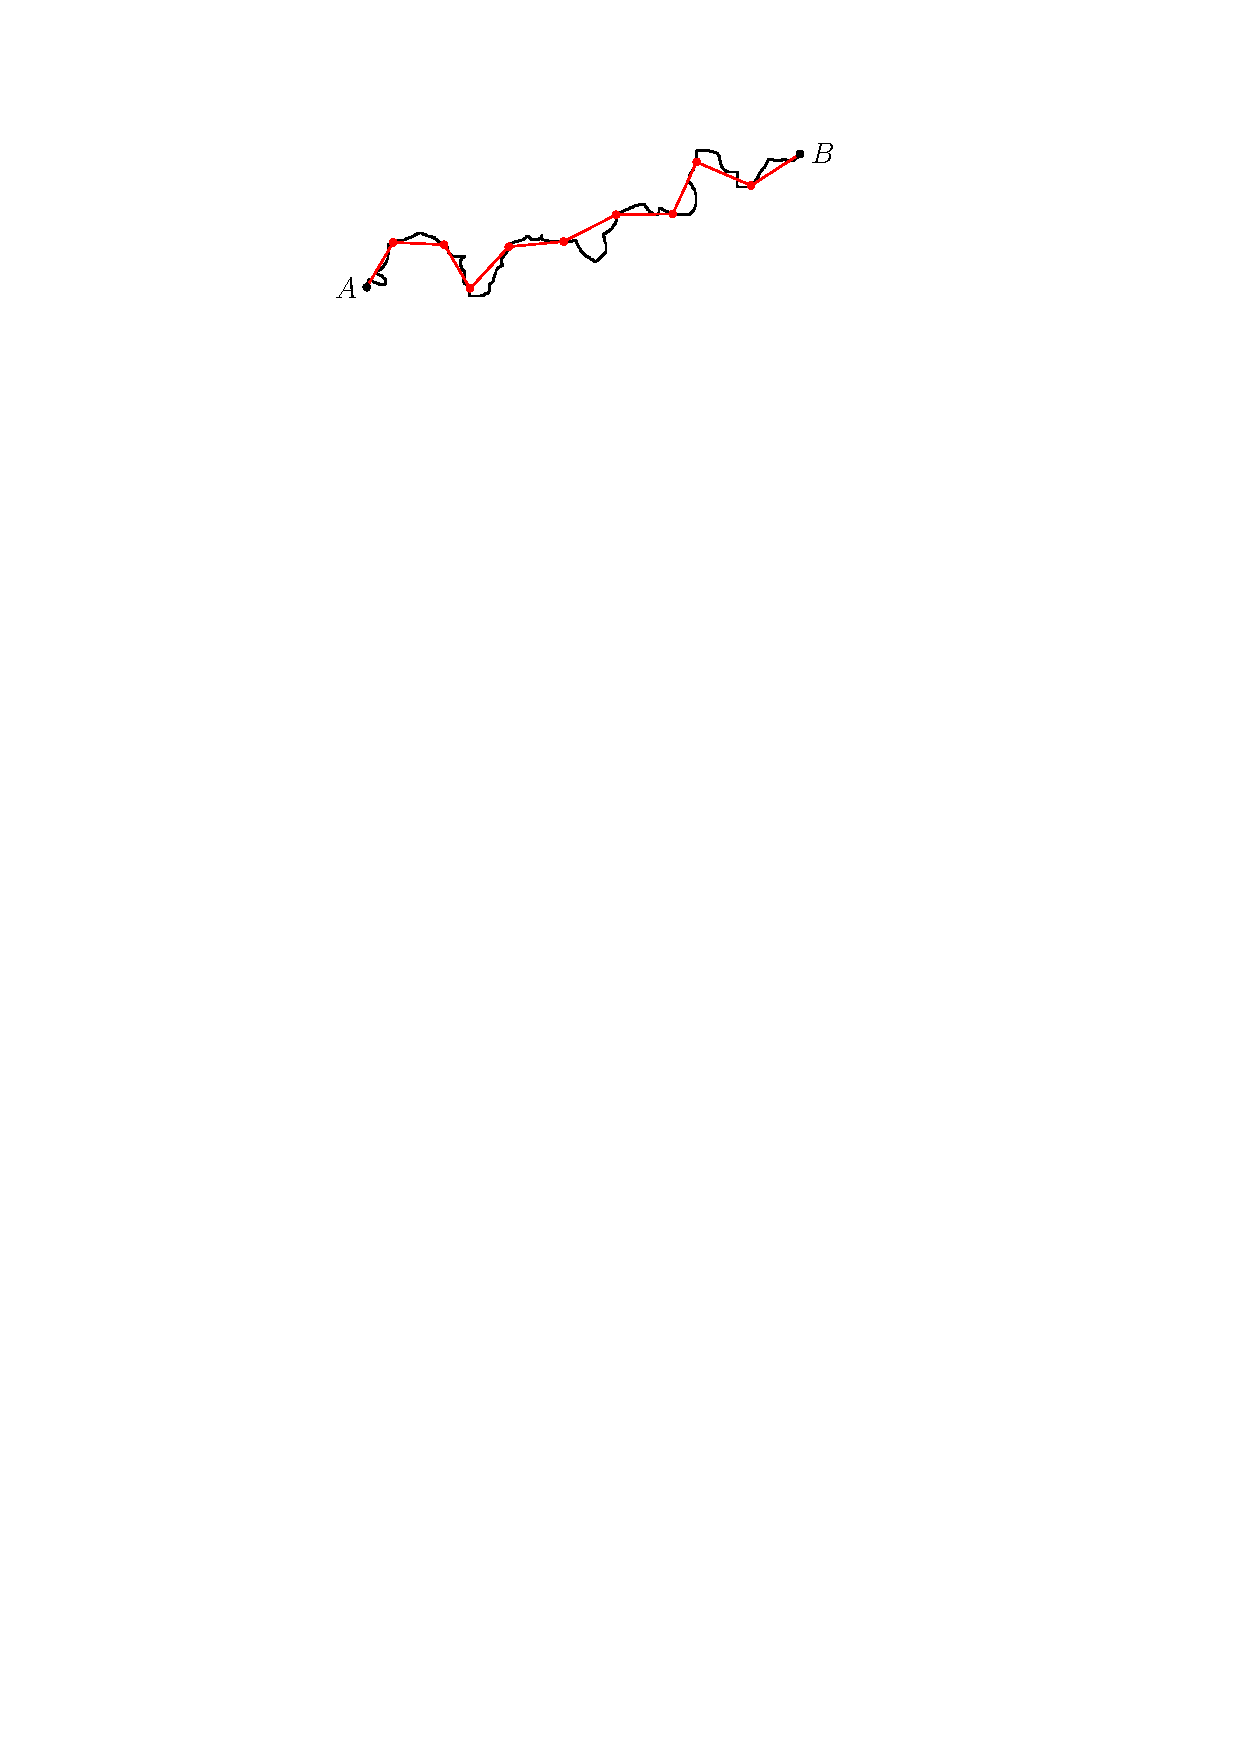
\includegraphics[scale=\normalipe]{ch01-pobrezi-aproximace.pdf}
    \caption{Odhad délky pobřeží, kde $n=10$ při zvoleném $\varepsilon$.}
    \label{fig:pobrezi_aproximace}
\end{figure}
Nyní by nás mohlo napadnout, že pro zmenšující se $\varepsilon$, tj. $\varepsilon\to0_+$, bude hodnota $\ell(\varepsilon)$ konvergovat ke skutečné délce pobřeží. Tzn.~označíme-li skutečnou délku pobřeží $L$, pak bychom mohli očekávat, že platí
\begin{equation}\label{eq:aproximace_limita}
    L=\lim_{\varepsilon\to0_+}{\ell(\varepsilon)}.
\end{equation}
Jenže, bohužel, limita \eqref{eq:aproximace_limita} bude v reálné situaci rovna $\infty$. Proč? Je třeba si uvědomit, že zde pracujeme s~\emph{mapou} pobřeží, která má určité \emph{měřítko}. Pokud bychom měli pobřeží na mapě s~měřítkem $1\,:\,100\;000$, uvidíme méně detailů, než kdybychom jej zkoumali na mapě s~měřítkem $1\,:\,1\;000$. (Viz obrázek~\ref{fig:pobrezi_zoom}.)\par
\begin{figure}[h]
    \centering
    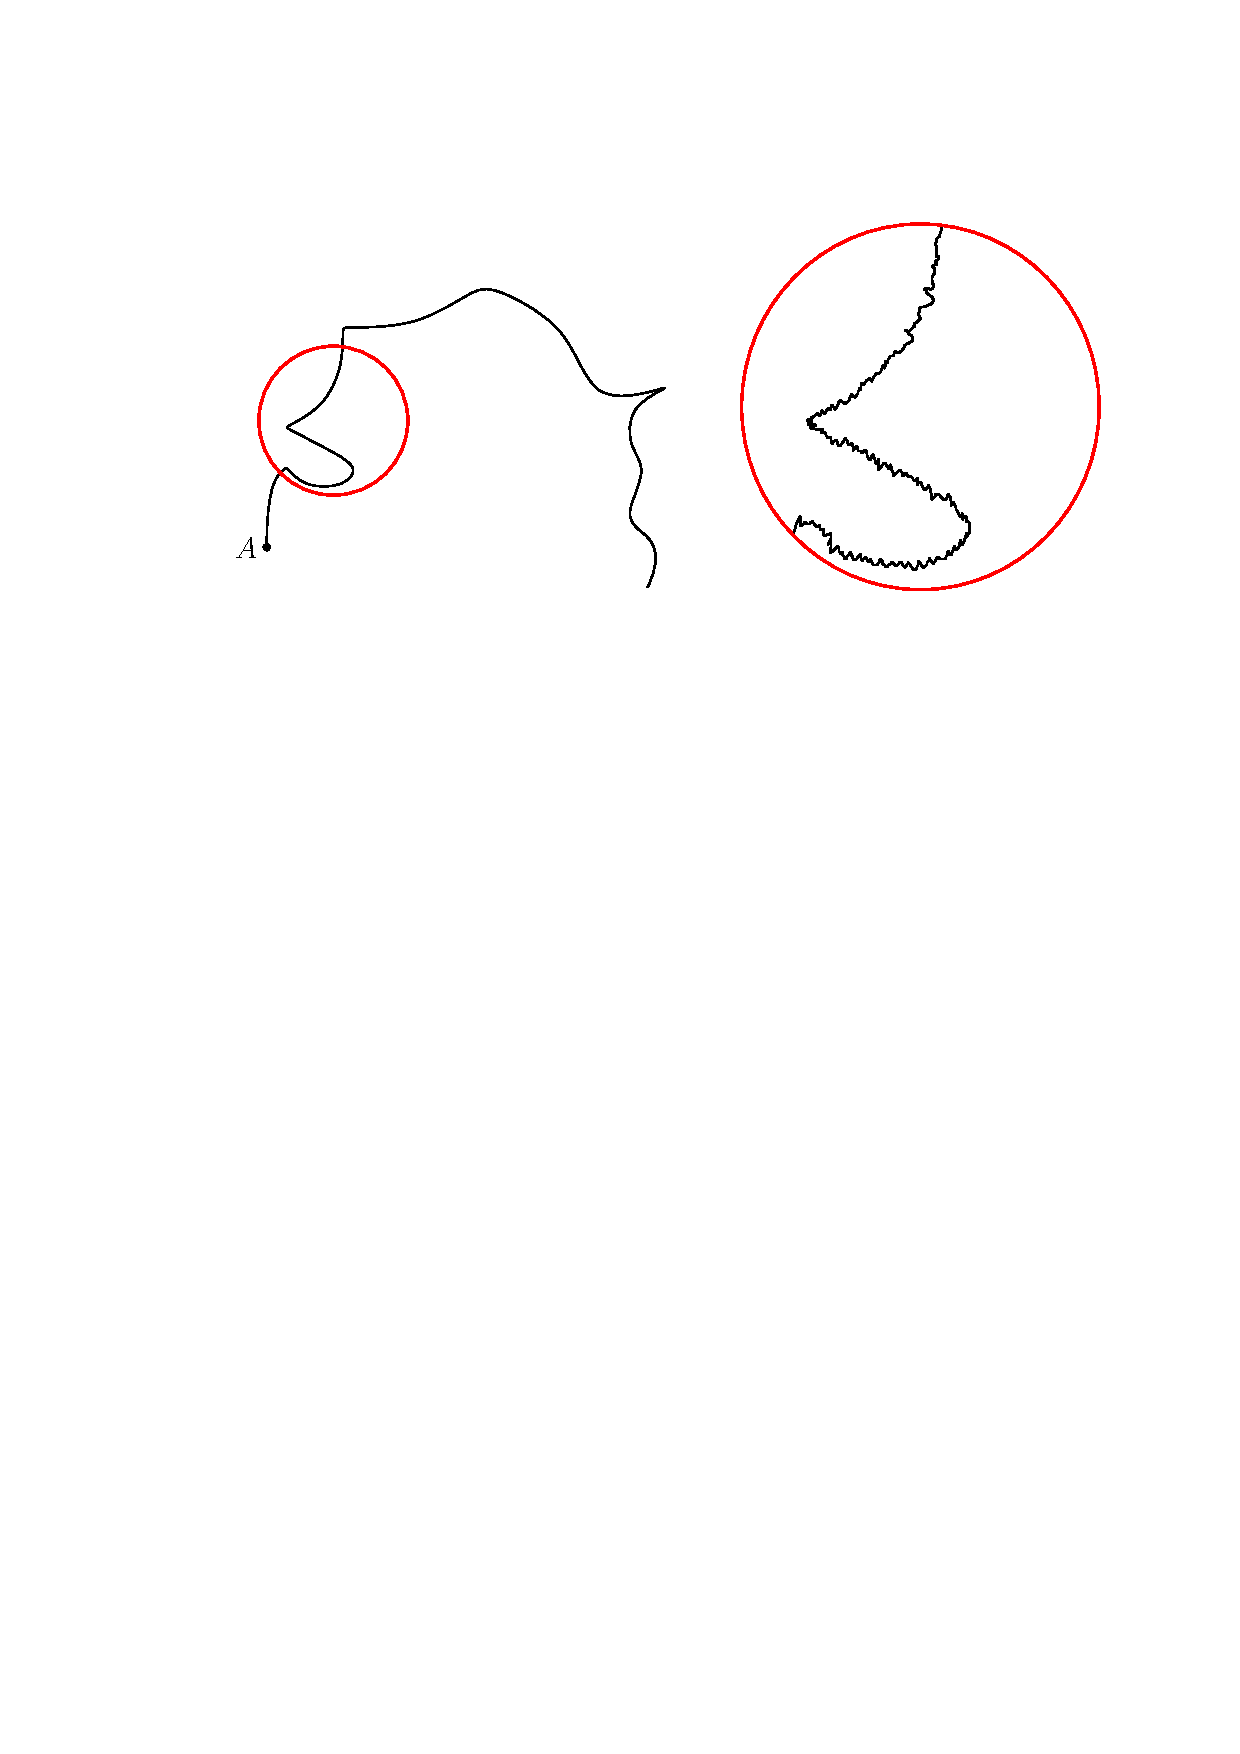
\includegraphics[scale=\normalipe]{ch01-pobrezi-zoom.pdf}
    \caption{Část pobřeží od bodu $A$ v~menším měřítku.}
    \label{fig:pobrezi_zoom}
\end{figure}
Nově odhalené detaily (menší poloostrůvky apod.) zde přispívají k~celkové délce pobřeží $\ell(\varepsilon)$. Postupným zvětšováním měřítka mapy bychom tak odhalili další detaily. Naše původní idea tak selhává, neboť (v "klasickém" pojetí délky) pro $\varepsilon\to0_+$ hodnota $\ell(\varepsilon)$ patrně poroste nade všechny meze, tj. $\lim_{\varepsilon\to0_+}{\ell(\varepsilon)}=\infty$.\par
Nabízí se otázka: Proč se toto děje? Pokud se ohlédneme zpět za eukleidovskou geometrií\index{geometrie!eukleidovská}\index{eukleidovská geometrie}, tento problém v ní nenastává. Např. u~kružnice v~eukleidovské rovině $\mathbb{E}_2$ změnou měřítka žádné další detaily křivky neobjevíme (podobně u~jiných geometrických útvarů, viz obrázky~\ref{subfig:kruznice} a~\ref{subfig:kruznice_zoom}). 
\begin{figure}[h]
    \centering
    \begin{subfigure}{\subfigwidth}
        \centering
        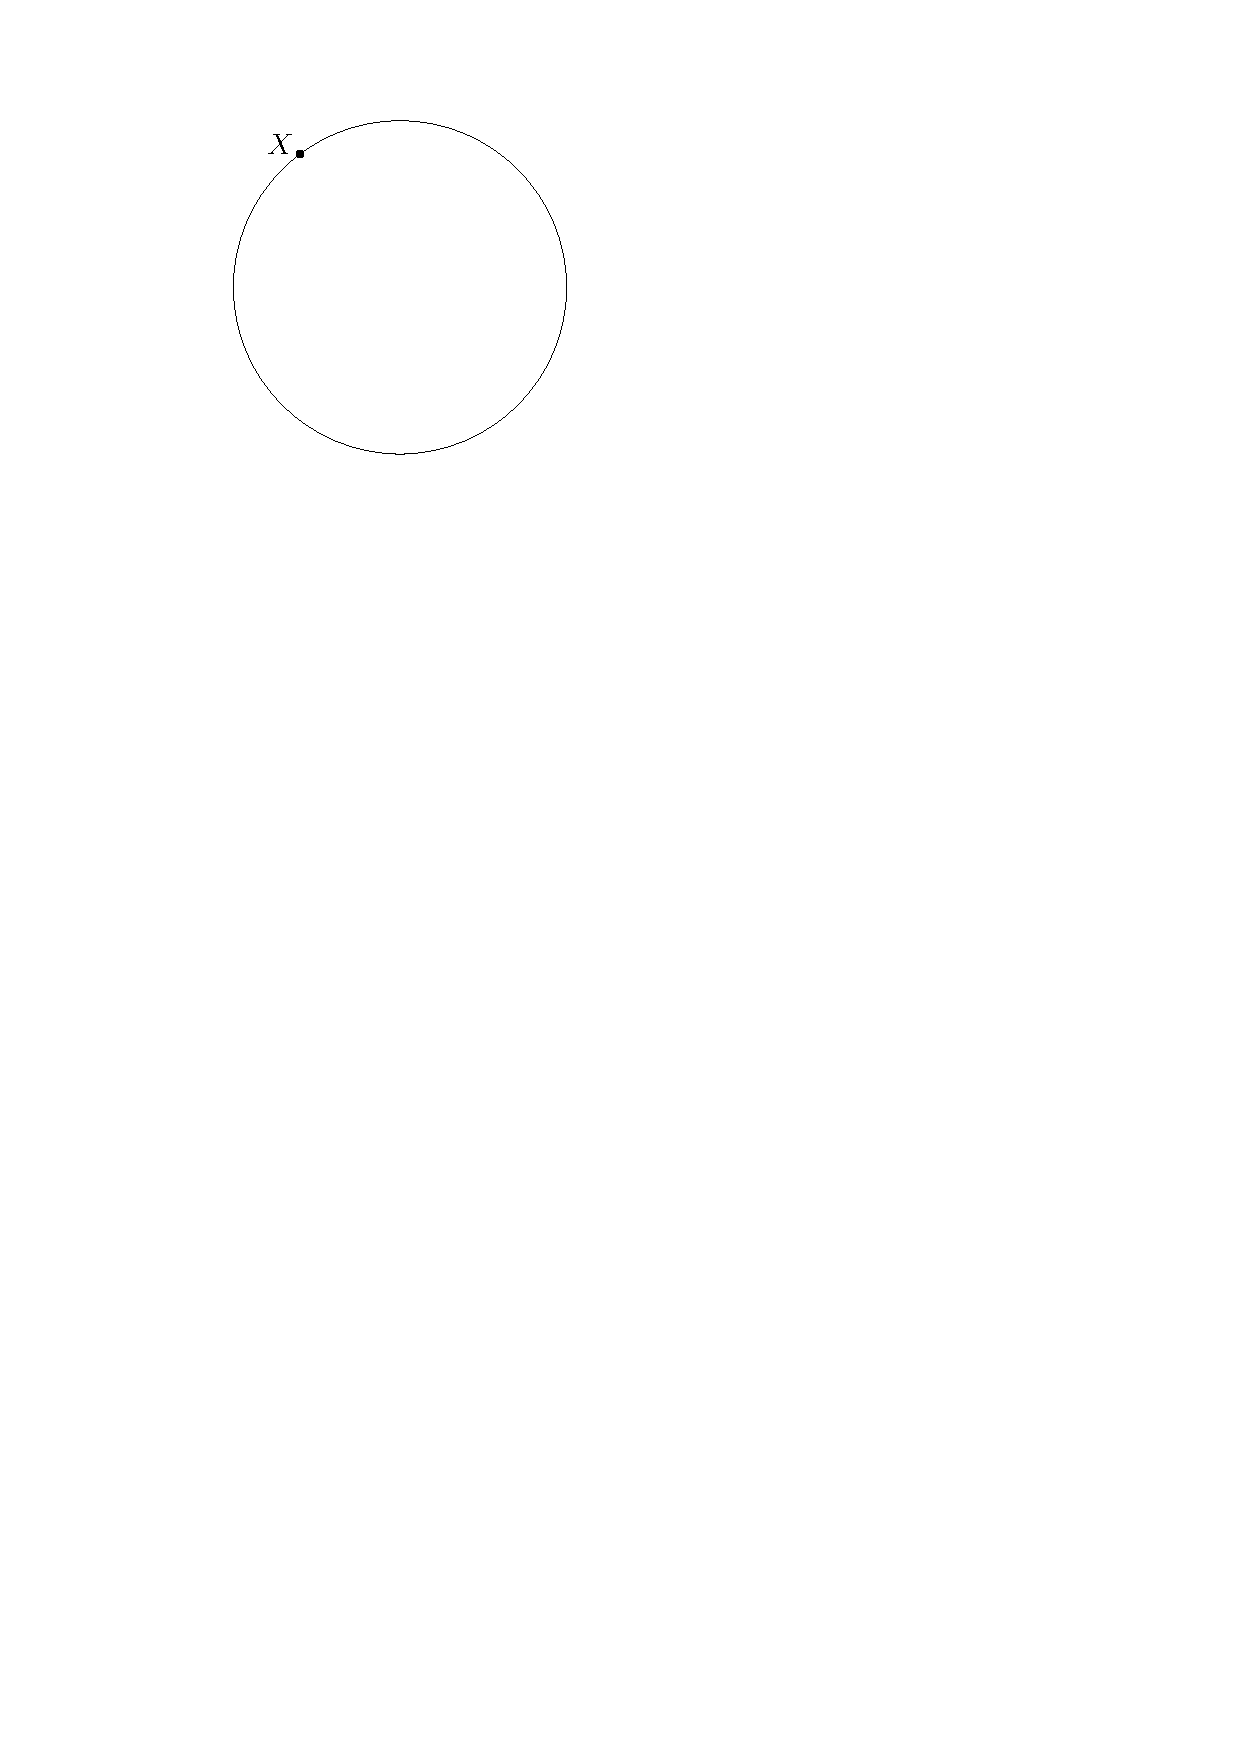
\includegraphics[scale=\normalipe]{ch01-kruznice.pdf}
        \caption{Kružnice v~menším měřítku.}
        \label{subfig:kruznice}
    \end{subfigure}
    \quad
    \begin{subfigure}{\subfigwidth}
        \centering
        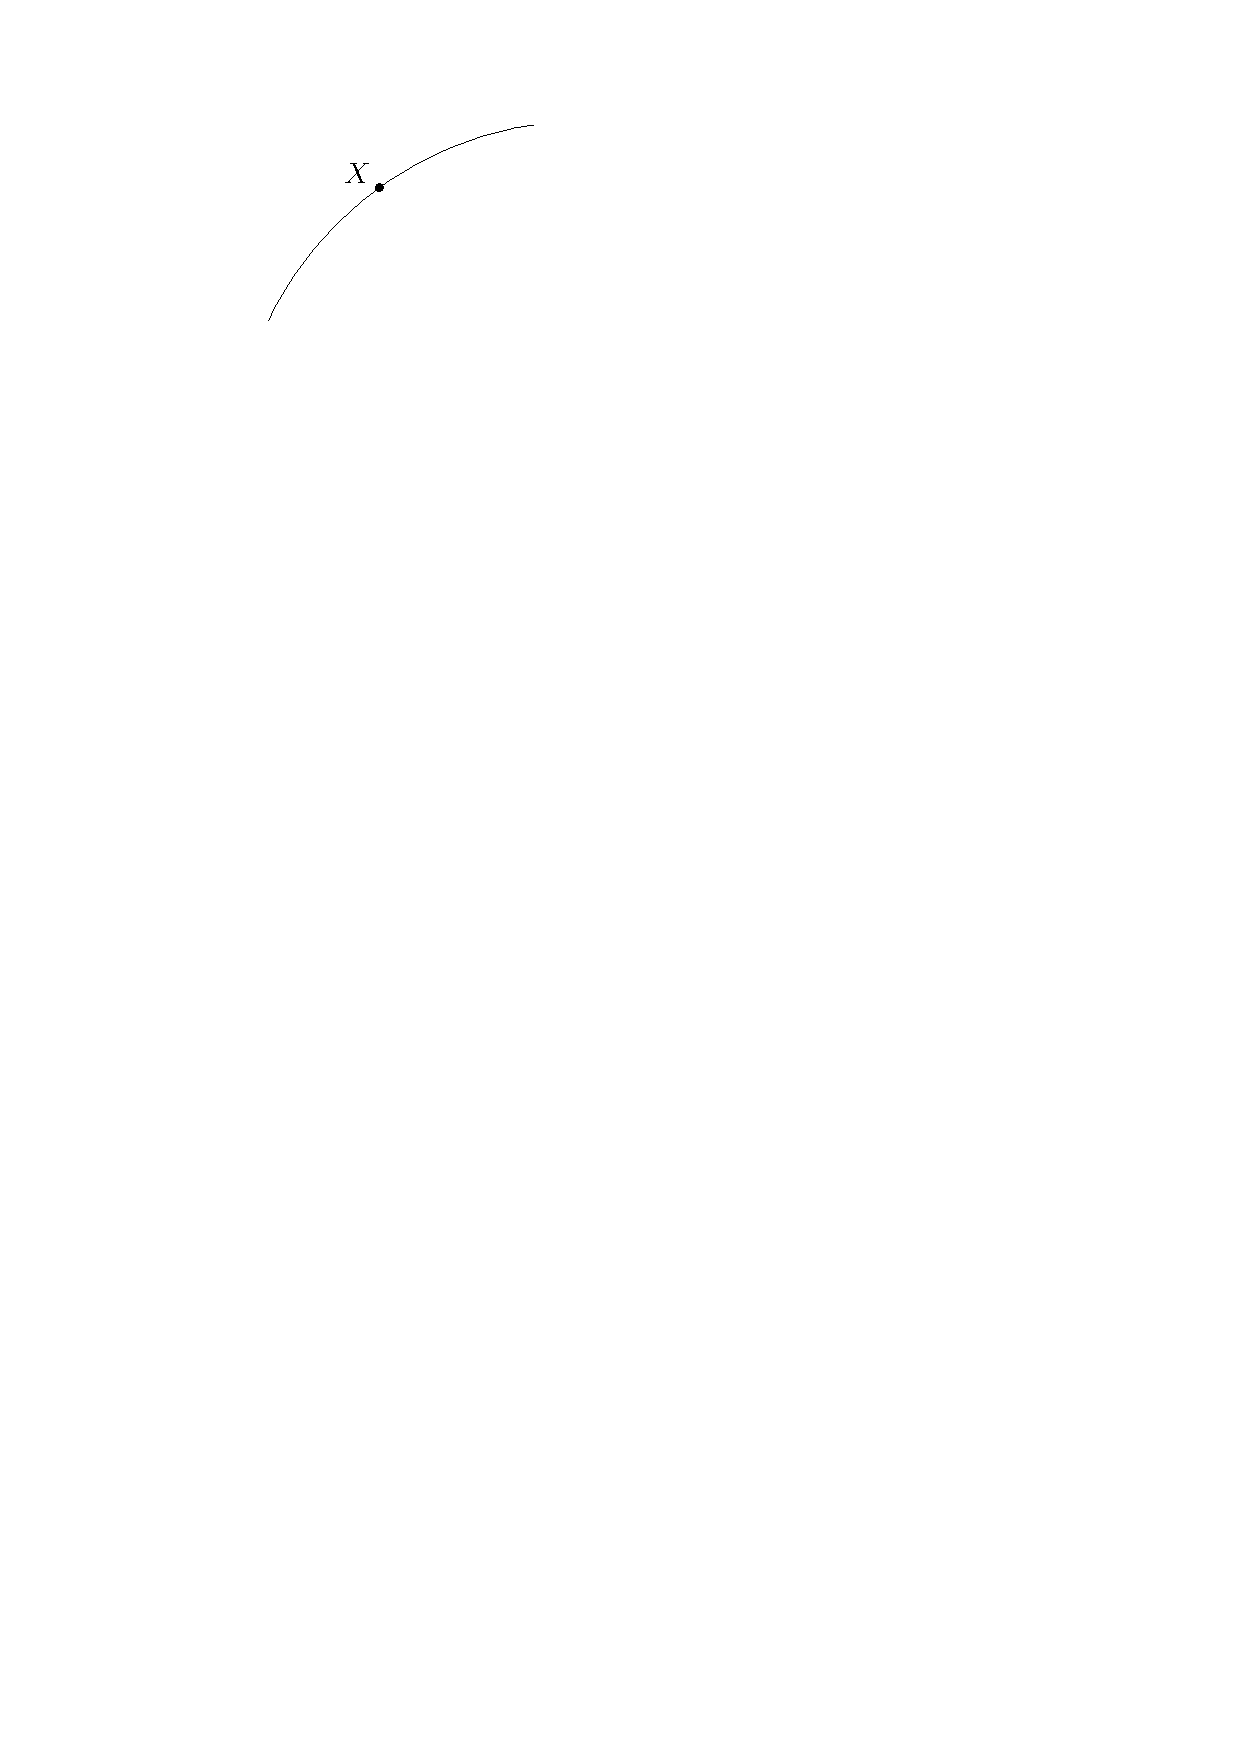
\includegraphics[scale=\normalipe]{ch01-kruznice-zoom.pdf}
        \caption{Část kružnice ve větším měřítku.}
        \label{subfig:kruznice_zoom}
    \end{subfigure}
\end{figure}
Díky tomu můžeme v~případě počítání obvodu kružnice použít následující postup.\par
Máme-li kružnici o~poloměru $r>0$, pak jí můžeme vepsat libovolný pravidelný $n$-úhelník (viz obrázek~\ref{subfig:archimedova_metoda}).
\begin{figure}[h]
    \centering
    \begin{subfigure}{\subfigwidth}
        \centering
        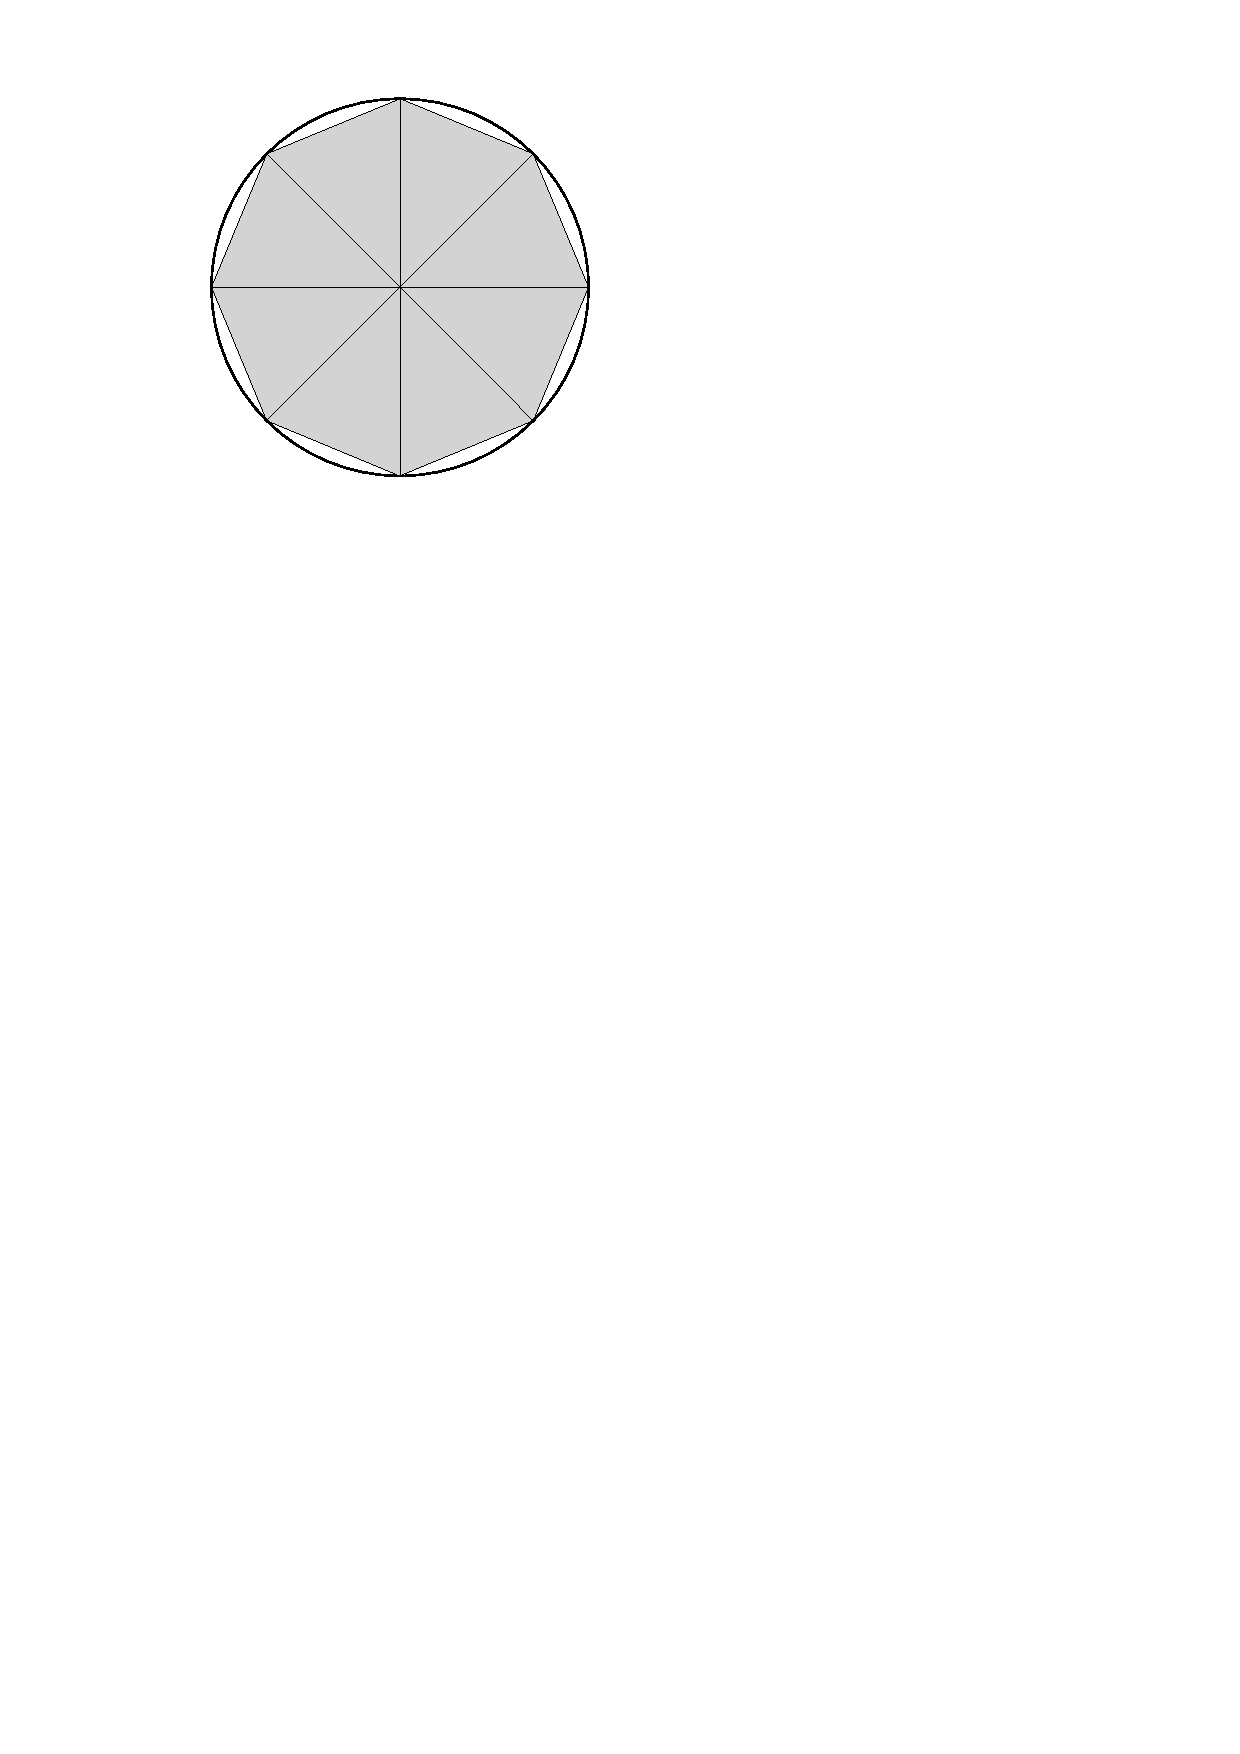
\includegraphics[scale=\normalipe]{ch01-archimedova-metoda.pdf}
        \caption{Pravidelný osmiúhelník vepsaný kružnici.}
        \label{subfig:archimedova_metoda}
    \end{subfigure}
    \quad
    \begin{subfigure}{\subfigwidth}
        \centering
        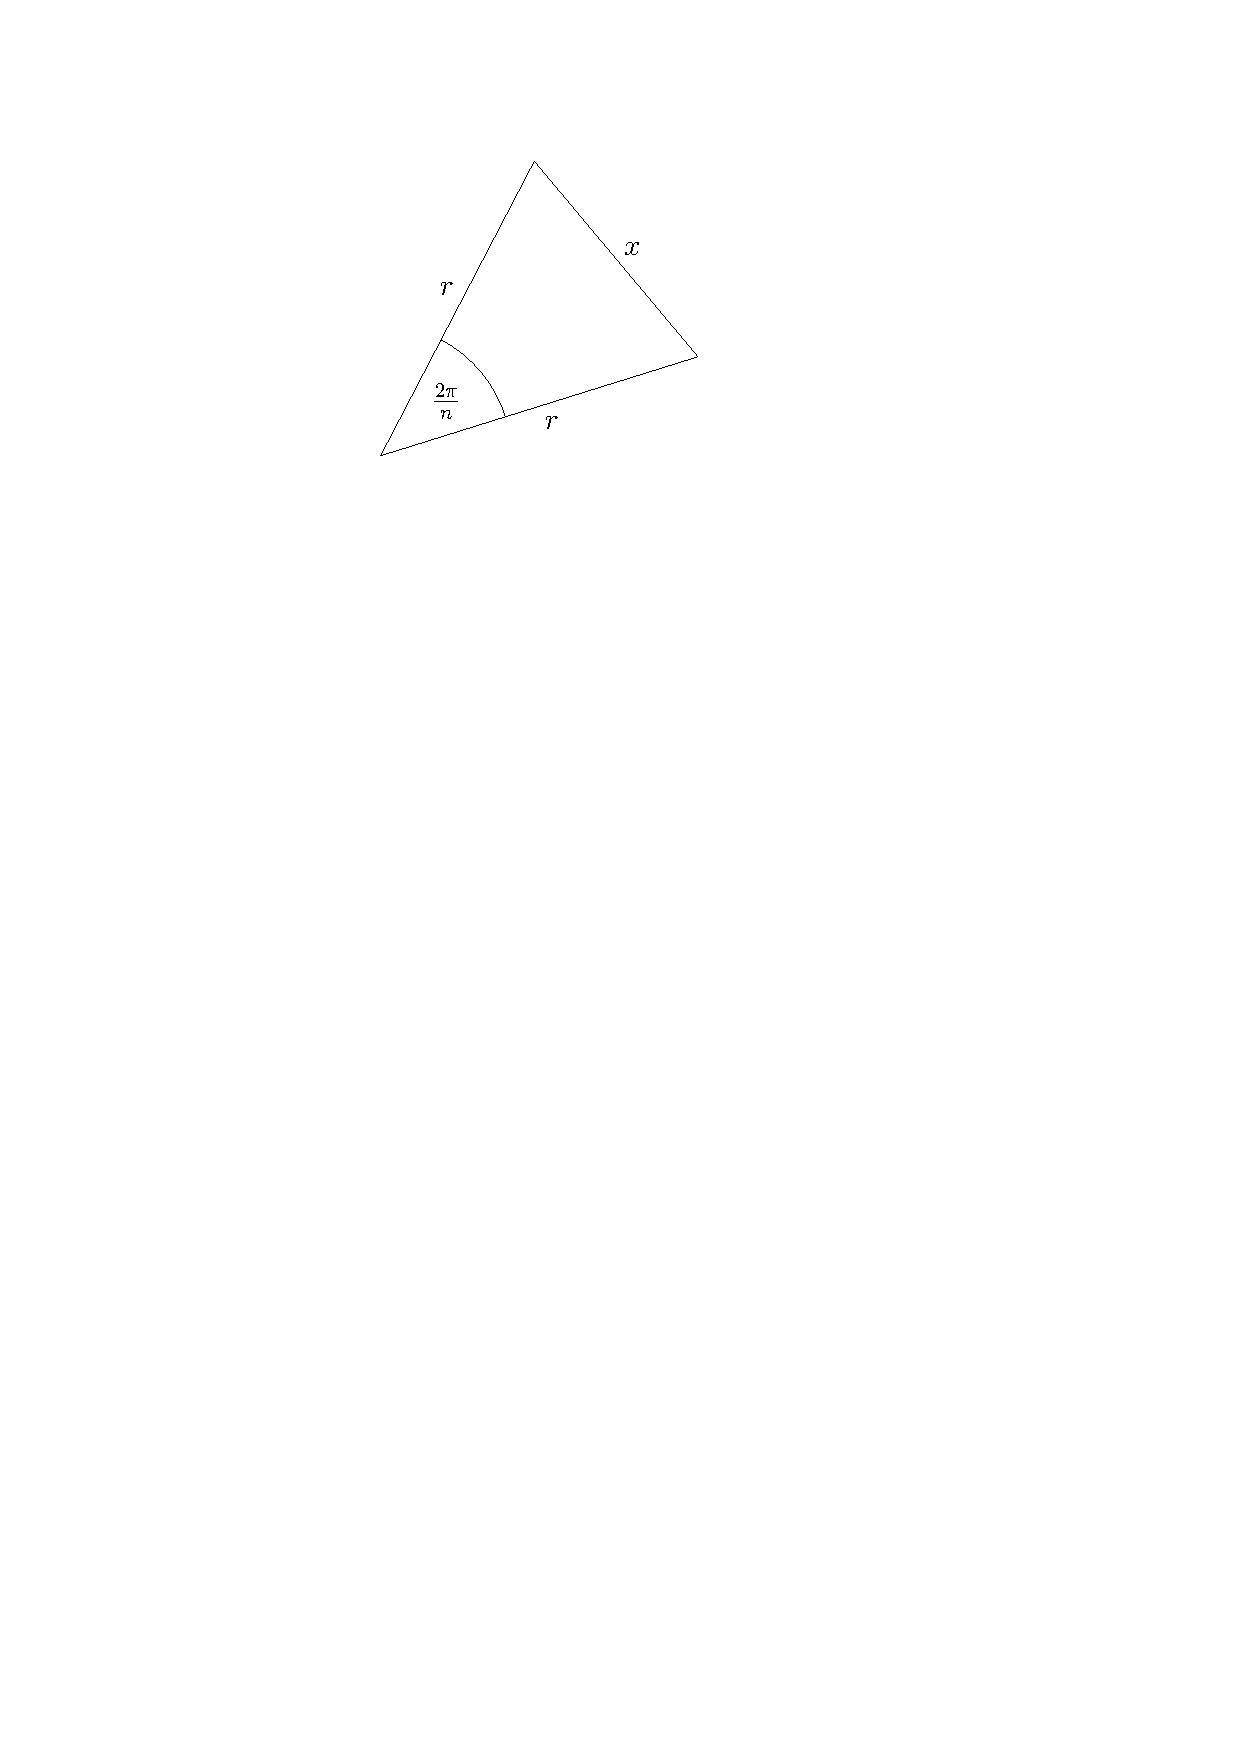
\includegraphics[scale=\normalipe]{ch01-archimedova-metoda-cast-nuhelniku.pdf}
        \caption{Část vepsaného pravidelného $n$-úhelníku.}
        \label{subfig:archimedova_metoda_cast_nuhelniku}
    \end{subfigure}
    \caption{Princip Archimédovy metody.}
    \label{fig:princip_archimedovy_metody}
\end{figure}
Obvod pravidelného $n$-úhelníku is označíme $O_n$ a~délku jeho strany $x$ (viz obrázek~\ref{subfig:archimedova_metoda_cast_nuhelniku}). Tu jsme schopni stanovit užitím elementární goniometrie, tj.
\begin{equation*}
    x=2r\cdot\sin{\dfrac{\pi}{n}},
\end{equation*}
a tedy obvod
\begin{equation*}
    O_n=2rn\cdot\sin{\dfrac{\pi}{n}}.
\end{equation*}
Pro rostoucí $n$ bude obvod pravidelného $n$-úhelníku stále lépe aproximovat obvod původní kružnice (viz obrázek~\ref{fig:archimedova_metoda_presnejsi}).
\begin{figure}[h]
    \centering
    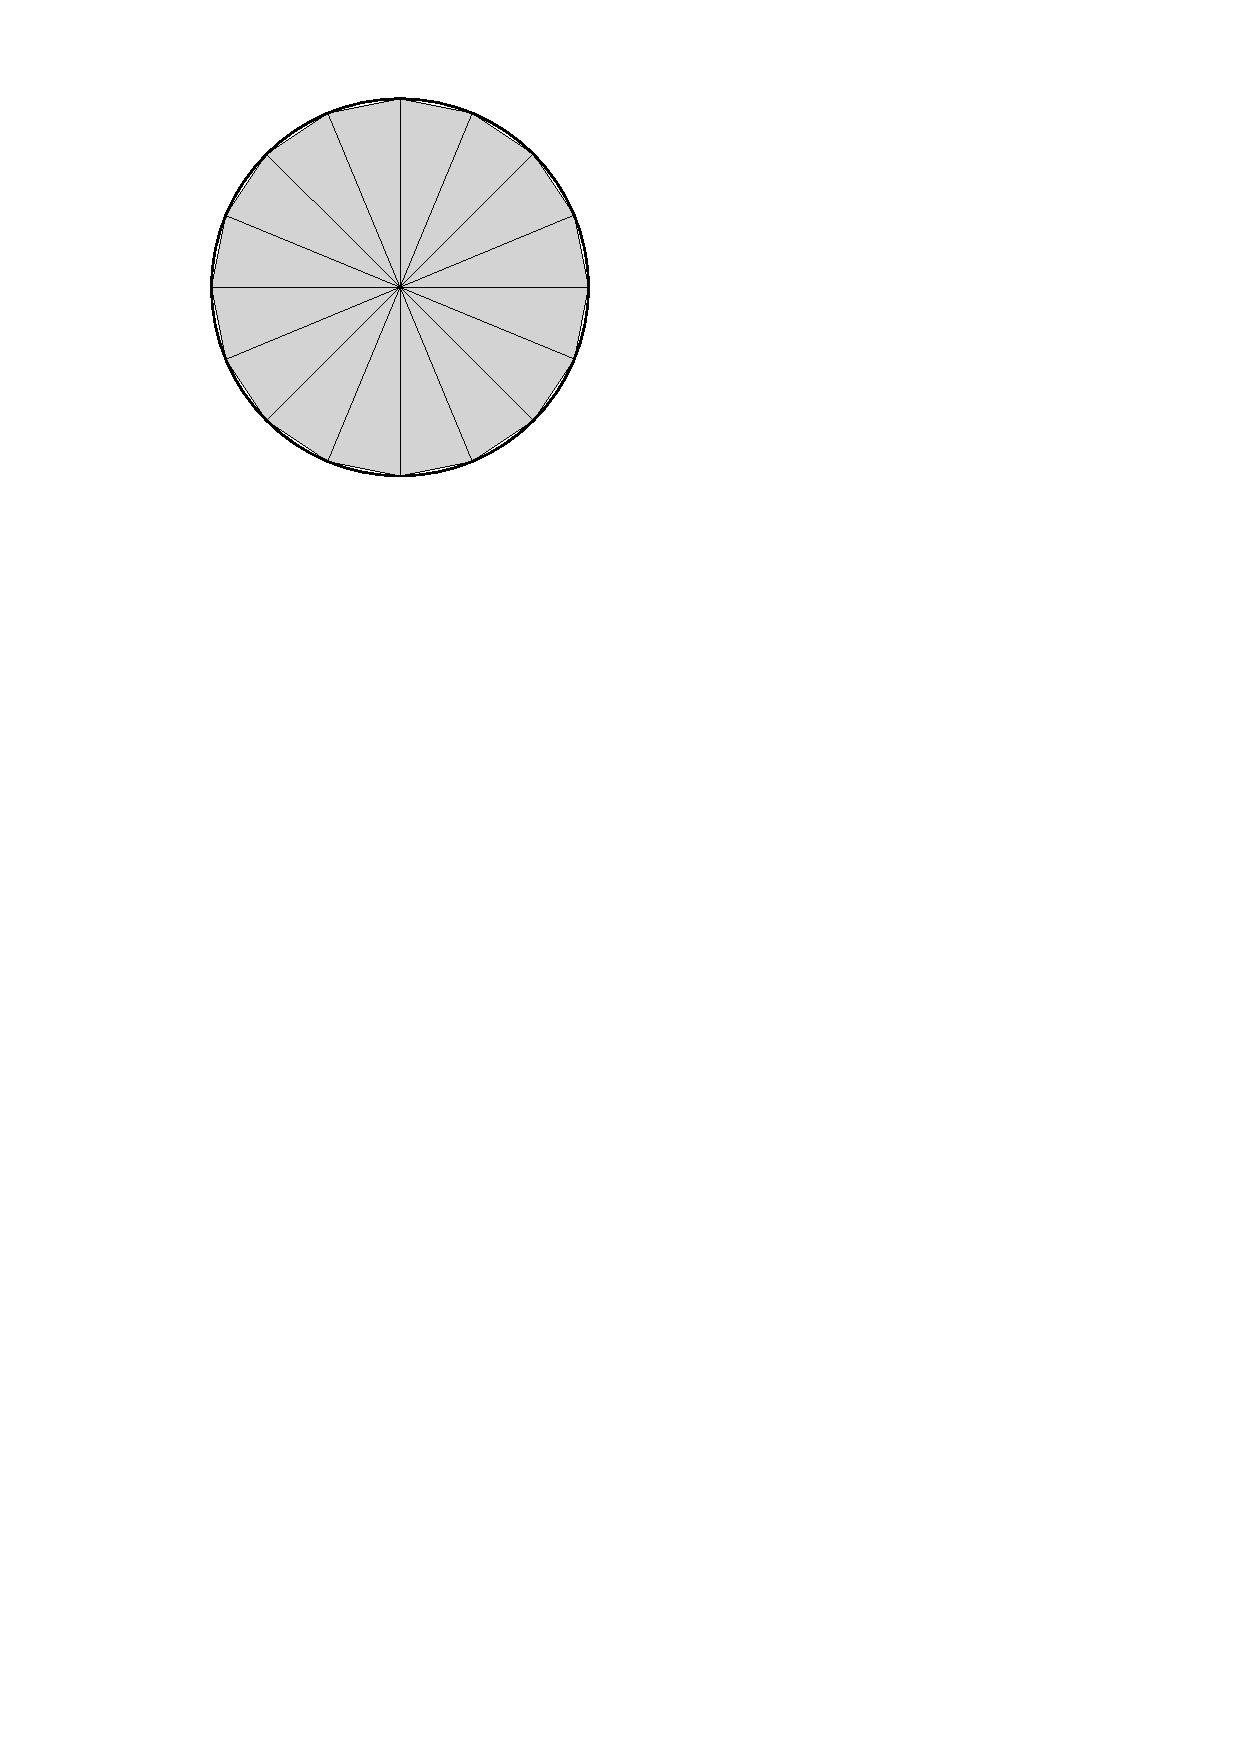
\includegraphics[scale=\normalipe]{ch01-pobrezi-aproximace-presnejsi.pdf}
    \caption{Aproximace obvodu kružnice pomocí pravidelného šestnáctiúhelníku.}
    \label{fig:archimedova_metoda_presnejsi}
\end{figure}
Limitním přechodem (tj. pro $n\to\infty$) tak můžeme odvodit vzorec pro obvod kružnice:
\begin{align*}
    O&=\lim_{n\to\infty}{2rn\cdot\sin{\dfrac{\pi}{n}}}=2r\cdot\lim_{n\to\infty}{n\cdot\sin{\dfrac{\pi}{n}}}=2\pi r\cdot\lim_{n\to\infty}{\cdot\dfrac{\sin{\dfrac{\pi}{n}}}{\dfrac{\pi}{n}}}=2\pi r.
\end{align*}
Idea aproximace pomocí "zjemňování" zde skutečně funguje a~délka ve standardním pojetí tak dává smysl, jak bychom mohli očekávat. Křivka, kterou tvoří pobřeží, má však oproti kružnici jiný geometrický charakter. Délka pobřeží $\infty$, k~níž Mandelbrot došel, tak dává smysl \emph{z geometrického pohledu}, avšak výsledek to není moc užitečný.
\section{Soběpodobnost}\label{sec:sobepodobnost}
Mandelbrot si uvědomil,~že struktura pobřeží se charakterově vymyká útvarům do tehdy známým eukleidovské geometrii,~neboť mapy s~různými měřítky poskytovaly různou úroveň detailů,~které hrály netriviální roli v~jeho celkové délce. Učinil však jiné zásadní pozorování,~a to sice,~že mnoho detailů má společné rysy,~které se opakují. Hodně z~nich se shodovalo s~výjimkou jejich měřítka. \citep[str. 96]{Mandelbrot1983}\par

Ve fraktální geometrii se pro tento úkaz uchytil termín \emph{soběpodobnost} (angl. \emph{self-similarity}). Útvar nazýváme soběpodobným,~\textbf{pokud se sám sobě podobný v~libovolném měřítku} \citep[str. 220]{Voracova2022} nebo pokud \textbf{část útvaru je podobná jeho celku}. Zmíněná podoba může být míněna přibližně (např. v~případě pobřeží je nejspíše jasné,~že žádné z~jeho detailů nesdílejí společné rysy přesně),~ale v~dalších částech si předvedeme soběpodobnost \emph{přímou}\index{soběpodobnost}.

\subsection{Kochova křivka}\label{subsec:kochova_krivka}
Jak jsme si již uvedli,~za otce fraktální geometrie je považován Mandelbrot,~avšak mnoho fraktálních křivek bylo známo již dříve (čtenář promine,~že jsme blíže nespecifikovali termín "fraktální",~jeho přesný význam pro nás však zatím nebude stěžejní). Jako první se podíváme na jednu z~nejznámějších,~kterou objevil roku \emph{1904} švédský matematik \name{Helge~von~Koch} \mbox{(1870--1924)},~dnes známou pod~názvem \emph{Kochova křivka}\index{Kochova křivka}\index{křivka!Kochova}. \citep[str. 61]{Peitgen2004} Na začátku vezmeme úsečku délky $1$. Vyjmeme prostřední (tj. druhou) třetinu a nahradíme ji dvěma úsečkami délky $1/3$,~tak,~aby na sebe navazovaly v~krajních bodech. Tento proces následně opakujeme pro nově vzniklé úsečky. Obecně u~úsečky délky $l$ nahradíme její prostřední třetinu dvojicí úseček délek $l/3$ (viz obrázek \ref{fig:kochova_vlocka_5iteraci}).
\begin{figure}[h]
    \centering
    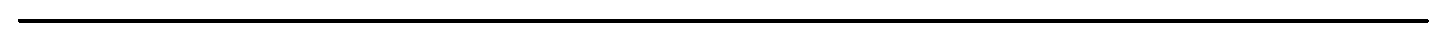
\includegraphics[scale=\fractalscale]{ch01-kochova-krivka-0iterace.pdf}\\\qquad\\
    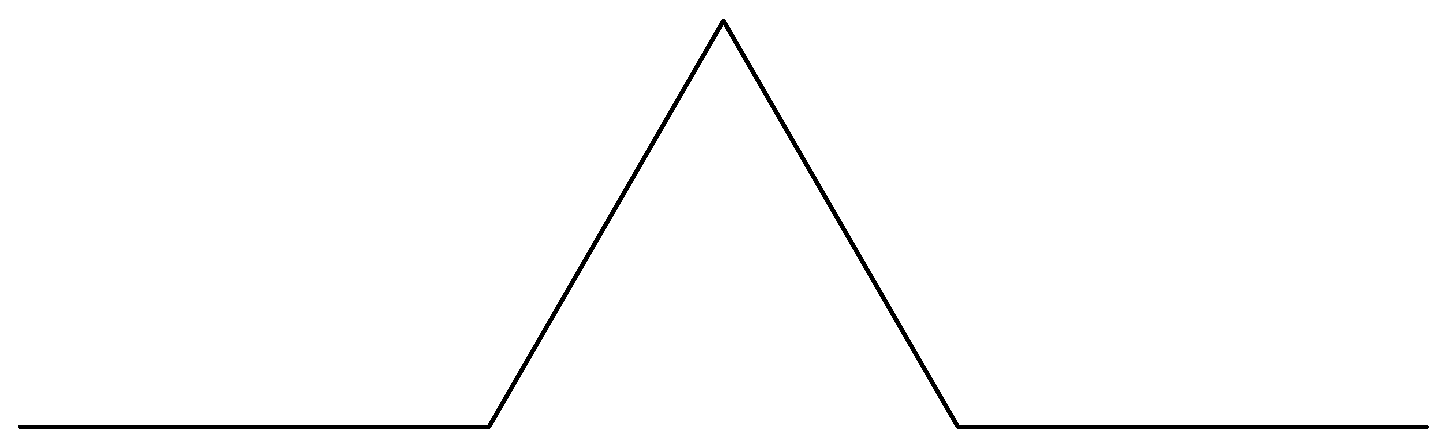
\includegraphics[scale=\fractalscale]{ch01-kochova-krivka-1iterace.pdf}\\\qquad\\
    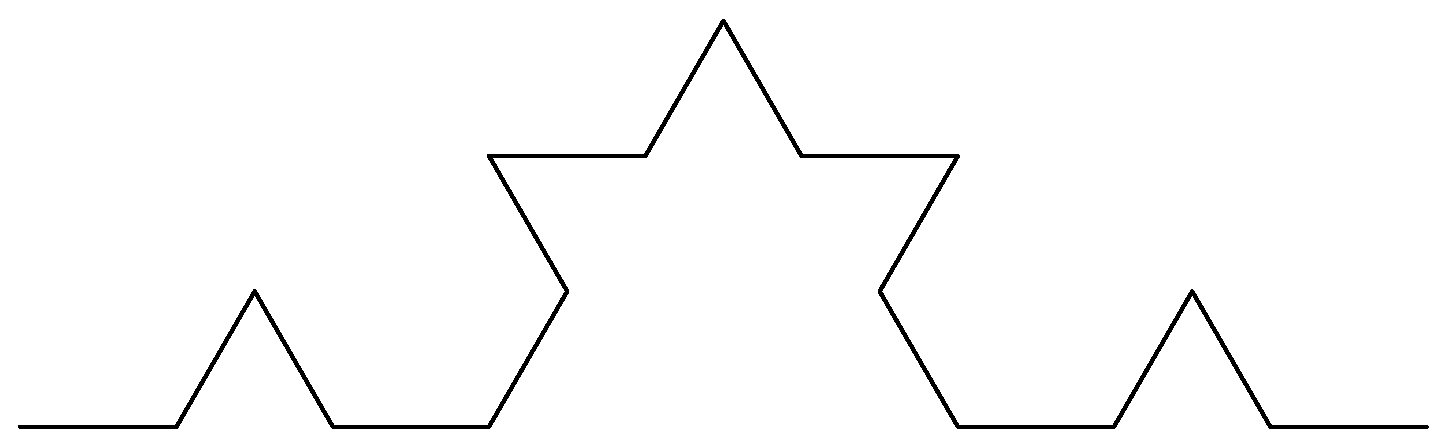
\includegraphics[scale=\fractalscale]{ch01-kochova-krivka-2iterace.pdf}\\\qquad\\
    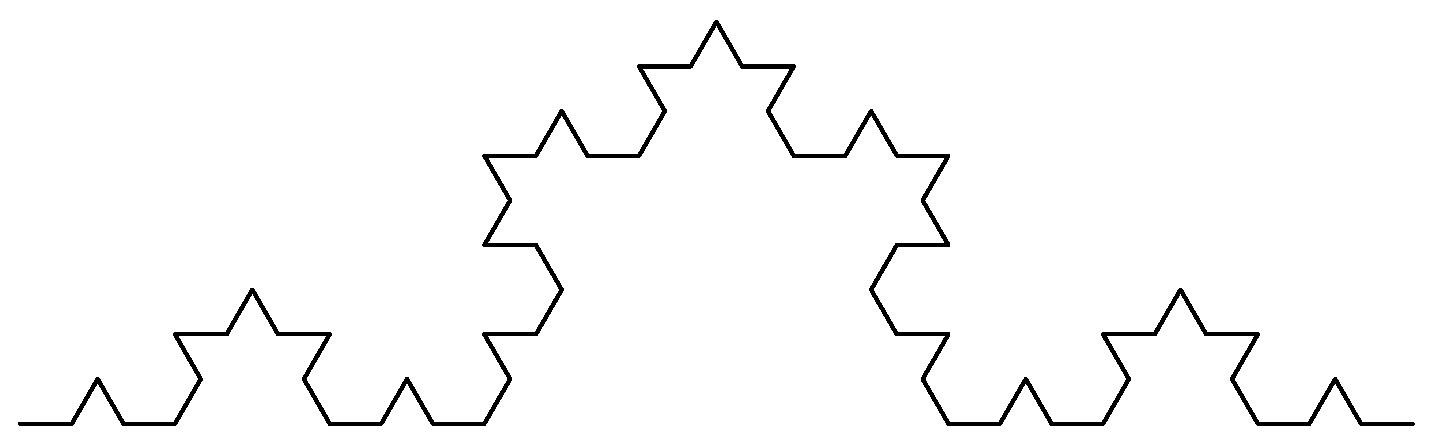
\includegraphics[scale=\fractalscale]{ch01-kochova-krivka-3iterace.pdf}\\\qquad\\
    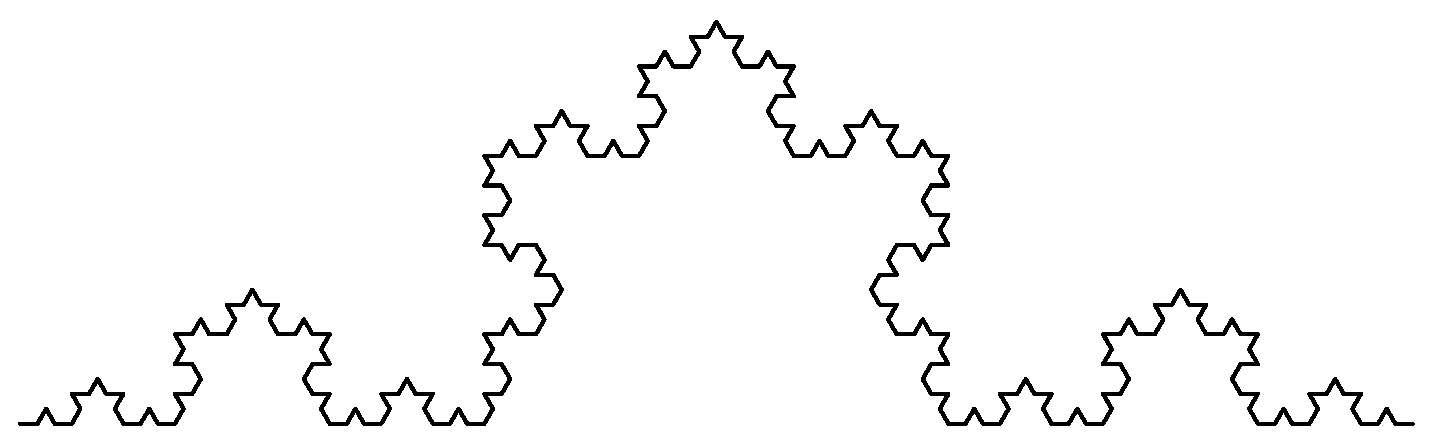
\includegraphics[scale=\fractalscale]{ch01-kochova-krivka-4iterace.pdf}\\\qquad\\
    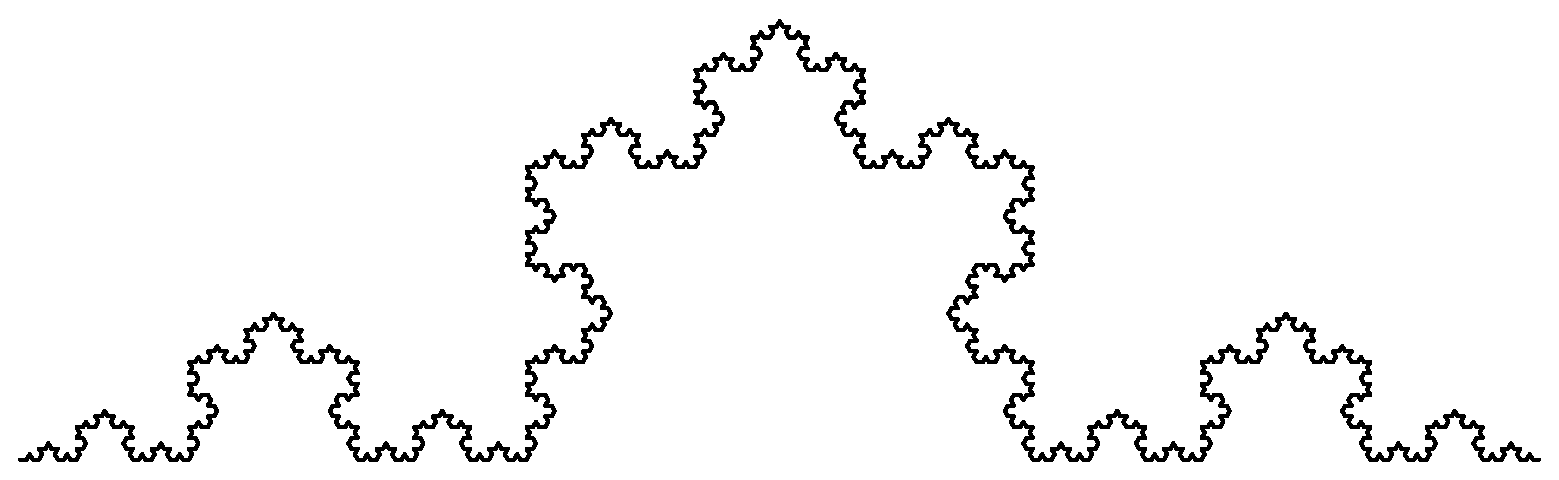
\includegraphics[scale=\fractalscale]{ch01-kochova-krivka-5iterace.pdf}
    \caption{Prvních pět iterací Kochovy křivky.}
    \label{fig:kochova_vlocka_5iteraci}
\end{figure}
V první řadě si můžeme všimnout,~že v~každé další iteraci jsou nově vzniklé podobné původnímu celku,~tedy v~předešlé iteraci (viz obrázek \ref{fig:kochova_krivka_podobnost}). Pokud by tento proces pokračoval do nekonečna,~pak by každá ze čtyř částí křivky představovala \textbf{celý původní obrazec} ve zmenšeném měřítku (byla by tedy soběpodobná).
\begin{figure}[h]
    \centering
    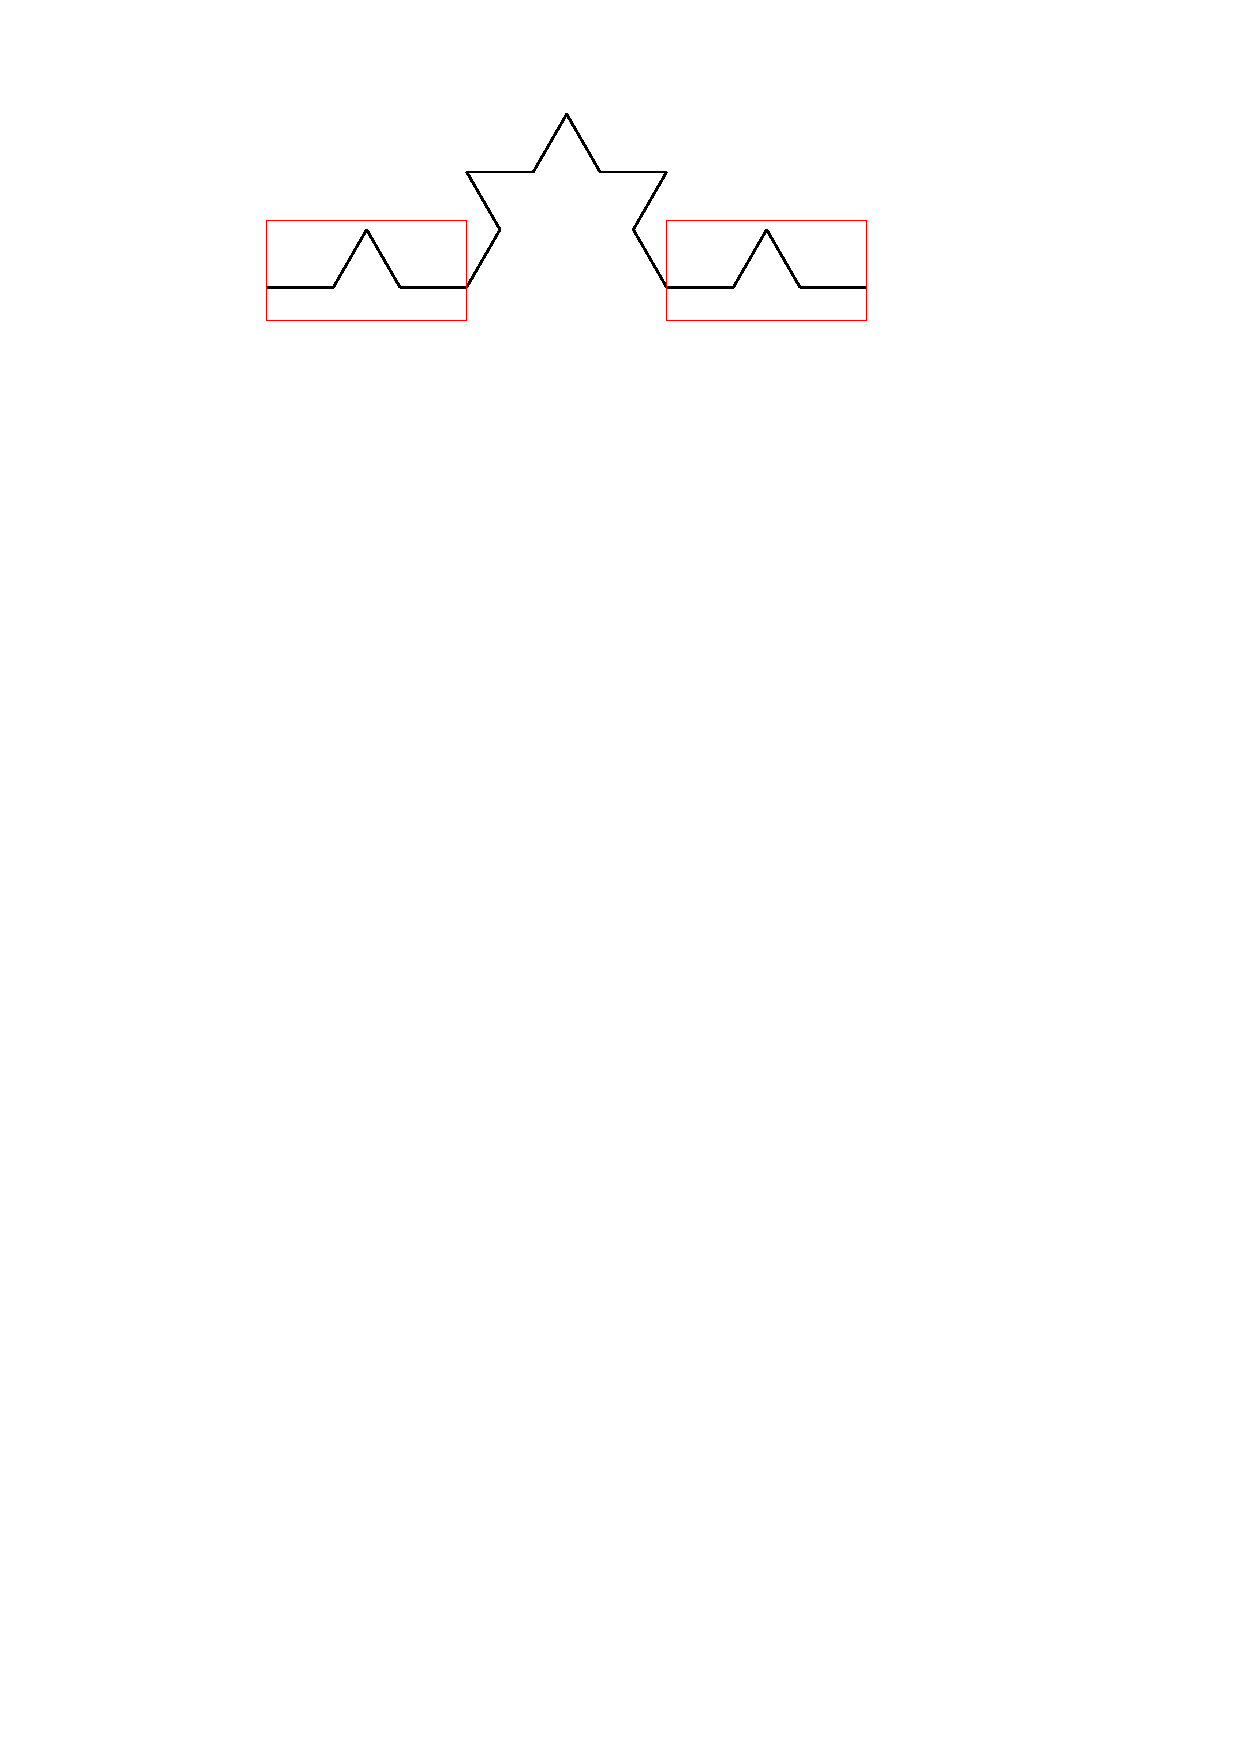
\includegraphics[scale=\normalipe]{ch01-kochova-krivka-podobnost.pdf}
    \caption{První iterace Kochovy křivky "uvnitř" druhé v~menším měřítku.}
    \label{fig:kochova_krivka_podobnost}
\end{figure}
Zkusme se nyní podívat na délku křivky. V~první iteraci začínáme s~úsečkou délky\footnote{Mohli bychom také začít s~obecnou délkou $\ell_0$,~ale ta by se však při výpočtu projevila pouze jako konstantní násobek.} $1$,~která se v~druhé iteraci změní na křivku délky $4/3$. Není těžké si rozmyslet,~že obecně v~$n$-té iteraci bude délka křivky $\ell_n$ rovna
\begin{equation*}
    \left(\dfrac{4}{3}\right)^{n}.
\end{equation*}
Posloupnost $\{\ell_n\}_{n=1}^{\infty}$ je geometrická s~kvocientem $q=4/3>1$,~a tedy její limita je $\infty$. Kochova křivka má tak \emph{nekonečnou délku}.

\subsection{Sierpińského trojúhelník}\label{subsec:sierpinskeho_trojuhelnik}
Přesuneme nyní k~plošným útvarům,~neboť i~zde lze sledovat některé zajímavé vlastnosti. Jedním z~představitelů je tzv. \emph{Sierpińského trojúhelník}\index{Sierpińského trojúhelník}\index{trojúhelník!Sierpińského},~který objevil roku \emph{1916} polský matematik \name{Wacław~Sierpiński} \mbox{(1882--1969)}. \citep[str. 61]{Peitgen2004} Na začátku (v nulté iteraci) začínáme s~rovnostranným trojúhelníkem se stranou délky $1$ (též lze začít s~obecnou délkou $\ell_0$). V~něm sestrojíme střední příčky (tj. spojnice středů stran trojúhelníka),~které společně utvoří strany rovnostranného trojúhelníka\index{trojúhelník!rovnostranný}\index{rovnostranný trojúhelník} čtvrtinového obsahu původního trojúhelníka (to vychází z~faktu,~že střední příčka v~libovolném trojúhelníku má délku rovnou polovině délky strany,~s~níž je rovnoběžná). Obsah nově vzniklého trojúhelníku odebereme a postup opakujeme pro zbývající trojici trojúhelníků v~původním obrazci (viz obrázek \ref{fig:sierpinskeho-trojuhelnik-5iteraci}).\par
\begin{figure}[h]
    \centering
    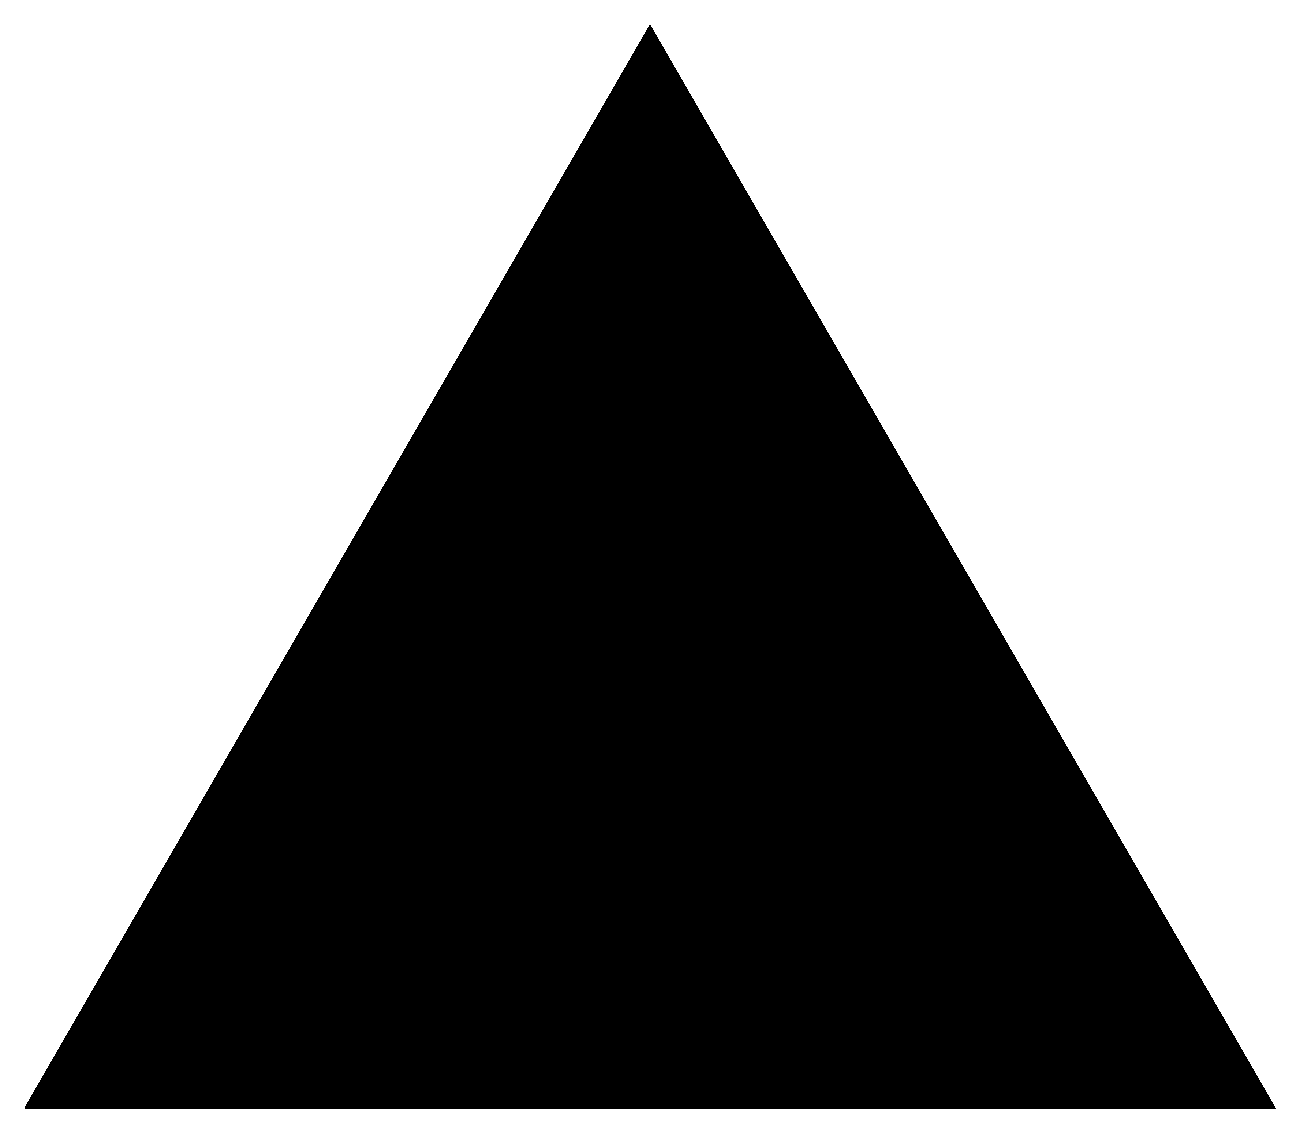
\includegraphics[width=0.4\textwidth]{ch01-sierpinskeho-trojuhelnik-0iterace.pdf}\qquad
    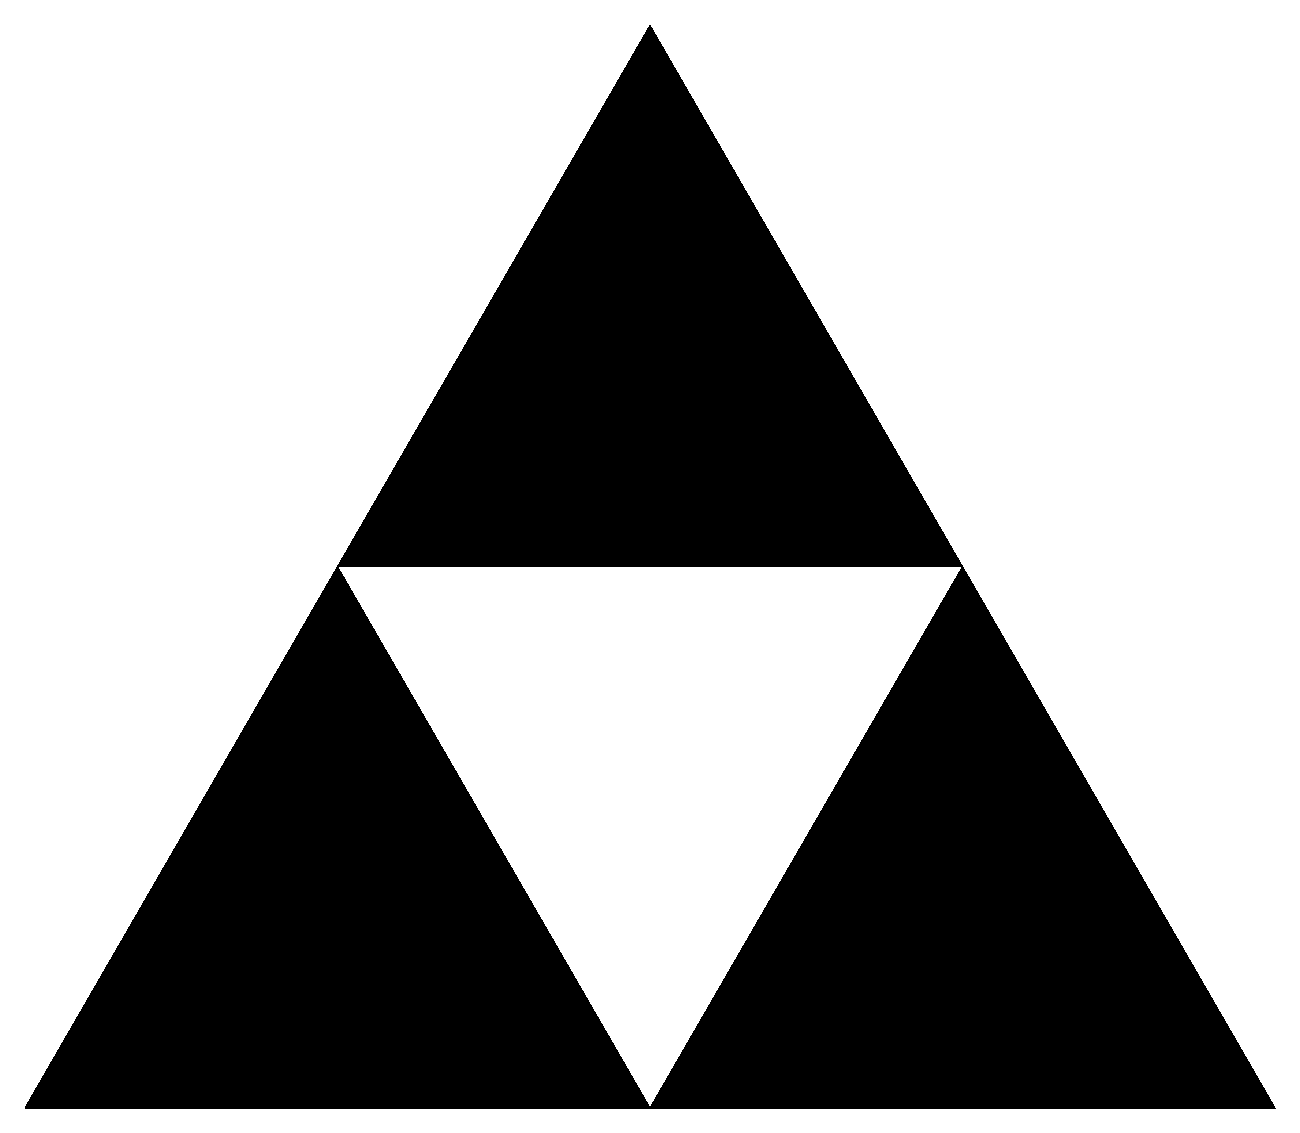
\includegraphics[width=0.4\textwidth]{ch01-sierpinskeho-trojuhelnik-1iterace.pdf}\qquad\\
    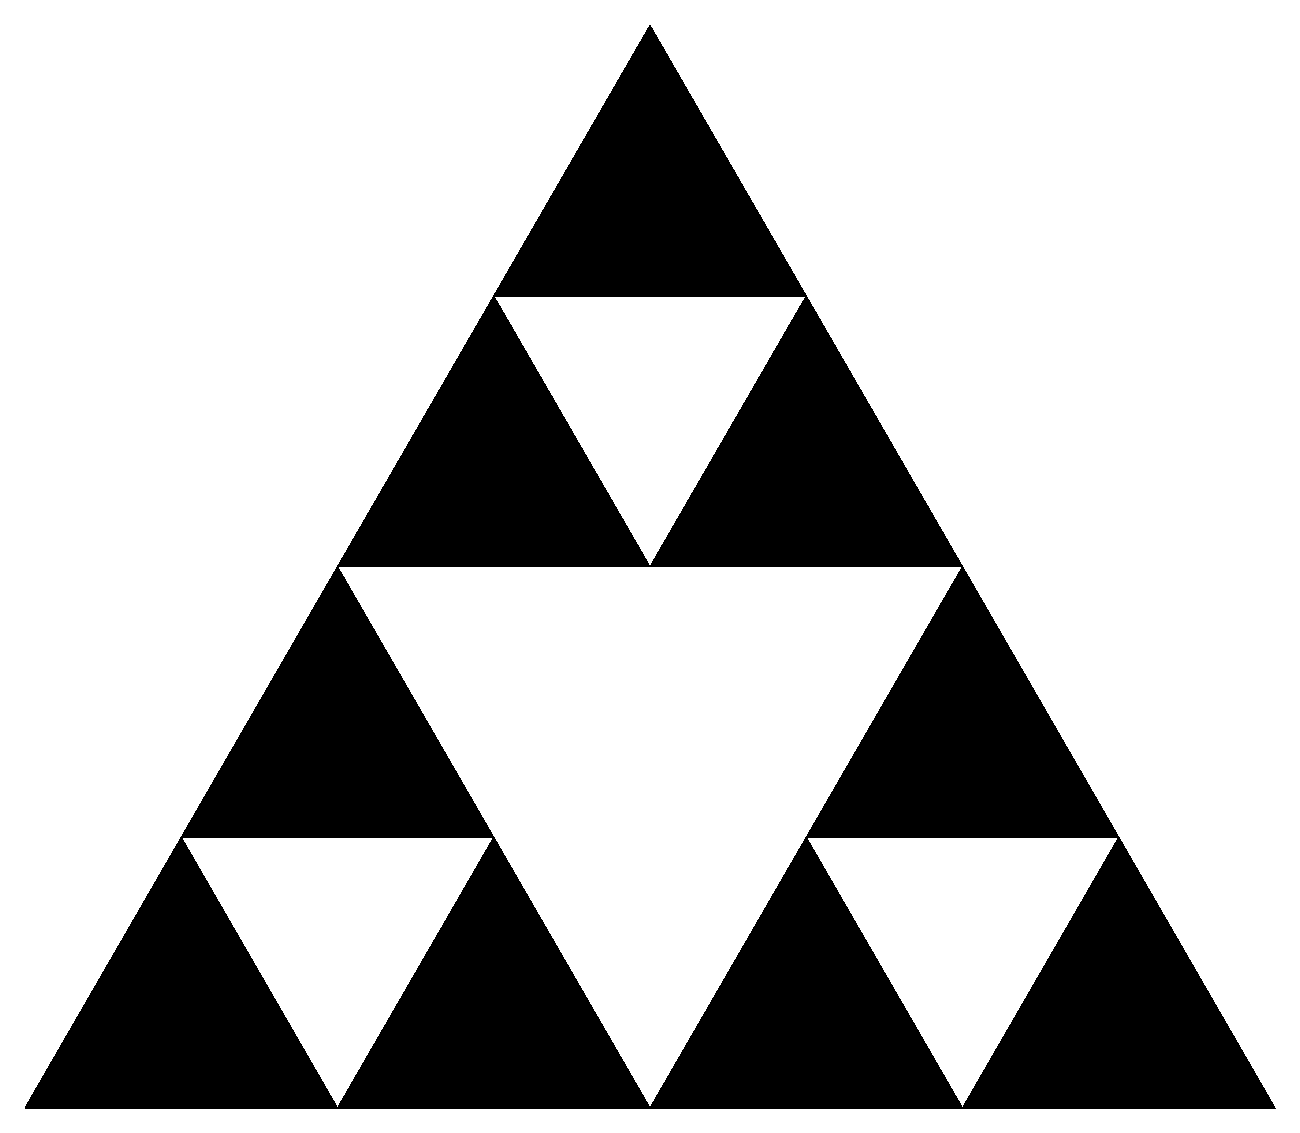
\includegraphics[width=0.4\textwidth]{ch01-sierpinskeho-trojuhelnik-2iterace.pdf}\qquad
    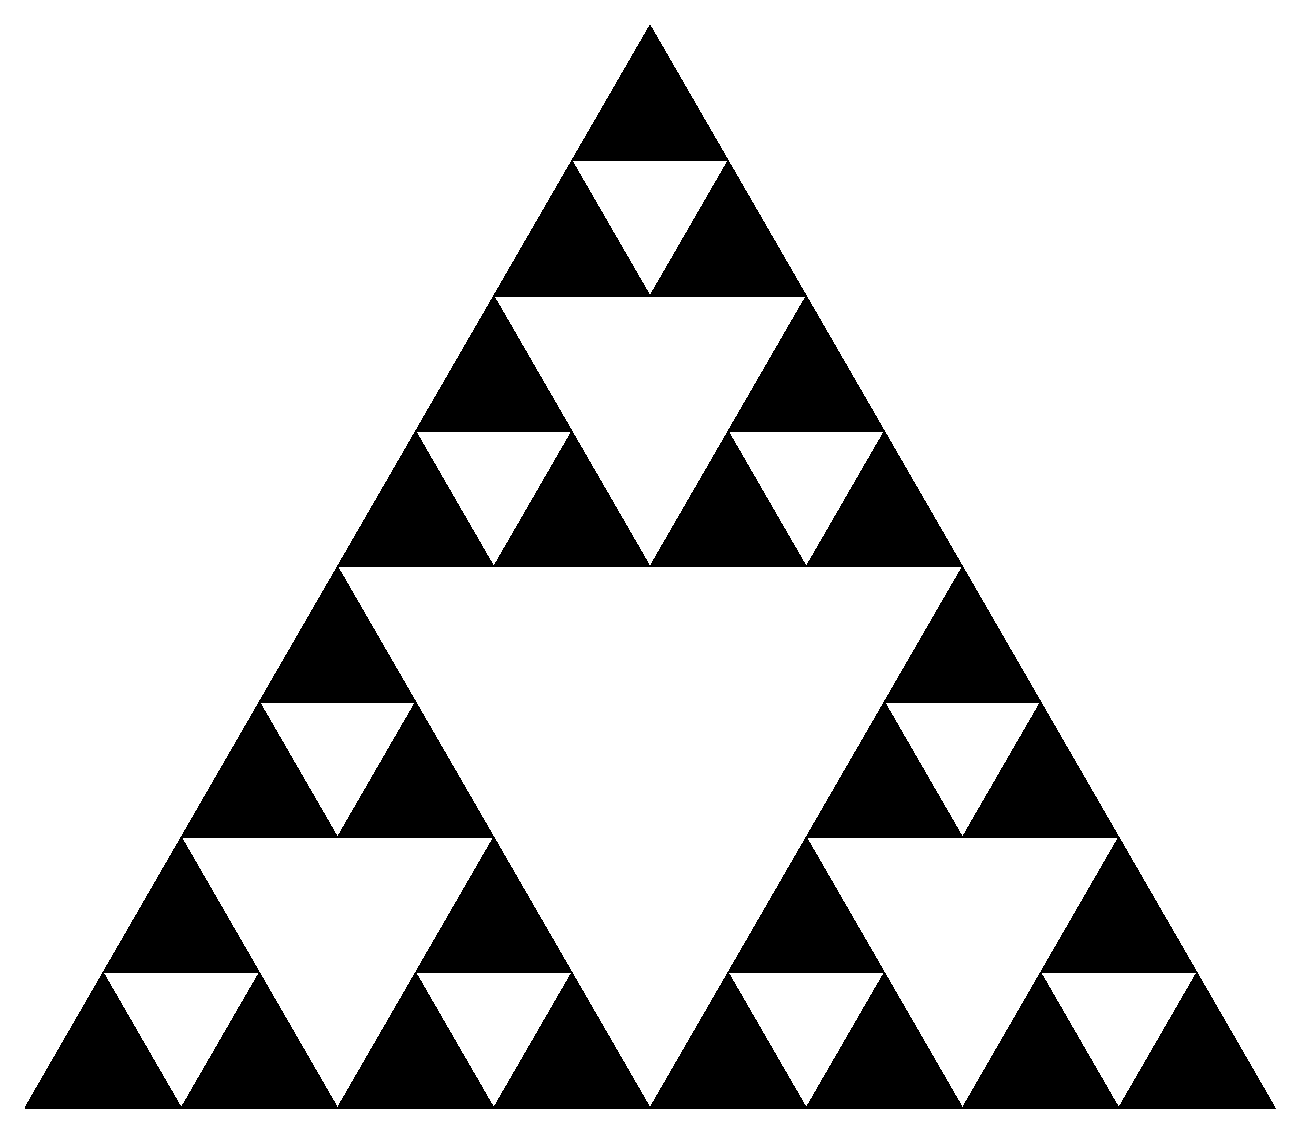
\includegraphics[width=0.4\textwidth]{ch01-sierpinskeho-trojuhelnik-3iterace.pdf}\qquad\\
    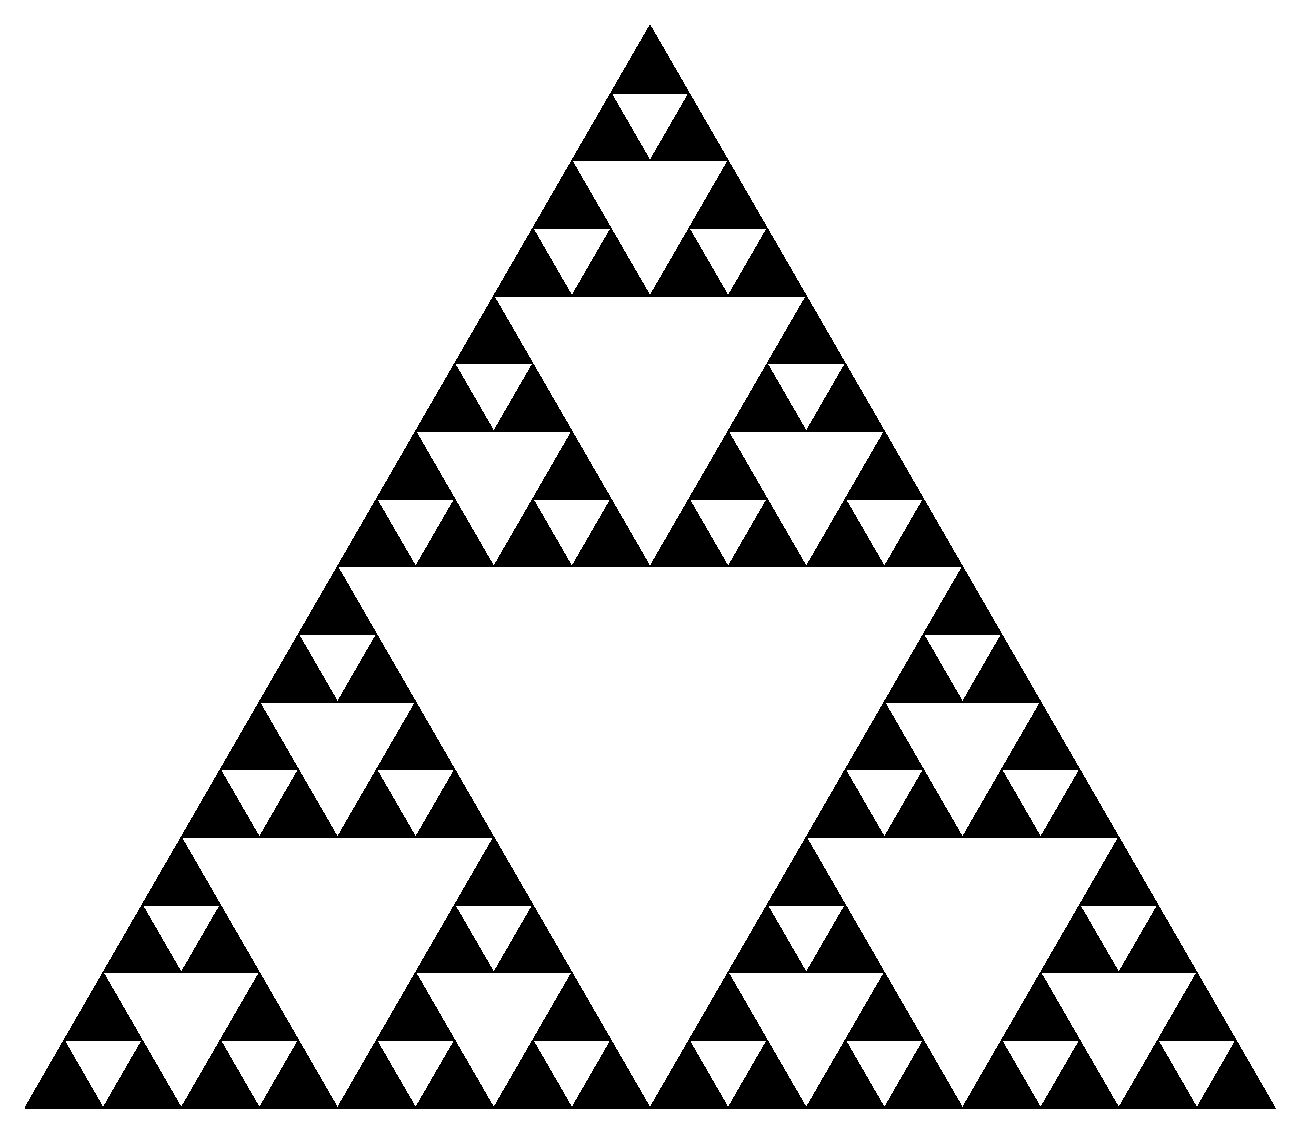
\includegraphics[width=0.4\textwidth]{ch01-sierpinskeho-trojuhelnik-4iterace.pdf}
    \caption{První čtyři iterace Sierpińského trojúhelníka.}
    \label{fig:sierpinskeho-trojuhelnik-5iteraci}
\end{figure}
I zde si lze všimnout,~že po nekonečně mnoha iteracích budou menší trojúhelníky přesnými kopiemi původního obrazce. Zkusme se opět podívat,~jak je to s~obvodem obrazce. Každá ze středních příček,~které vzniknou v~další iteraci,~má poloviční délku vůči délce strany $l$ původního trojúhelníku. Obvod obrazce se tak zvětší o~$3l/2$. Počet trojúhelníků poroste exponenciálně,~neboť v~každé iteraci odstraněním jednoho trojúhelníku vzniknou tři nové,~tj. obvod se po $k$-té iteraci zvětší o~$3^k\cdot(1/2)^k=(3/2)^k$ (na začátku pro $k=0$ je obvod $3$). Obvod obrazce $O_n$ po $n$ iteracích bude roven součtu přírůstků přes všechny iterace,~tj.
\begin{equation}\label{eq:obvod_sierpinskeho_trojuhelniku_niteraci}
    O_n=3+\sum_{k=1}^n{\left(\dfrac{3}{2}\right)^k}.
\end{equation}
Řada $\sum_{k=1}^{n}(3/2)^k$ je geometrická s~kvocientem $3/2$. Zde si vzpomeňme na vzorec pro její součet.
\begin{theorem}[Součet geomerické řady]\label{thm:soucet_geometricke_rady}
    Nechť je dána geometrická posloupnost $\{g_k\}_{k=1}^\infty$ s~kvocientem $q\neq 1$. Pak pro součet prvních $n$ členů platí
    \begin{equation*}
        \sum_{k=1}^{n}{g_k}=g_1\dfrac{1-q^n}{1-q}.
    \end{equation*}
\end{theorem}
\begin{proof}
    Důkaz vzorce zde vynecháme,~nicméně čtenář si jej může snadno ověřit např. indukcí podle $n$. 
\end{proof}
Celkově tak po aplikaci vzorce z~\ref{thm:soucet_geometricke_rady} v~rovnosti \eqref{eq:obvod_sierpinskeho_trojuhelniku_niteraci} dostaneme po jednoduché úpravě
\begin{equation*}
    O_n=3+\sum_{k=1}^n{\left(\dfrac{3}{2}\right)^k}=3+\dfrac{3}{2}\cdot\dfrac{\left(\dfrac{3}{2}\right)^n-1}{\dfrac{3}{2}-1}=3+3\left(\left(\dfrac{3}{2}\right)^n-1\right)=3\left(\dfrac{3}{2}\right)^n.
\end{equation*}
Posloupnost $\{O_n\}_{n=0}^\infty$ je opět geometrická s~kvocientem $q=3/2>1$,~tzn. její limita je opět $\infty$. Obvod Sierpińského trojúhelníku\index{Sierpińského trojúhelník}\index{trojúhelník!Sierpińského} tedy roste nade všechny meze. (Výpočet jsme si mohli též zjednodušit uvědoměním si,~že obvod obrazce roste s~faktorem $3/2$ a vzorec pro $O_n$ jsme tak mohli určit ihned.)\par
Podívejme se nyní na obsah útvaru. Zde si již výpočet trochu usnadníme. Po každé iteraci se jeho obsah zmenší na $3/4$ obsahu původního obrazce. Lze snadno odvodit,~že obsah rovnostranného trojúhelníku o~straně délky $a$ je
\begin{equation*}
    \dfrac{\sqrt{3}}{4}a^2
\end{equation*}
Na začátku je obsah útvaru $S_0=\sqrt{3}/4$. Tj. celkově po $n$-iteracích bude obsah $S_n$ roven
\begin{equation}\label{eq:obsah_sierpinskeho_trojuhelniku}
    \dfrac{\sqrt{3}}{4}\left(\dfrac{3}{4}\right)^n
\end{equation}
Výraz \eqref{eq:obsah_sierpinskeho_trojuhelniku} má pro $n\to\infty$ limitu nulovou,~tedy zatímco Sierpińského trojúhelník má \emph{nekonečný obvod},~jeho obsah je však naopak \emph{nulový}.

\subsection{Kochova vločka}\label{subsec:kochova_vlocka}
Rozšiřující variantou Kochovy křivky \ref{subsec:kochova_krivka} je tzv. \emph{Kochova vločka}\index{Kochova vločka}\index{vločka!Kochova},~která se skládá ze tří Kochových křivek\index{Kochova křivka}\index{křivka!Kochova}. Rozdíl je zde v~tom,~že začínáme s~rovnostranným trojúhelníkem o~straně délky $1$. Na každou ze stran aplikujeme stejný proces,~jako předtím,~tj. odebereme prostřední třetinu,~nahradíme ji dvěma na sebe navazujícími úsečkami délek $1/3$ a opakujeme pro každou nově vzniklou úsečku (viz obrázky \ref{fig:kochova_vlocka_dve_iterace} a \ref{fig:kochova_krivka_5iterace}).
\begin{figure}[h]
    \centering
    \begin{subfigure}{\subfigwidth}
        \centering
        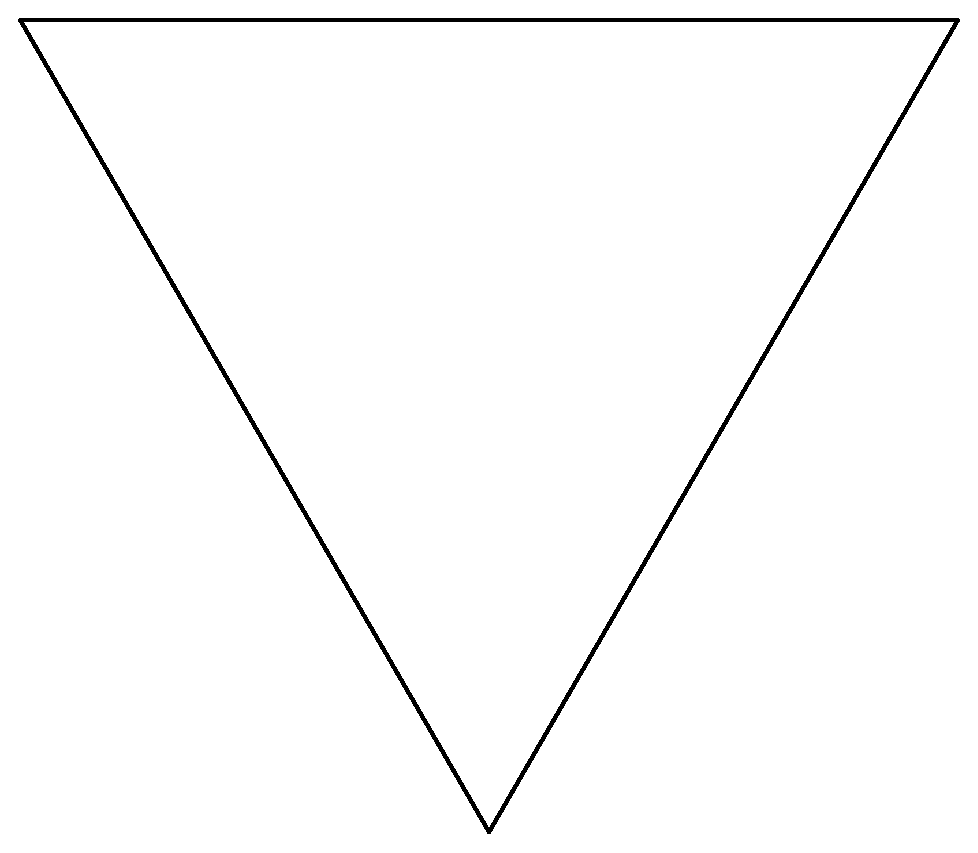
\includegraphics[scale=\fractalscale]{ch01-kochova-vlocka-0iterace.pdf}
    \end{subfigure}
    \qquad
    \begin{subfigure}{\subfigwidth}
        \centering
        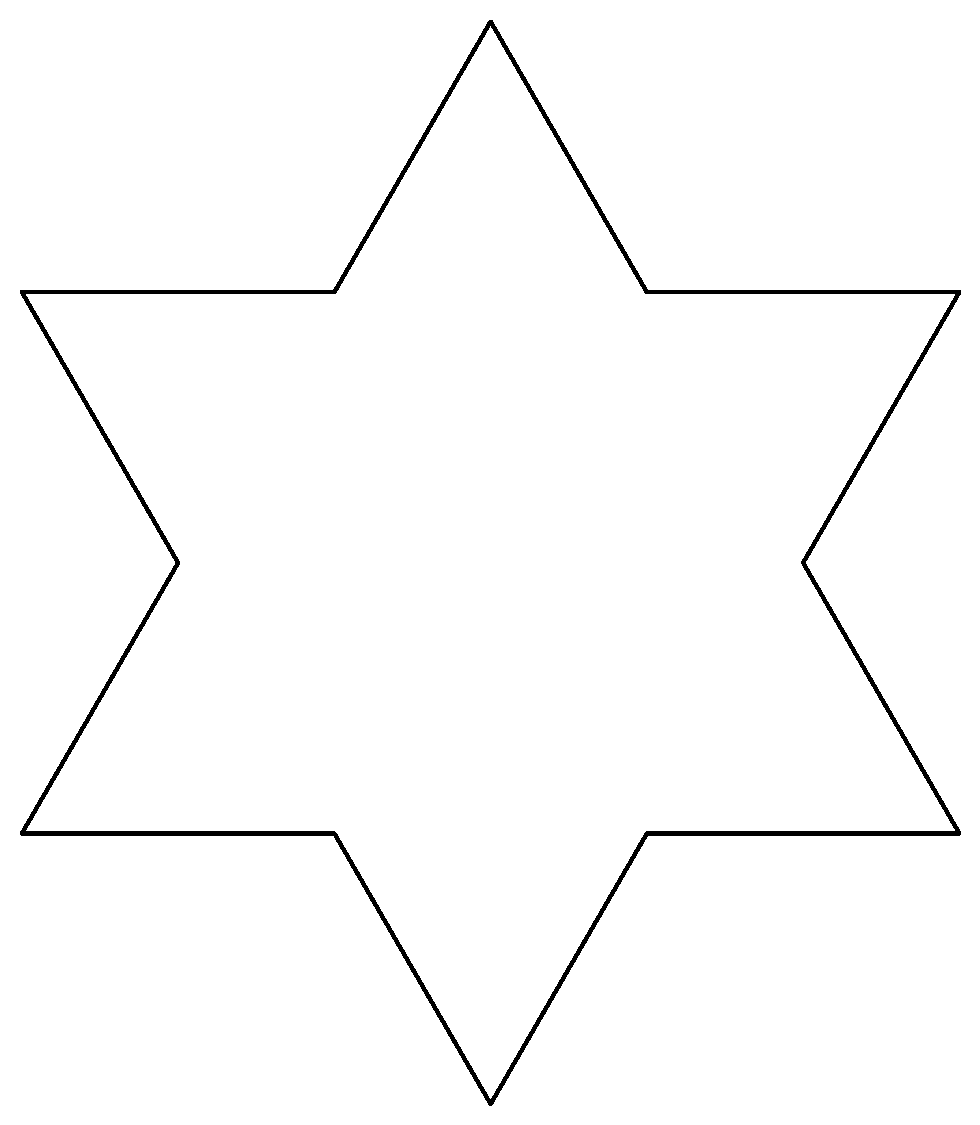
\includegraphics[scale=\fractalscale]{ch01-kochova-vlocka-1iterace.pdf}
    \end{subfigure}
    \caption{Nultá a první iterace Kochovy vločky.}
    \label{fig:kochova_vlocka_dve_iterace}
\end{figure}
\begin{figure}[h]
    \centering
    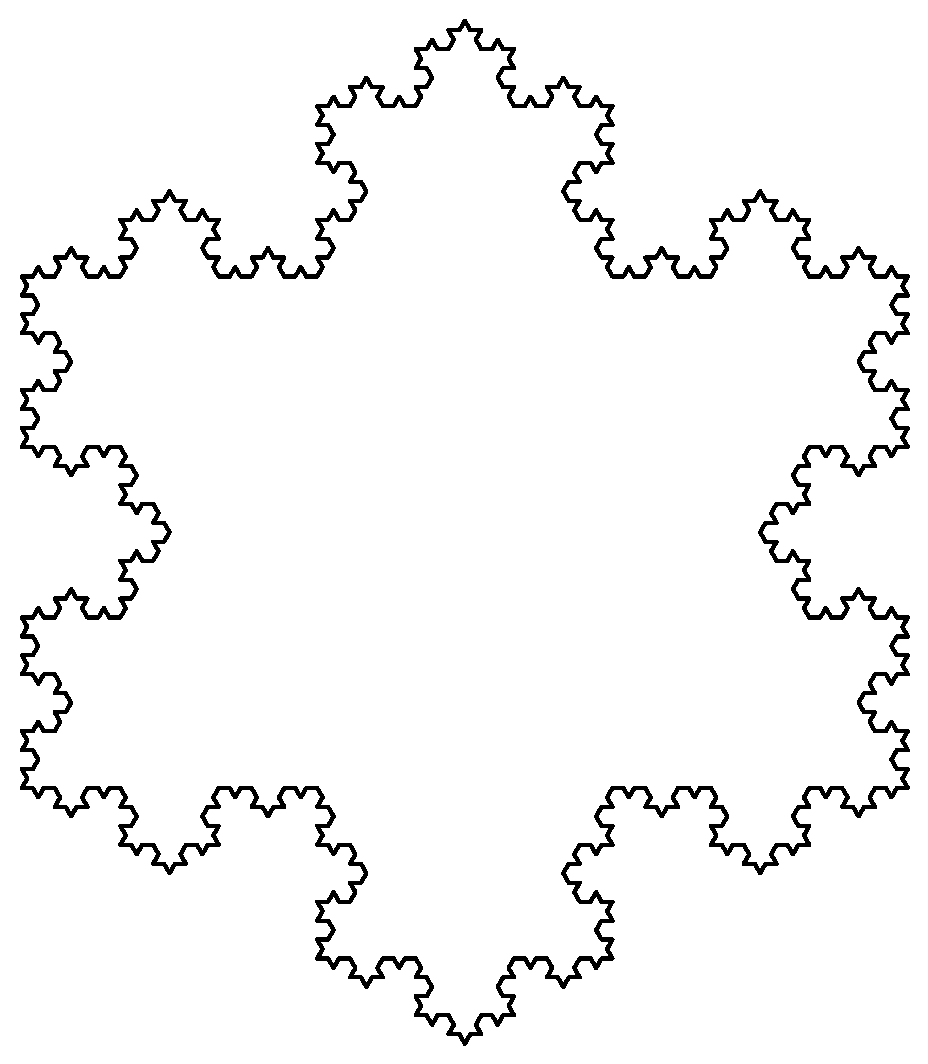
\includegraphics[scale=\fractalscale]{ch01-kochova-vlocka-4iterace.pdf}
    \caption{Čtvrtá iterace Kochovy vločky.}
    \label{fig:kochova_krivka_5iterace}
\end{figure}
Podíváme-li se na obvod,~nejspíše nás nepřekvapí,~že ten je i~zde nekonečný\footnote{Obvod Kochovy křivky po $n$-té iteraci je $o_n=3\cdot(4/3)^{n}$.} (už z~principu,~že každá strana původního rovnostranného trojúhelníka představuje samostatnou Kochovu křivku).
Obsah vzniklého útvaru je však již zajímavější. Pro zjednodušení výpočtu si rozdělme útvar na \emph{stejné rovnostranné trojúhelníky} podle obrázku \ref{fig:kochova_vlocka_rozdeleni},~jejichž obsah je roven $1/12$ obsahu obrazce v~nulté iteraci.
\begin{figure}[h]
    \centering
    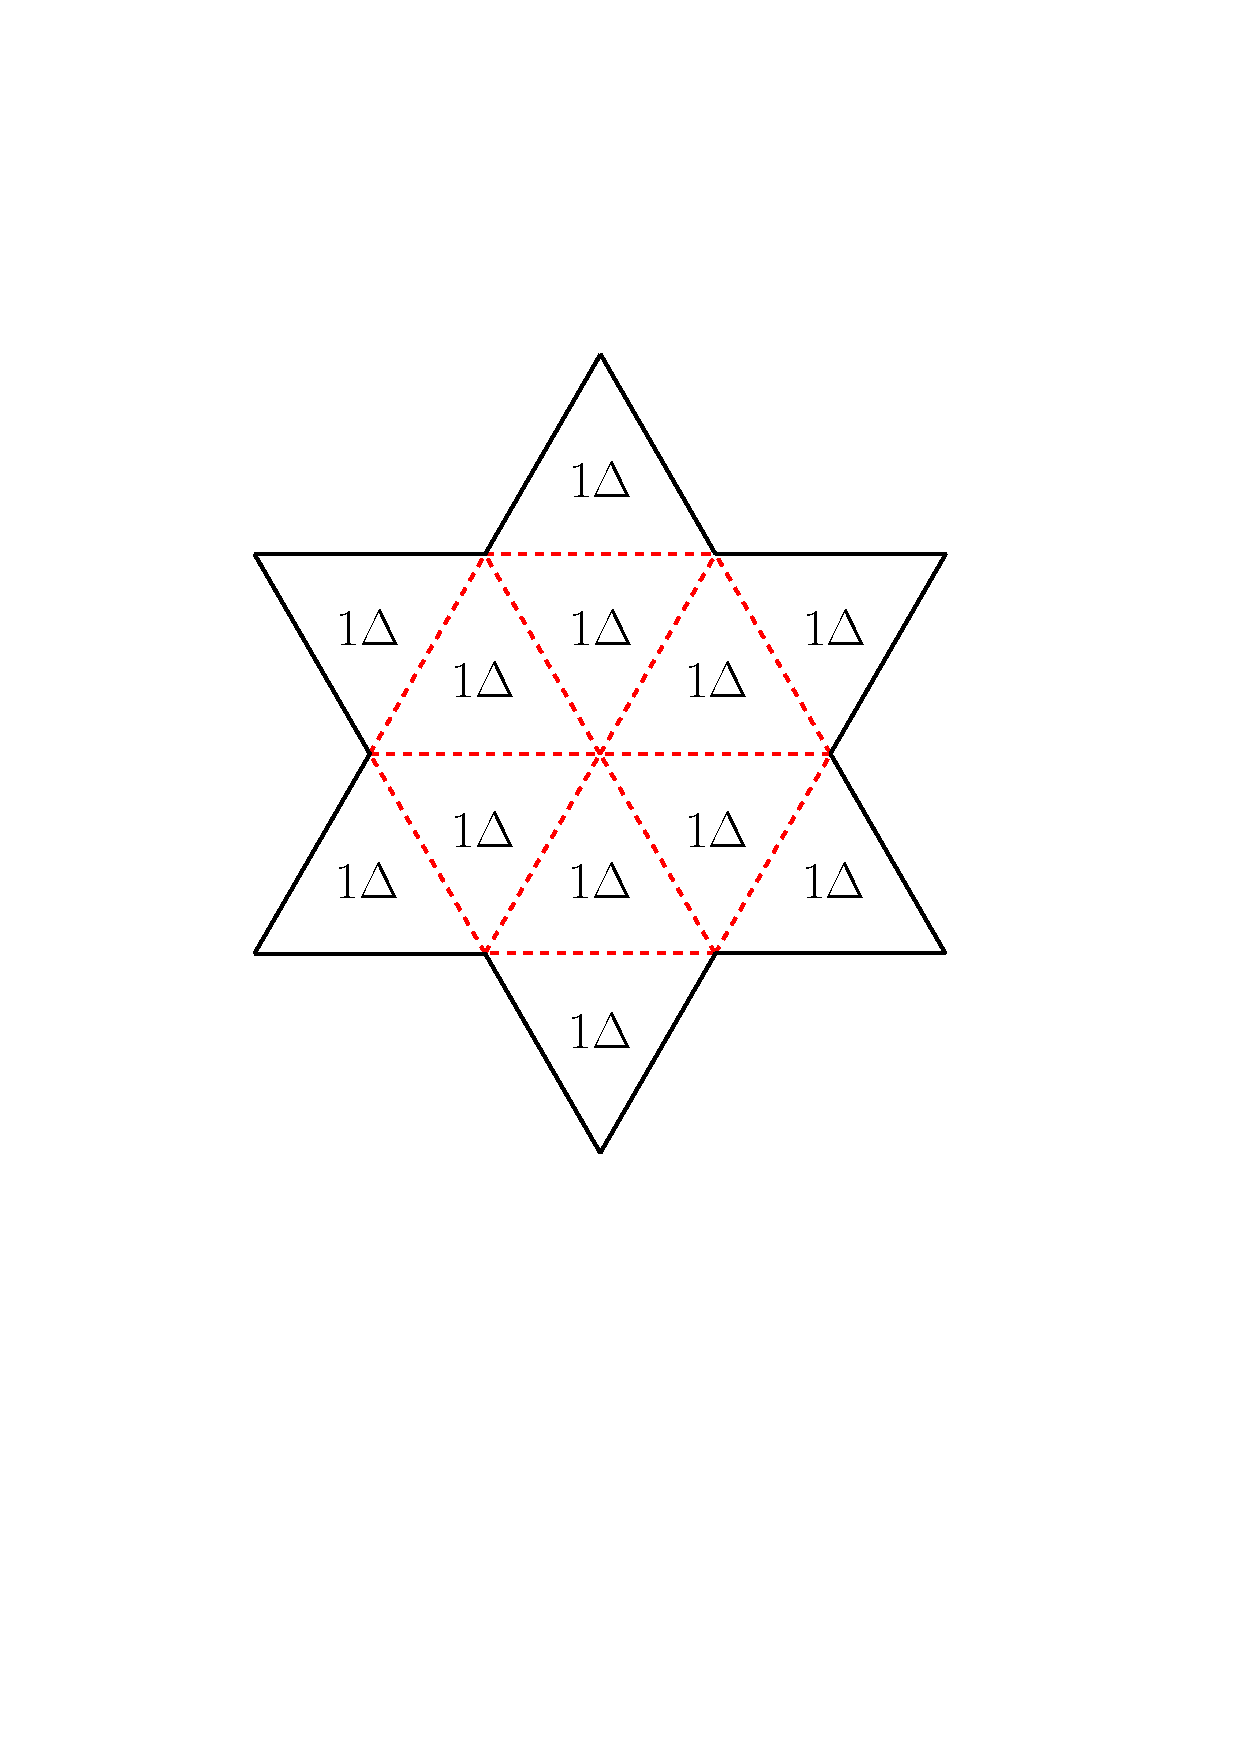
\includegraphics[scale=.4]{ch01-kochova-vlocka-rozdeleni.pdf}
    \caption{Rozdělení první iterace Kochovy vločky.}
    \label{fig:kochova_vlocka_rozdeleni}
\end{figure}
Výsledný obsah se tedy pokusíme vyjádřit relativně vůči \emph{obsahům daných trojúhelníků},~na něž jsme obrazec rozdělili,~a pak jej pouze přepočítáme. Jejich obsah si označme $\Delta$. Tedy obsah Sierpińského trojúhelníku v~nulté iteraci lze vyjádřit jako $S_0=9\Delta$. Po první iteraci vzniknou na každé ze strany 3 nové trojúhelníky o~obsahu $1/9\cdot\Delta$. V~každé další iteraci vzniknou z~jedné úsečky 4 nové. Obecně po $n$ iteracích jich tedy bude $3\cdot 4^{n}$. (Při výpočtu musíme počítat s~o jedna nižší mocninou,~neboť trojúhelníky vznikají "na úsečkách" z~předešlé iterace,~nikoliv té aktuální.)\par
Zaměřme se nyní pouze trojúhelníky,~které vznikly v~aktuální iteraci (viz obrázek \ref{fig:kochova_vlocka_2iterace_nove_trojuhelniky}). Součet jejich obsahů nám dává \emph{přírůstek obsahu} v~obecné $n$-té iteraci. Označíme-li tento přírůstek $B_n$,~pak platí
\[B_n=\underbrace{3\cdot 4^{n-1}}_{\text{počet úseček}}\cdot\overbrace{\left(\dfrac{1}{9}\right)^{n-1}\Delta}^{\text{obsah nových troj.}}=3\cdot\left(\dfrac{4}{9}\right)^{n-1}\Delta,\]
kde $n\geqslant 1$.
\begin{figure}[h]
    \centering
    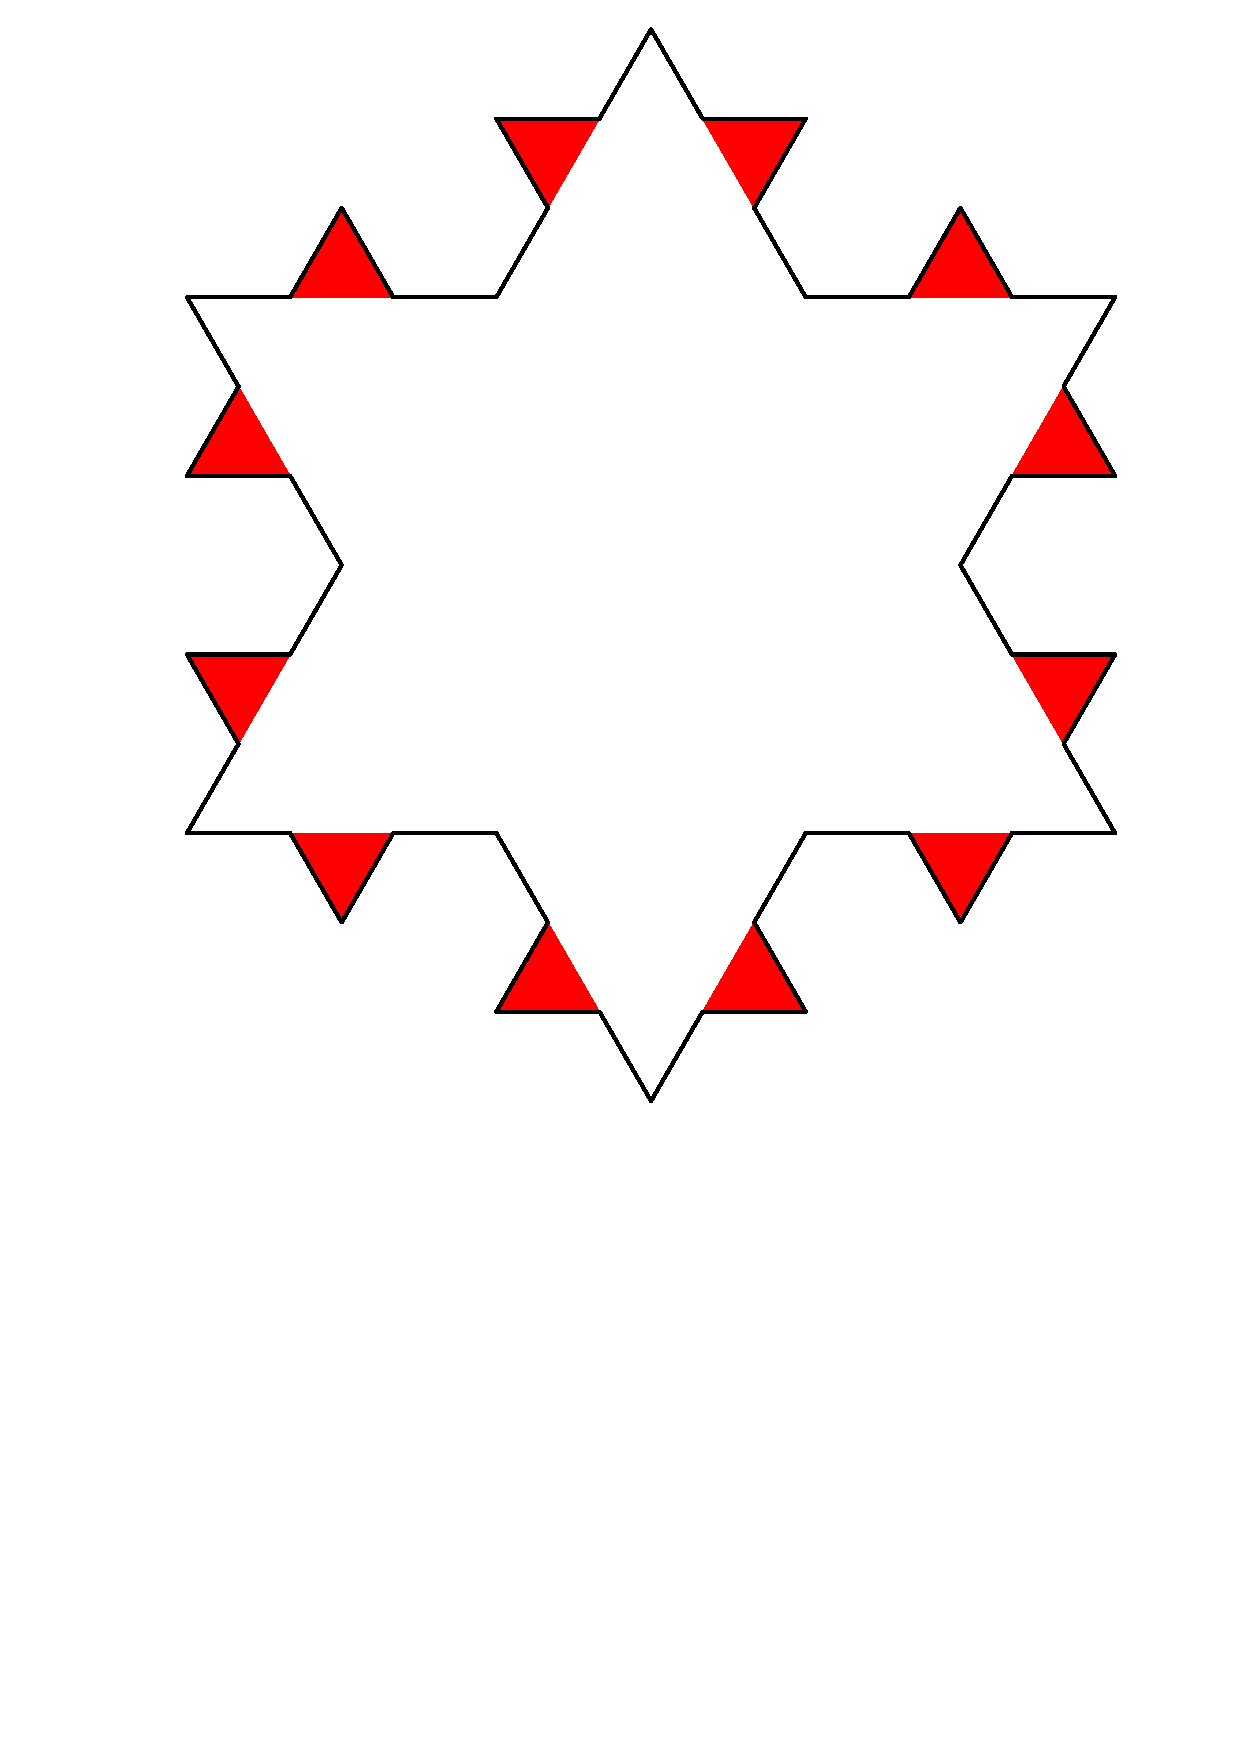
\includegraphics[scale=\fractalscale]{ch01-kochova-vlocka-2iterace-nove-trojuhelniky.pdf}
    \caption{Nově vzniklé trojúhelníky v~druhé iteraci.}
    \label{fig:kochova_vlocka_2iterace_nove_trojuhelniky}
\end{figure}
Nyní můžeme již vyšetřit obsah v~$n$-té iteraci $S_n$ a posléze i~celkový obsah výsledného obrazce $S=\lim_{n\to\infty}{S_n}$. Pro $n\geqslant 1$ platí
\begin{align*}
    S_n&=S_0+\sum_{k=1}^{n}{B_k}=9\Delta+3\Delta\cdot\sum_{k=1}^{n}{\left(\dfrac{4}{9}\right)^{k-1}}=9\Delta+3\Delta\cdot\dfrac{1-\left(\dfrac{4}{9}\right)^{n}}{1-\dfrac{4}{9}}\\
    &=9\Delta+\dfrac{27}{5}\Delta\cdot\left(1-\left(\dfrac{4}{9}\right)^n\right)
\end{align*}
Tedy
\begin{align*}
    S&=\lim_{n\to\infty}{S_n}=9\Delta+\dfrac{27}{5}\Delta\cdot\left(1-\left(\dfrac{4}{9}\right)^n\right)=9\Delta+\dfrac{27}{5}\Delta\cdot\left(1-\lim_{n\to\infty}\left(\dfrac{4}{9}\right)^n\right)\\
    &=9\Delta+\dfrac{27}{5}\Delta=\dfrac{72}{5}\Delta.
\end{align*}
Obsah trojúhelníků,~na než jsme rozdělili první iteraci Kochovy vločky,~je
\[\Delta=\dfrac{\sqrt{3}}{4}\cdot\dfrac{1}{9}\]
a tedy celkově
\[S=\dfrac{72}{5}\Delta=\dfrac{72}{5}\cdot\dfrac{\sqrt{3}}{4}\cdot\dfrac{1}{9}=\dfrac{2\sqrt{3}}{5}.\]
Byl to trochu delší výpočet,~nicméně jsme zjistili,~že Kochova vločka má (stejně jako Kochova křivka) \emph{nekonečnou délku (obvod)},~ale obsah má \emph{konečný}.
% Obsah vzniklého útvaru je však již zajímavější. Po první iteraci přibudou 3 nové trojúhelníky se stranou délky $1/3$,~tzn. jejich obsah bude
% \begin{equation*}
%     \dfrac{\sqrt{3}}{4}\left(\dfrac{1}{3}\right)^2
% \end{equation*}
% a celkový obsah obrazce tedy bude
% \begin{equation*}
%     S_1=\dfrac{\sqrt{3}}{4}+3\cdot\dfrac{\sqrt{3}}{4}\left(\dfrac{1}{3}\right)^2.
% \end{equation*}
% V~každé další iteraci vzniknou z~jedné úsečky 4 nové. Obecně po $n$ iteracích jich bude $3\cdot 4^n$ (při výpočtu však musíme počítat s~o jedna nižší mocninou,~neboť trojúhelníky vznikají "na úsečkách" z~předešlé iterace,~nikoliv té aktuální,~viz obrázek \ref{fig:kochova_vlocka_2iterace_nove_trojuhelniky}).
% \begin{figure}[h]
%     \centering
%     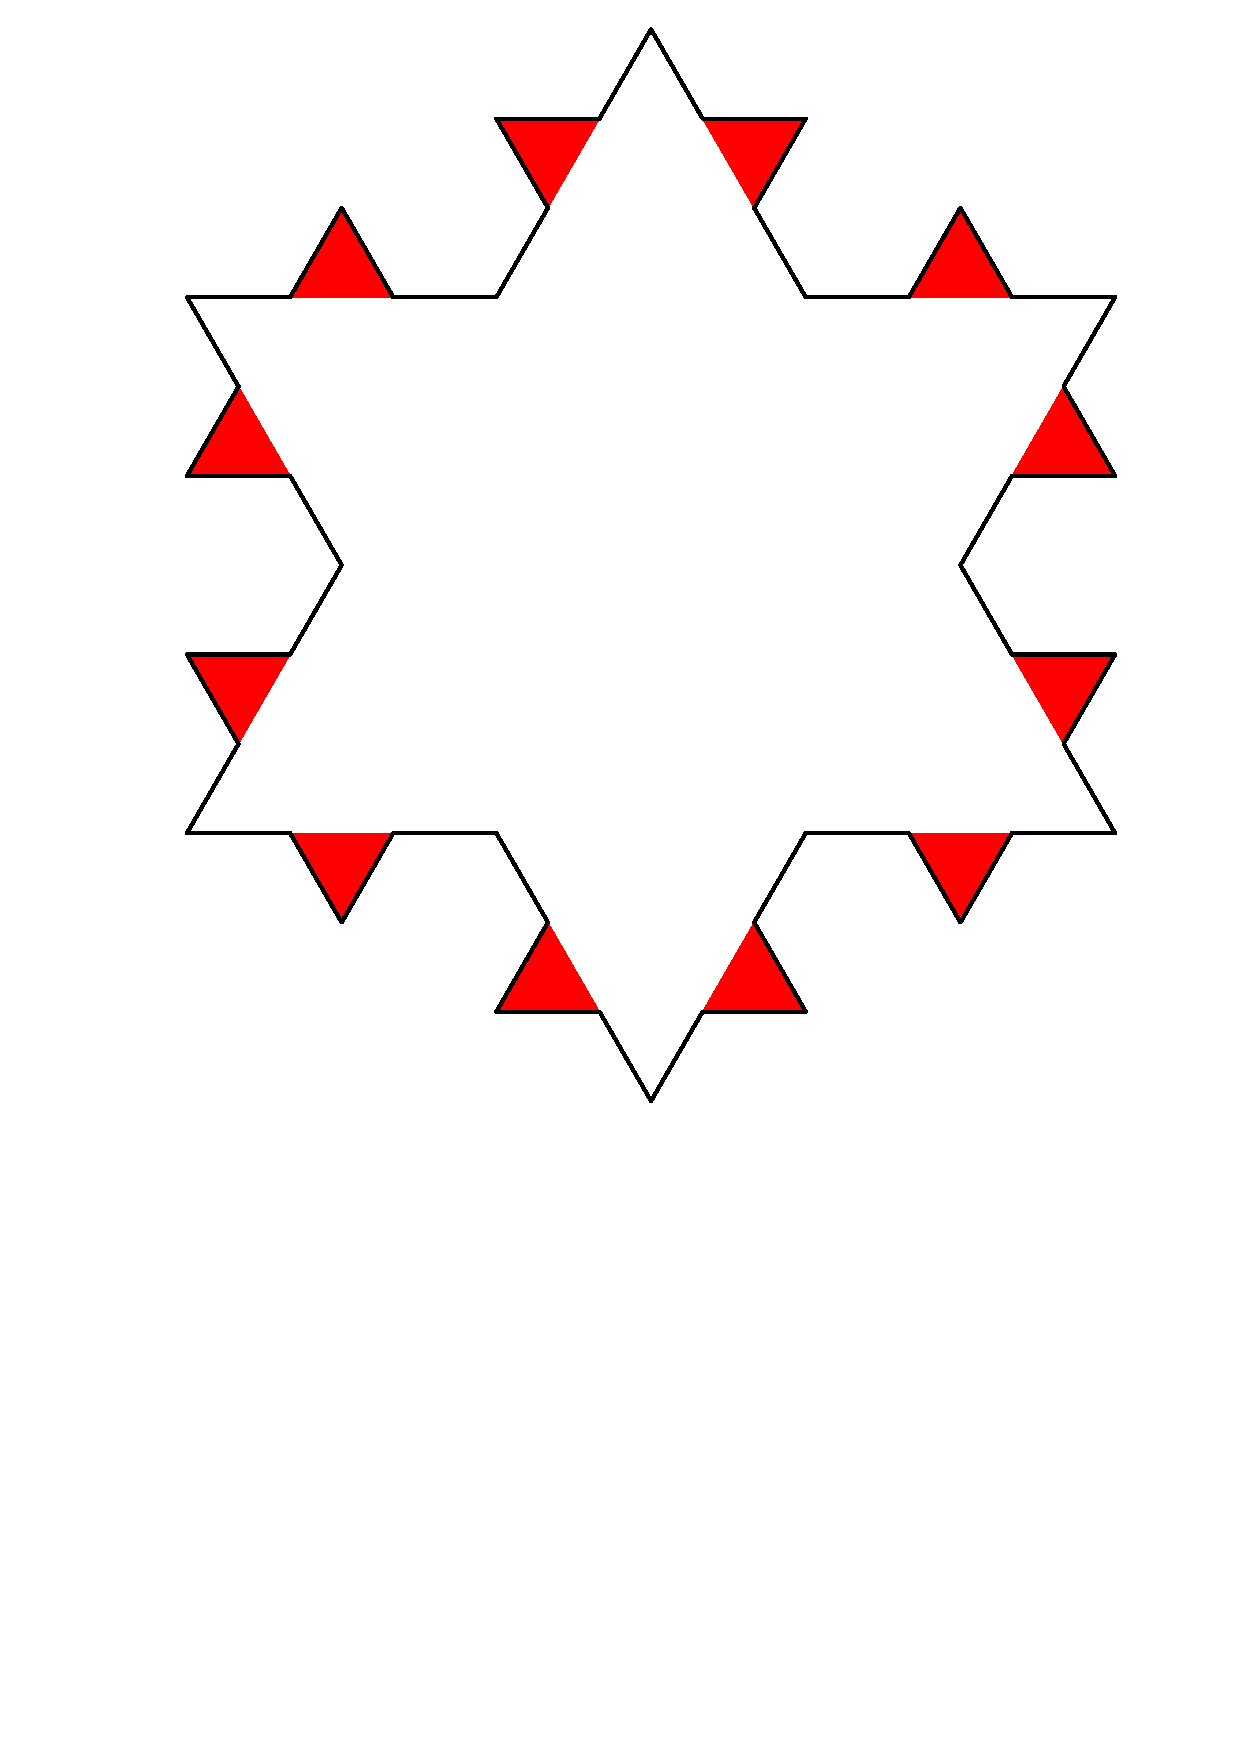
\includegraphics[scale=\fractalscale]{ch01-kochova-vlocka-2iterace-nove-trojuhelniky.pdf}
%     \caption{Nově vzniklé trojúhelníky v~druhé iteraci.}
%     \label{fig:kochova_vlocka_2iterace_nove_trojuhelniky}
% \end{figure}
% Délka úseček,~a tedy i~stran nově vzniklých rovnostranných trojúhelníků,~je $(1/3)^n$. Celkový obsah nově vzniklých trojúhelníků je tak
% \begin{equation}\label{eq:obsah_novych_trojuhelniku}
%     3\cdot 4^{n-1}\cdot\dfrac{\sqrt{3}}{4}\left(\dfrac{1}{3^n}\right)^2.
% \end{equation}
% Pro další výpočet bude pro nás výhodné si výraz \eqref{eq:obsah_novych_trojuhelniku} upravit.
% \begin{equation*}
%     3\cdot 4^{n-1}\cdot\dfrac{\sqrt{3}}{4}\left(\dfrac{1}{3^n}\right)^2=\dfrac{3\sqrt{3}}{4^2}\cdot \dfrac{4^n}{3^{2n}}=\dfrac{3\sqrt{3}}{16}\left(\dfrac{4}{9}\right)^n.
% \end{equation*}
% Celkový obsah obrazce po $n$ iteracích lze tak vypočítat součtem obsahů všech vzniklých trojúhelníků ve všech předešlých iteracích,~tj.
% \begin{equation*}
%     S_n=\sum_{k=1}^n{S_k}=\overbrace{\dfrac{\sqrt{3}}{4}}^{S_0}+\sum_{k=1}^n{\dfrac{3\sqrt{3}}{16}\left(\dfrac{4}{9}\right)^k}.
% \end{equation*}
% Suma na pravé straně představuje geometrickou řadu s~kvocientem $4/9$. Úpravou získáme
% \begin{equation}\label{eq:kochova_vlocka_obsah_n_iteraci}
%     \dfrac{\sqrt{3}}{4}+\dfrac{3\sqrt{3}}{16}\sum_{k=1}^n{\left(\dfrac{4}{9}\right)^k}=\dfrac{\sqrt{3}}{4}+\dfrac{3\sqrt{3}}{16}\cdot\dfrac{4}{9}\cdot\dfrac{1-\left(\dfrac{4}{9}\right)^n}{1-\dfrac{4}{9}}=\dfrac{\sqrt{3}}{4}+\dfrac{3\sqrt{3}}{20}\left(1-\left(\dfrac{4}{9}\right)^n\right)
% \end{equation}
% Můžeme si všimnout,~že výraz \eqref{eq:kochova_vlocka_obsah_n_iteraci} bude tentokrát již konečné číslo,~neboť limitním přechodem pro $n\to\infty$ se výraz $(4/9)^n$ bude blížit nule. Celkově tedy máme
% \begin{align*}
%     S&=\lim_{n\to\infty}S_n=\lim_{n\to\infty}\left(\dfrac{\sqrt{3}}{4}+\dfrac{3\sqrt{3}}{20}\left(1-\left(\dfrac{4}{9}\right)^n\right)\right)=\dfrac{\sqrt{3}}{4}+\dfrac{3\sqrt{3}}{20}\left(1-\lim_{n\to\infty}\left(\dfrac{4}{9}\right)^n\right)\\
%     &=\dfrac{\sqrt{3}}{4}+\dfrac{3\sqrt{3}}{20}=\dfrac{2\sqrt{3}}{5}.
% \end{align*}

\subsection{Cantorovo diskontinuum}\label{subsec:cantorovo_diskontinuum}
Podívejme se ještě na jeden typ fraktálního objektu,~kterým je tzv. \emph{Cantorovo diskontinuum}\footnote{Též se mu říká \emph{Cantorova množina} (angl. \emph{"Cantor set"})\index{Cantorovo diskontinuum}\index{diskontinuum!Cantorovo}. Dvourozměrnou variantou je pak tzv. \emph{Cantorův prach}\index{Cantorův prach}\index{prach!Cantorův} (angl. \emph{"Cantor dust"}). Slovo \emph{prach} je zde míněno v~přeneseném významu,~neboť (podobně jako v~této podsekci) lze ukázat,~že vzniklé útvary mají v~limitě nulový obsah.} Myšlenka je zde velmi jednoduchá: začínáme s~úsečkou délky $1$ (nultá iterace) a následně odebereme prostřední třetinu,~čímž vznikne první iterace. V~dalších iteracích postupujeme analogicky pro vzniklé úsečky (viz obrázek \ref{fig:cantorovo_diskontinuum}).
\begin{figure}[h]
    \centering
    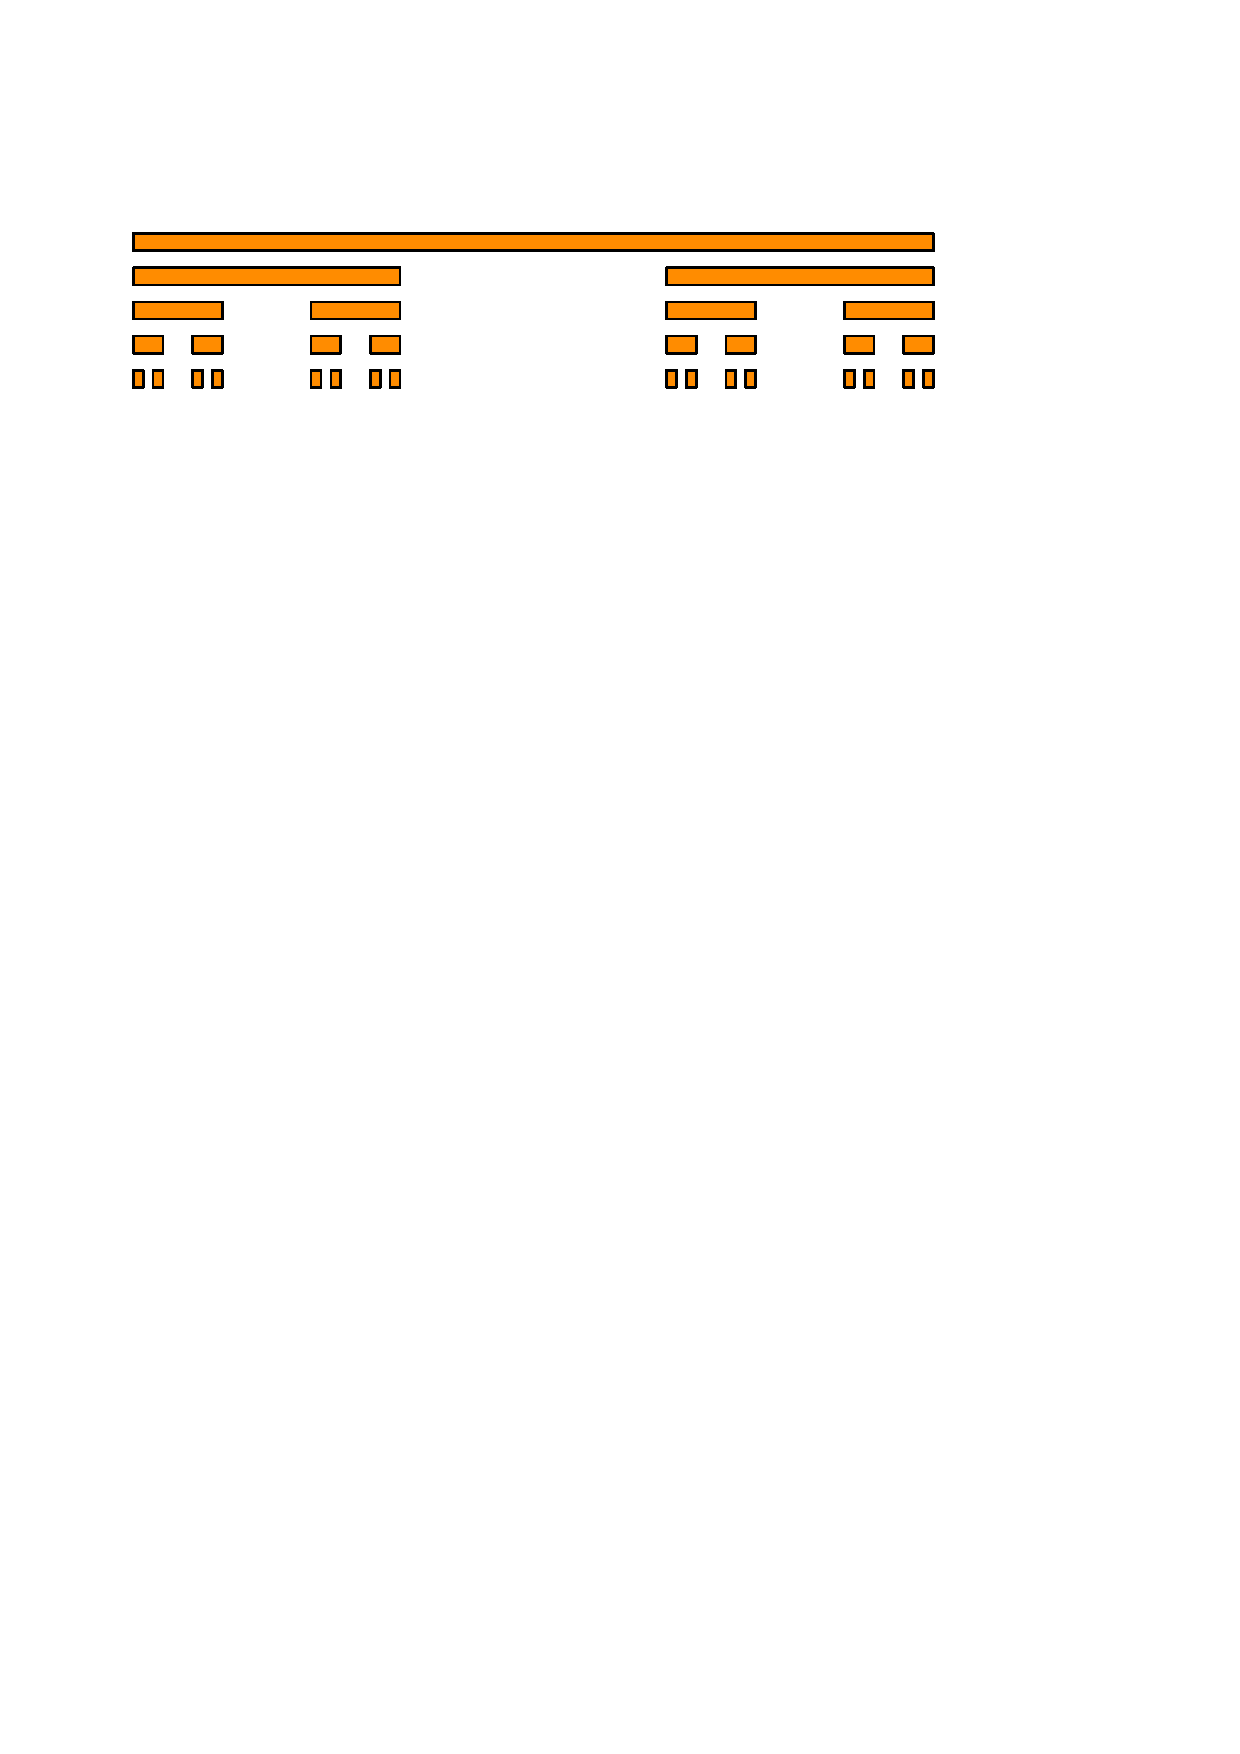
\includegraphics[scale=\normalipe]{ch01-cantorova-mnozina.pdf}
    \caption{Nultá až čtvrtá iterace Cantorova diskontinua.}
    \label{fig:cantorovo_diskontinuum}
\end{figure}

Nově vzniklé úsečky třetinové délky jsou kopiemi původní úsečky. Stejně jako u~předešlých fraktálů nás i~zde bude zajímat limitní chování tohoto procesu. Lze očekávat,~že postupným odebíráním zbudou úsečky nulové délky. O~tom se lze přesvědčit např. tak,~že spočítáme limitu celkových délek všech odebraných úseků. V~první iteraci odebereme úsečku délky $1/3$,~v~druhé iteraci odebereme dvě celkové délky $2\cdot(1/3)^2=2/9$,~ve třetí vyjmeme čtyři celkové délky $4\cdot(1/3)^3=4/27$,~atd. (viz obrázek \ref{fig:cantorovo_diskontinuum_delky}).
\begin{figure}[h]
    \centering
    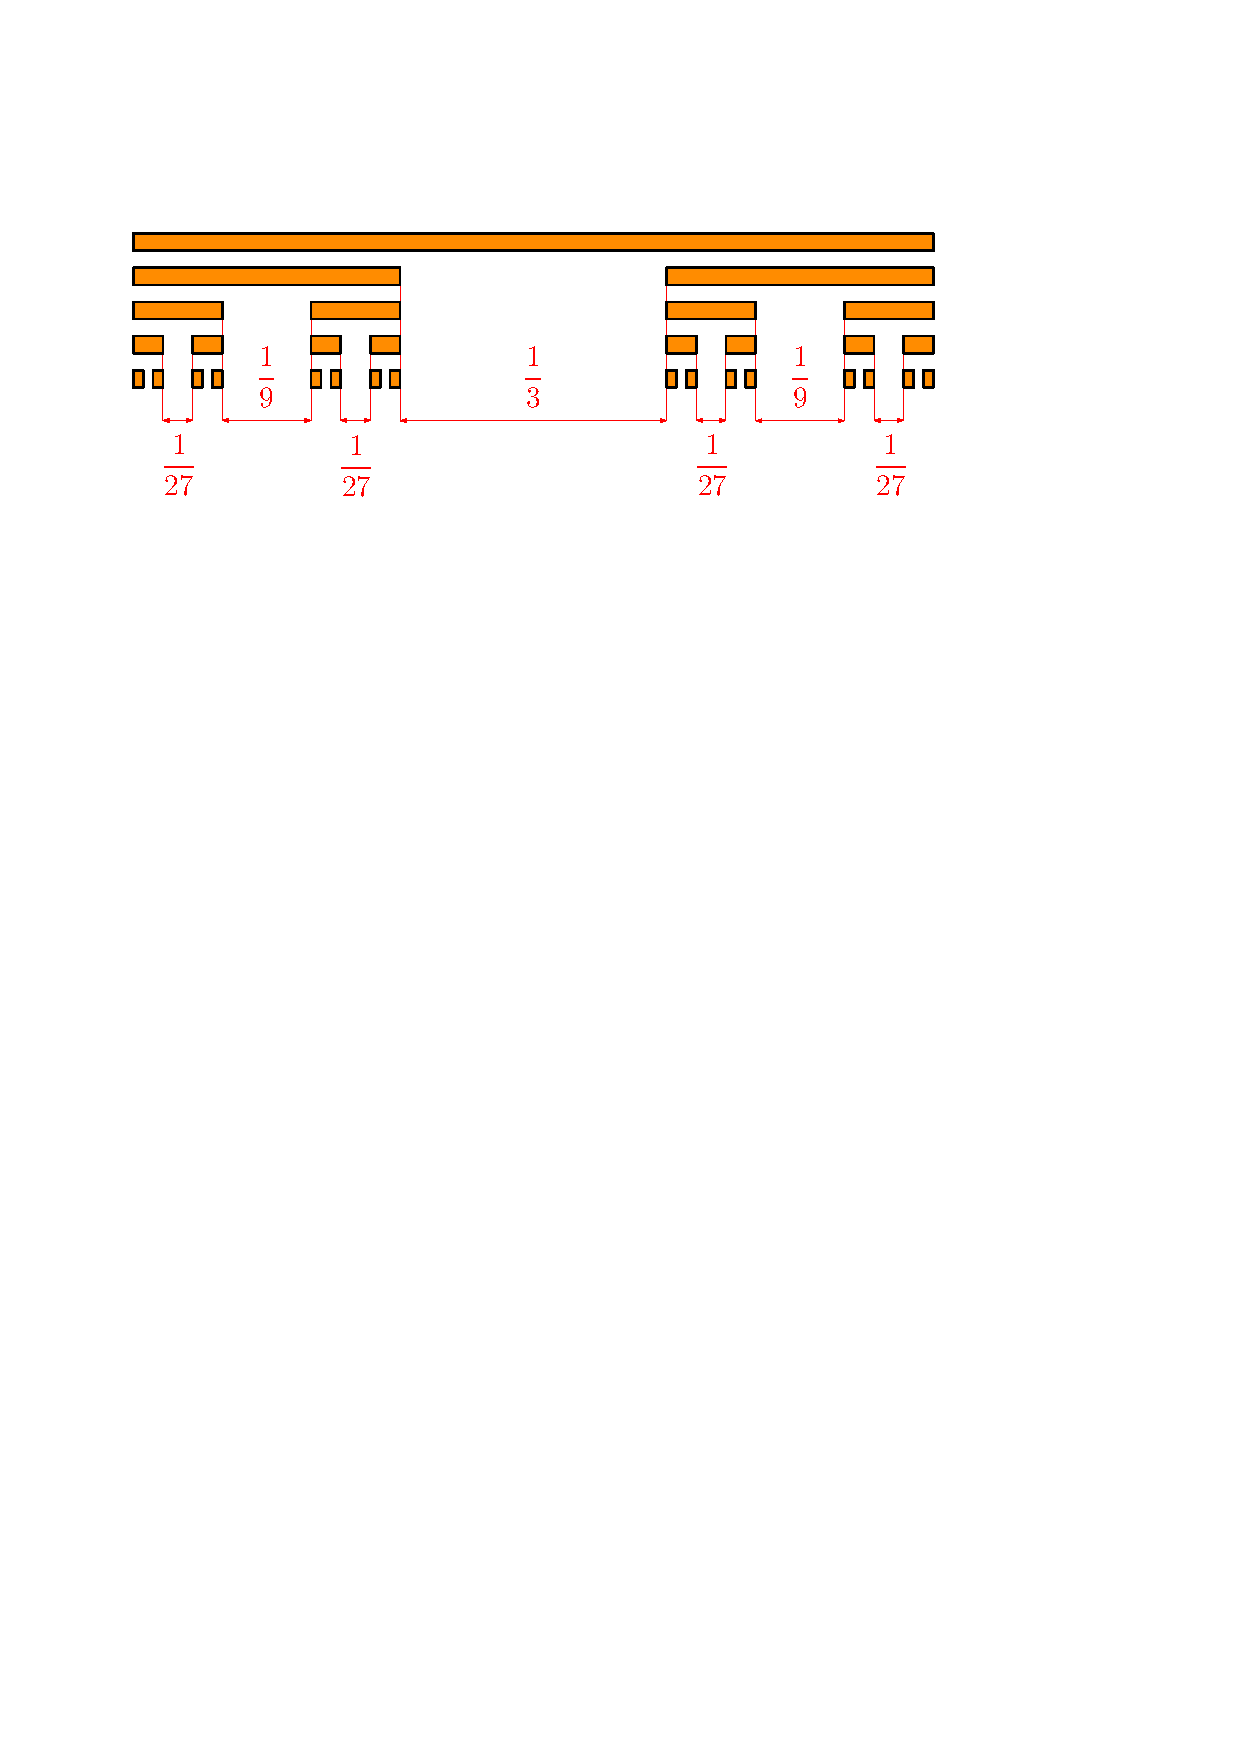
\includegraphics[scale=\normalipe]{ch01-cantorova-mnozina-delky.pdf}
    \caption{Znázornění délek vyjmutých úseků.}
    \label{fig:cantorovo_diskontinuum_delky}
\end{figure}
Obecně počet odebraných úseků roste s~mocninou dvojky,~jejichž délky klesají s~mocninou trojky,~tedy v~$n$-té iteraci odebereme úsek délky $2^n(1/3)^{n+1}$. Označíme-li tedy délku zbylých úseků $\ell_n$ po $n$ iteracích a $\overline{\ell_n}$ délku odebraných úseků,~pak určitě platí $\ell_n=1-\overline{\ell_n}$. Protože nás zajímá délka \emph{všech} odebraných úseků,~pak po $n$ iteracích bude celková délka rovna
\begin{equation}
    \overline{\ell_n}=\sum_{k=0}^{n}2^k\left(\dfrac{1}{3}\right)^{k+1}=\sum_{k=0}^{n}\dfrac{2^k}{3^{k+1}}=\dfrac{1}{3}\cdot\sum_{k=0}^{n}\left(\dfrac{2}{3}\right)^k=\dfrac{1}{3}\cdot\dfrac{1-\left(\dfrac{2}{3}\right)^{n+1}}{1-\dfrac{2}{3}}=1-\left(\dfrac{2}{3}\right)^{n+1}.
\end{equation}
Označíme-li si limitu výrazů posloupností $\ell_n$,~reps. $\overline{\ell_n}$,~jako $\ell$,~resp. $\overline{\ell}$,~pak dostaneme
\begin{equation*}
    \overline{\ell}=\lim_{n\to\infty}\overline{\ell_n}=\lim_{n\to\infty}\left(1-\left(\dfrac{2}{3}\right)^{n+1}\right)=1-\lim_{n\to\infty}\left(\dfrac{2}{3}\right)^{n+1}=1-0=1.
\end{equation*}
Z toho již triviálně plyne,~že
\begin{equation}
    \ell=\lim_{n\to\infty}\ell_n=\lim_{n\to\infty}(1-\overline{\ell_n})=1-\lim_{n\to\infty}\overline{\ell_n}=1-1=0,
\end{equation}
tzn. na konci procesu zbude Cantorovo diskontinuum délky nula.
\section{Fraktální dimenze}\label{sec:fraktalni_dimenze}

\subsection{Chápání konceptu dimenze}\label{subsec:koncept-dimenze}

Útvary vyčtené v~sekci~\ref{sec:sobepodobnost} ilustrují vlastnost soběpodobnosti,~kterou jsme si (zatím neformálně) popsali. V~eukleidovské geometrii lze však u~mnohých základních objektů pozorovat stejnou vlastnost. Např. čtverec lze určitě prohlásit v~jistém smyslu za soběpodobný,~neboť jej lze rozdělit na podobné útvary (viz obrázek~\ref{fig:sobepodobnost-ctverce}).
\begin{figure}[h]
    \centering
    \begin{subfigure}[b]{\subfigwidth}
        \centering
        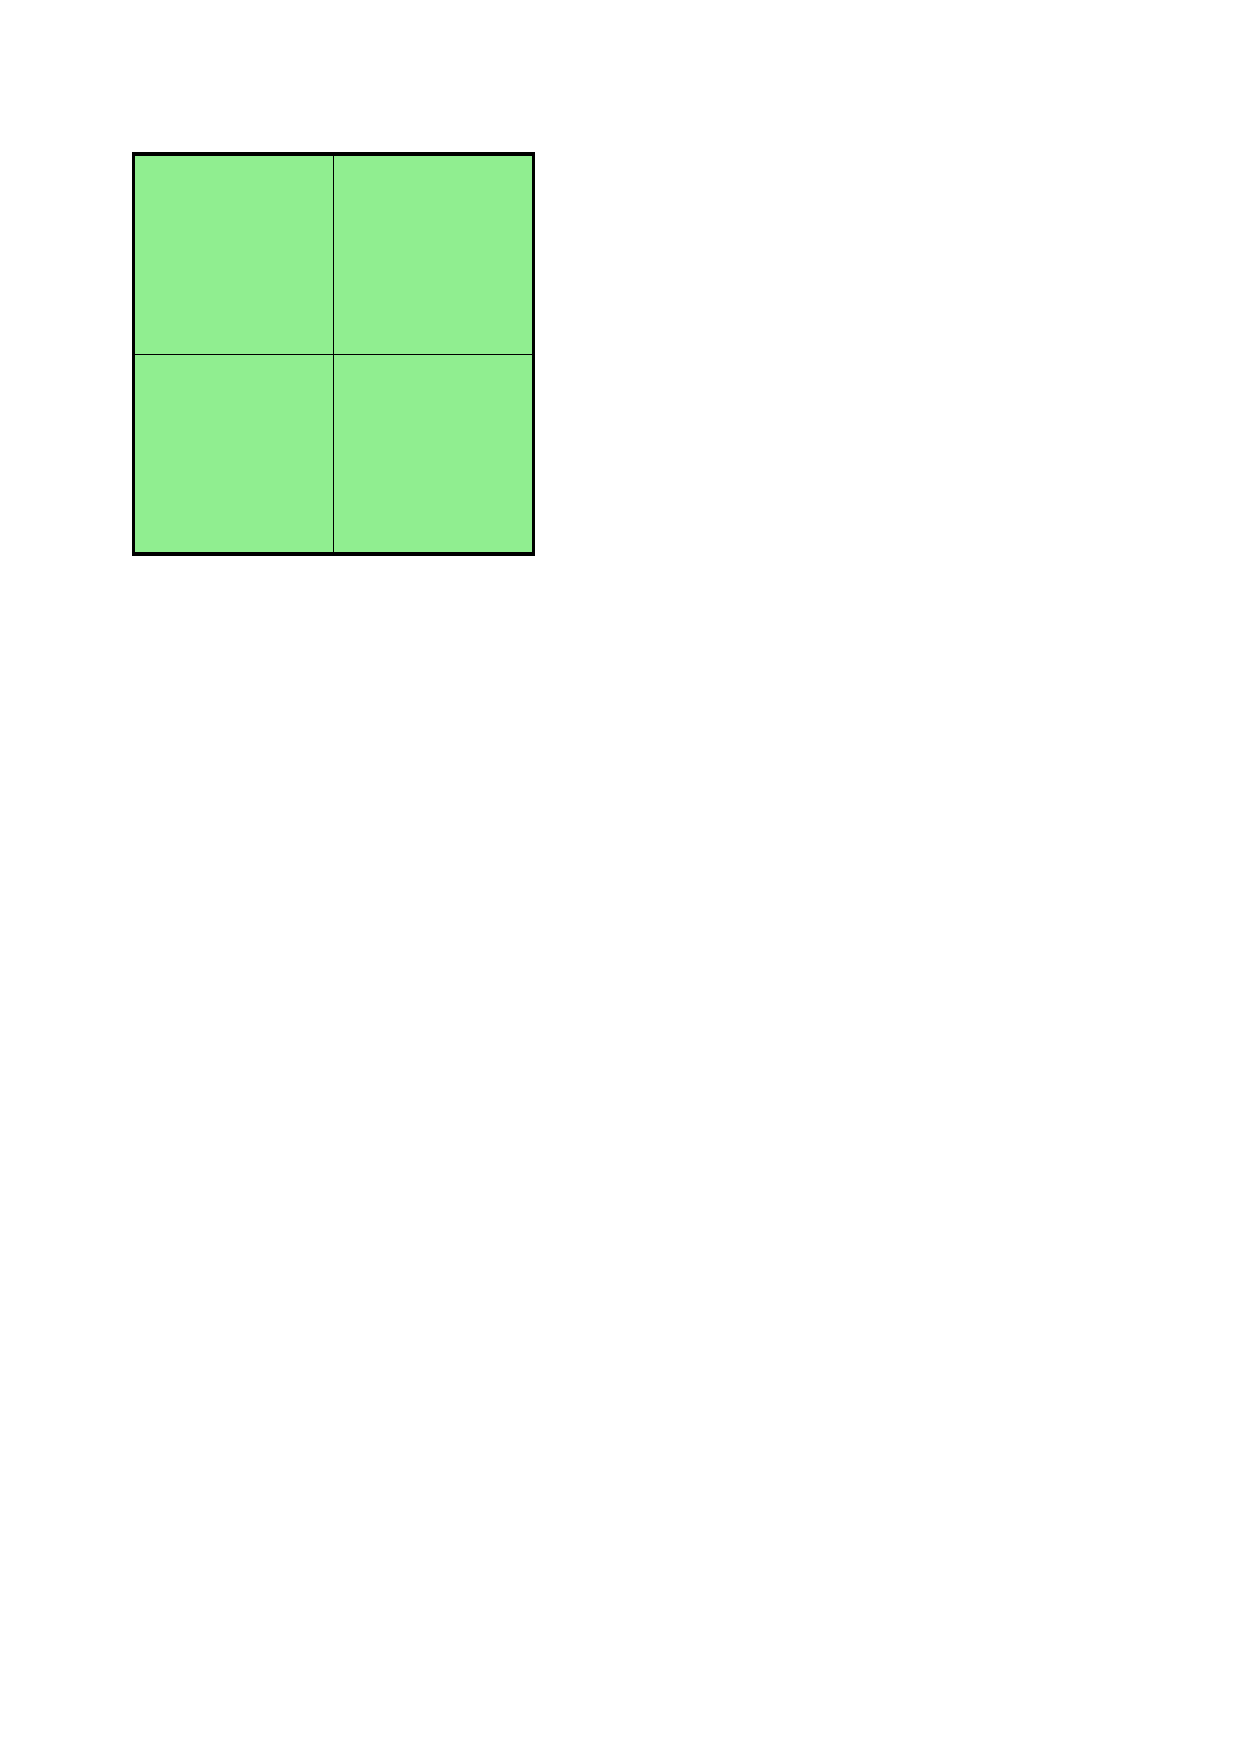
\includegraphics[scale=\normalipe]{ch01-ctverec-sobepodobnost.pdf}
        \caption{Rozdělení na čtyři menší čtverce.}
        \label{subfig:sobepodobnost-ctverce-1}
    \end{subfigure}
    \begin{subfigure}[b]{\subfigwidth}
        \centering
        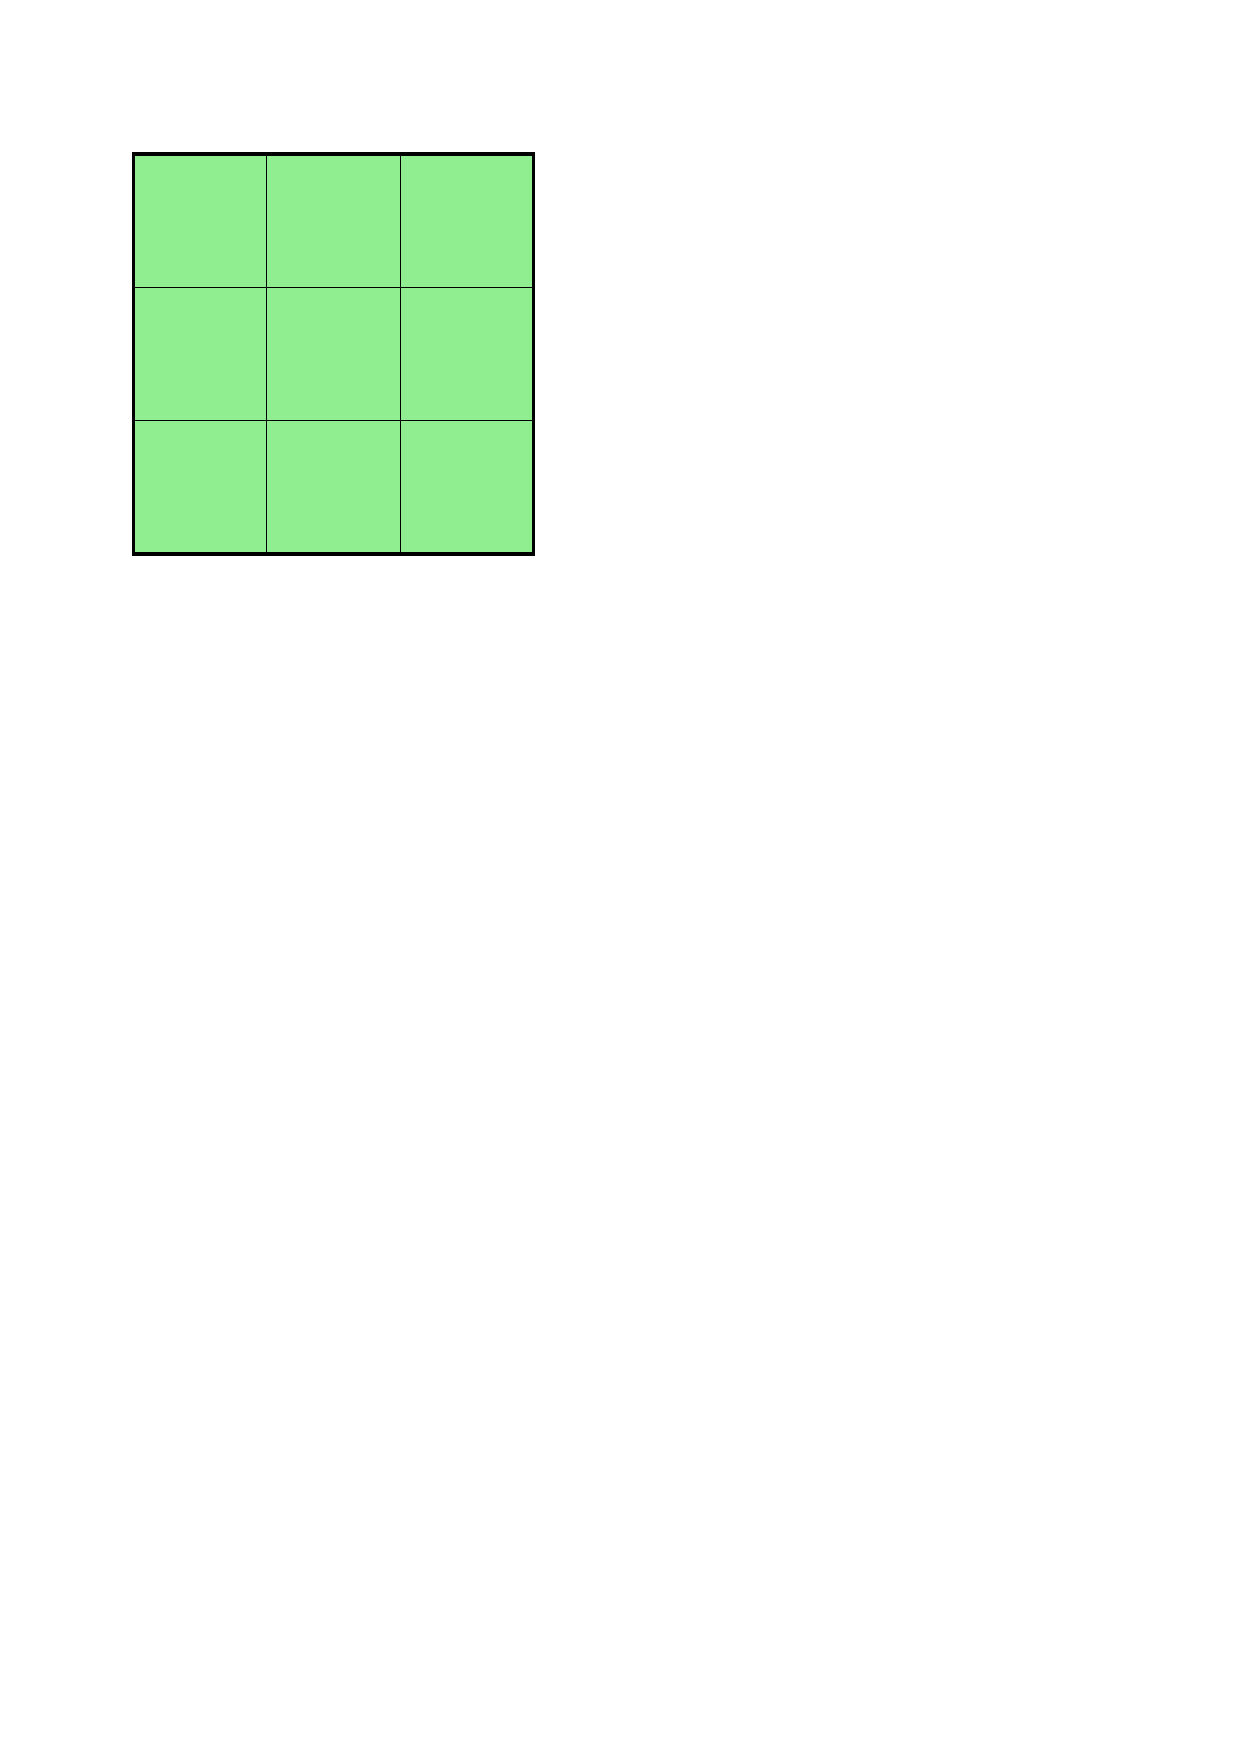
\includegraphics[scale=\normalipe]{ch01-ctverec-sobepodobnost-2.pdf}
        \caption{Jiná možnost rozdělení čtverce.}
        \label{subfig:sobepodobnost-ctverce-2}
    \end{subfigure}
    \caption{Soběpodobnost čtverce.}
    \label{fig:sobepodobnost-ctverce}
\end{figure}
Podobně např. i~obyčejná úsečka je taktéž soběpodobná,~protože ji můžeme rozdělit na $k$ stejných částí (viz obrázek~\ref*{fig:sobepodobnost-usecky}).\par
\begin{figure}[h]
    \centering
    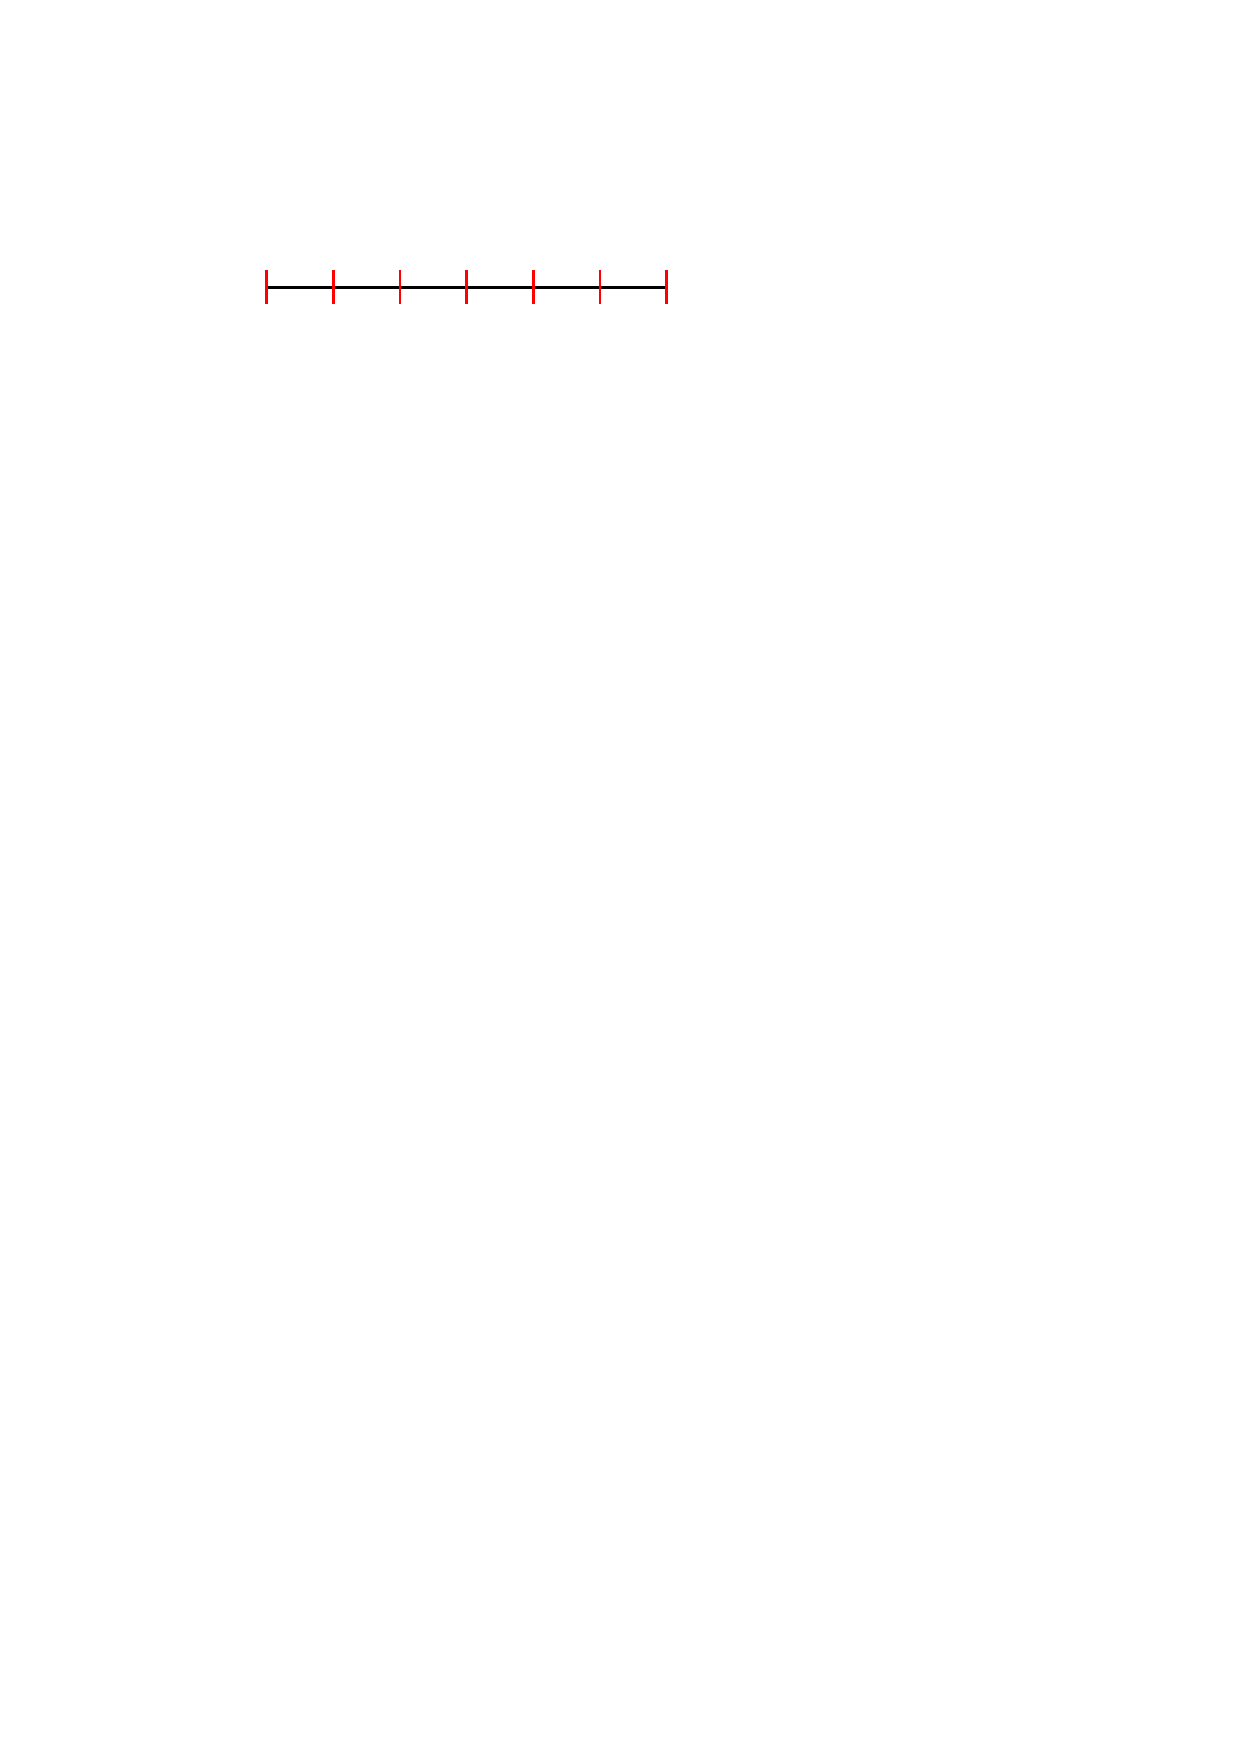
\includegraphics[scale=\normalipe]{ch01-usecka-sobepodobnost.pdf}
    \caption{Úsečka rozdělená na šest stejných částí.}
    \label{fig:sobepodobnost-usecky}
\end{figure}
K čemu nám takové uvědomění vlastně je? Zmenšíme-li úsečku $k$-krát,~pak budeme potřebovat přesně $k$ těchto částí,~abychom dostali úsečku původní délky. U~čtverce (nebo obdélníku obecně) při změnšení délky strany $k$-krát budeme potřebovat $k^2$ daných útvarů pro obdržení čtverce s~původním obsahem.\footnote{Obdélník zmenšený $k$-krát bude mít strany délek $a/k,\,b/k$,~tedy jeho obsah bude
\[\dfrac{ab}{k^2}=\dfrac{S}{k^2},\]
kde $S$ je obsah původního obdélníka.}
Pro krychli bude situace podobná,~$k$-krát zmenšená kopie bude potřeba $k^3$-krát,~abychom dostali krychli o~původním objemu (viz obrázek~\ref{fig:krychle-sobepodobnost}).
\begin{figure}[h]
    \centering
    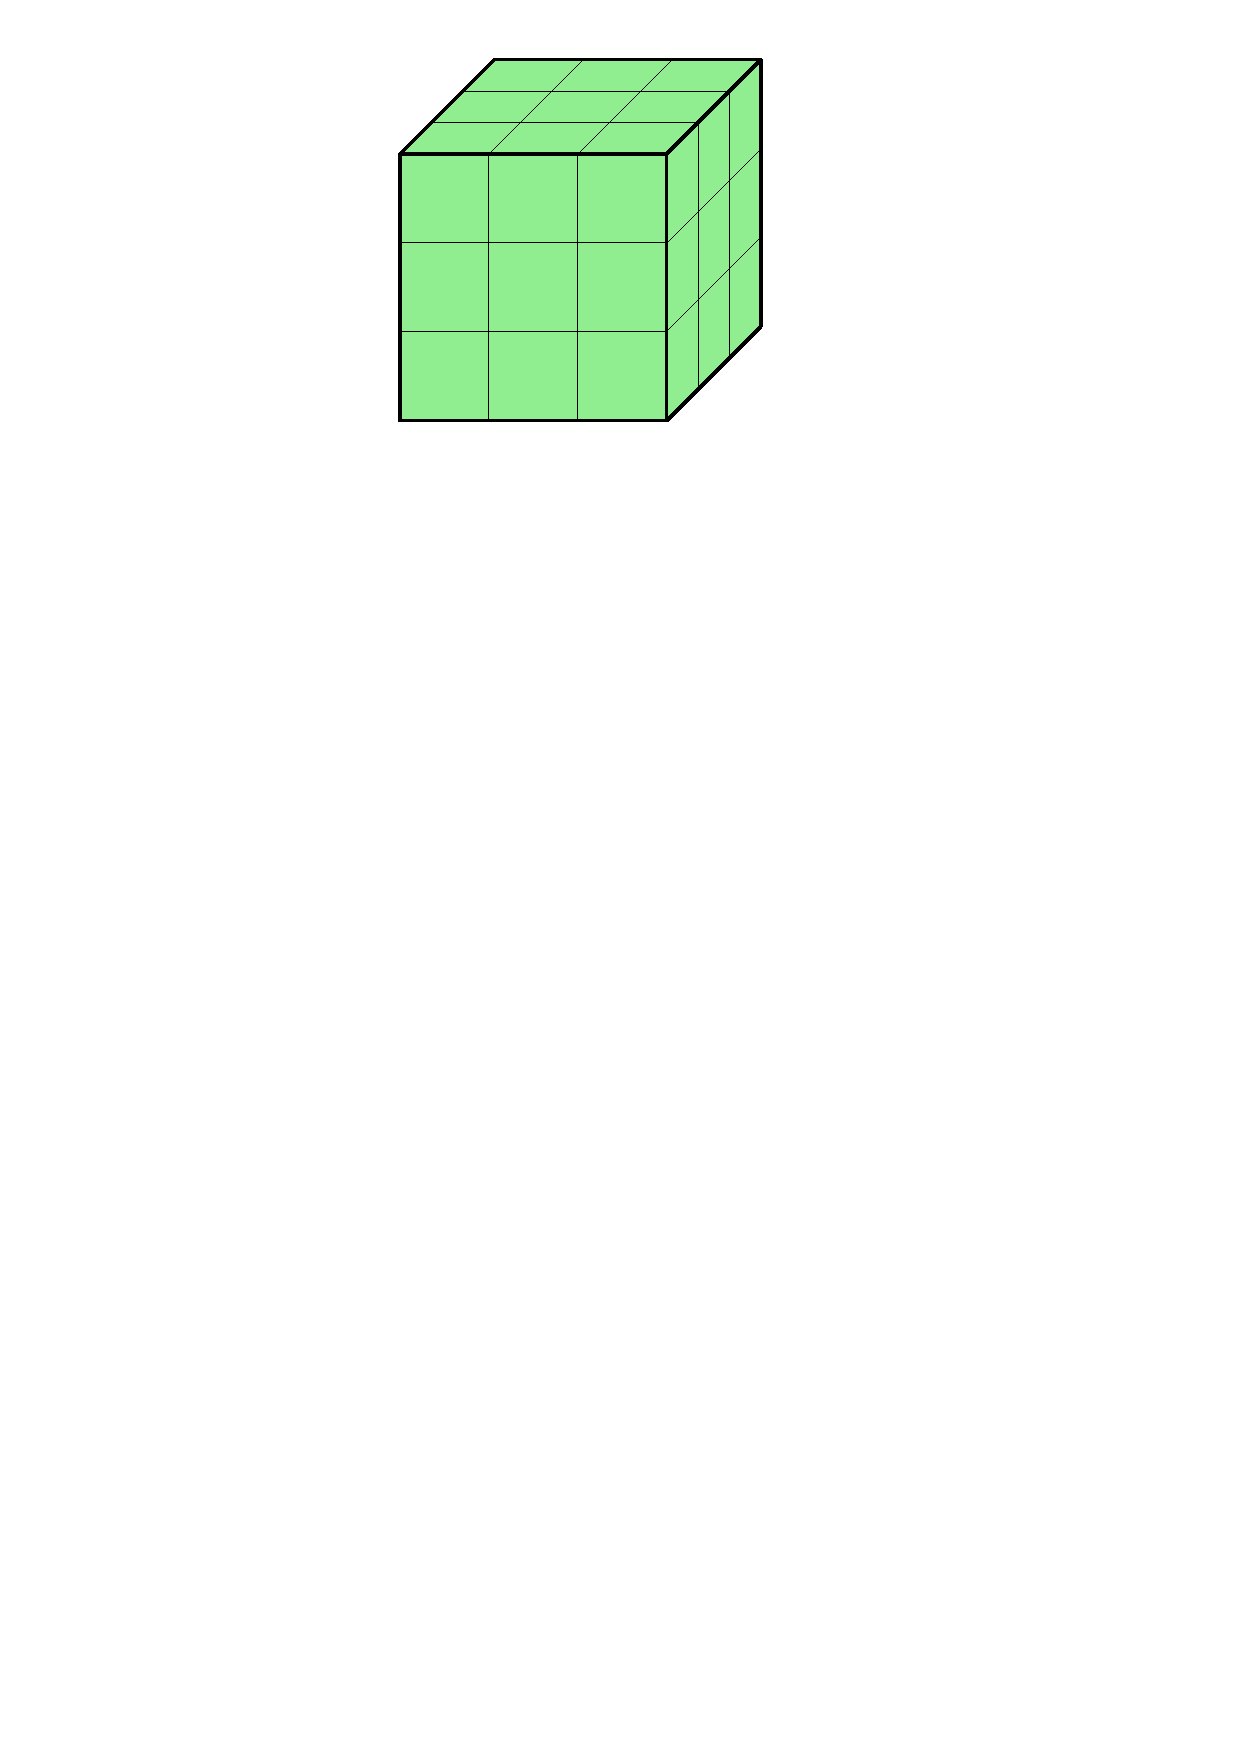
\includegraphics[scale=\normalipe]{ch01-krychle-sobepodobnost.pdf}
    \caption{Krychle rozdělená na 27 stejných částí.}
    \label{fig:krychle-sobepodobnost}
\end{figure}
Lze si všimnout,~že v~závislosti na \emph{dimenzi} objektu se mění daný exponent. Vztah lze tak zobecnit na
\begin{equation}\label{eq:pocet-utvaru}
    N(k)=k^d
\end{equation}
kde $N(k)$ je počet nových útvarů v~závislosti na faktoru $k$ a~číslu $d$. Intuitivně je nejspíše jasné,~že dimenze útvaru je takové číslo $d$,~pro které platí rovnost \eqref{eq:pocet-utvaru}.

Toto je jeden z~možných způsobů,~jak lze chápat koncept dimenze. Jednoduchou úpravou rovnosti \eqref{eq:pocet-utvaru} dostaneme
\[d=\log_k{N(k)}=\dfrac{\ln{N(k)}}{\ln{k}}.\]
(Obecně lze volit jakýkoliv přípustný základ logaritmů,~tj $d=\log_b{N(k)}/\log_b{k}$ pro $b\in\R_+\setminus\set{1}$.)

Dimenze v~tomto pojetí skutečně dává dobrý smysl. Pro "klasické" geometrické objekty vychází dimenze vždy celočíselně (viz tabulka \ref{table:eukleides-dimenze}).
\begin{table}[h]
    \centering
    \begin{tabular}{r|cc}
    Útvar    & $N(k)$ & $d=\ln{N(k)}/\ln{k}$ \\ \hline
    Úsečka   & $3$      & $1$                          \\
    Čtverec  & $9$      & $2$                          \\
    Krychle  & $27$     & $3$                          \\
    Teserakt & $81$     & $4$                          \\
    \end{tabular}
    \caption{Hodnoty dimenze $d$ pro různé útvary.}
    \label{table:eukleides-dimenze}
\end{table}

Na této myšlence je založen pojem tzv. \emph{fraktální dimenze}\index{fraktální dimenze}\index{dimenze!fraktální}. Existuje více neekvivalentních způsobů její definice. Jedna z~nich,~které se dále nyní v~této sekci budeme držet,~se v~anglicky psané literatuře nazývá \emph{"box-counting dimension"}\index{box-counting dimenze}\index{dimenze!box-counting},~odkud plyne i~značení $\dimB$. Pro útvar $F$ (formálně vzato množinu bodů) definujeme 
\begin{equation}\label{eq:fraktalni-dimenze}
    \dimB{F}=\lim_{\varepsilon\to 0_+}{\dfrac{\ln{N_\varepsilon(F)}}{\ln{\left(\frac{1}{\varepsilon}\right)}}}.
\end{equation}
(Převzato z~\cite[str. 93]{Zelinka2006} a~\cite[str. 28]{Falconer2014}.) Výraz $1/\varepsilon$ zde představuje faktor podobnosti jako původní $k$ (samotné $\varepsilon$ tak hraje roli měřítka). Číslo $N_\varepsilon(F)$ je počet soběpodobných útvarů,~na které jsme rozdělili původní útvar $F$ v měřítku $\varepsilon$. Největší rozdíl zde však představuje zkoumání "limitního chování" daného výrazu.

Nejdříve poznamenejme, pro "klasické" geometrické útvary hodnota $\dimB{F}$ vychází skutečně tak, jak jsme zvyklí. Toto si ilustrujeme na příkladech~\ref{ex:fraktalni-dimenze-usecka},~\ref{ex:fraktalni-dimenze-ctverec} a~\ref{ex:fraktalni-dimenze-trojuhelnik}.
\begin{example}[Fraktální dimenze úsečky]\label{ex:fraktalni-dimenze-usecka}
    Začněme asi nejednodušším příkladem výpočtu fraktální dimenze,~a to u~úsečky (označme $\ell$). Představme si,~že úsečku \emph{jednotkové délky} rozdělíme na $N_\varepsilon(\ell)=n$ shodných dílů. Pak měřítko libovolného dílu je
    \[\varepsilon=\dfrac{1}{n}=n^{-1}.\]
    (Zde je dobré si uvědomit,~že pro $n\to\infty$,~tedy zjemňování dělení úsečky,~platí,~že $\varepsilon\to 0_+$.) Fraktální dimenzi úsečky vypočteme z~definice jako
    \[\dimB{\ell}=\lim_{\varepsilon\to 0_+}{\dfrac{\ln{N_\varepsilon(\ell)}}{\ln{\left(\frac{1}{\varepsilon}\right)}}}=\lim_{n\to\infty}{\dfrac{\ln{n}}{\ln{n}}}=1.\]
\end{example}
\begin{example}[Fraktální dimenze čtverce]\label{ex:fraktalni-dimenze-ctverec}
    Podobně,~jako v~příkladu~\ref{ex:fraktalni-dimenze-usecka}\linebreak{}výše,~můžeme stanovit i~fraktální dimenzi čtverce (označme $S$). Uvažujme tedy čtverec o~jednotkovém obsahu,~který rozdělíme $N_\varepsilon(S)=n$ shodných útvarů. Přitom víme,~že obsah mění kvadraticky vůči délce strany. Měřítko nového čtverce tak bude
    \[\varepsilon=\sqrt{\dfrac{1}{n}}=n^{-1/2}\]
    a~fraktální dimenze vychází
    \[\dimB{S}=\lim_{n\to\infty}{\dfrac{\ln{n}}{\ln{n^{1/2}}}}=\lim_{n\to\infty}{\dfrac{\ln{n}}{\frac{1}{2}\ln{n}}}=2.\]
\end{example}
Pro krychli bude výpočet naprosto analogický (viz příklad~\ref{ex:fraktalni-dimenze-ctverec}). Obecně pro $d$-rozměrnou krychli bude její fraktální dimenze\footnote{Obdobnou úvahou dojmeme k~měřítku $\varepsilon=n^{-1/d}$.} rovna $d$.\par
Zkusme se nyní oprostit od krychle k~trochu jinému útvaru.
\begin{example}[Fraktální dimenze trojúhelníka]\label{ex:fraktalni-dimenze-trojuhelnik}
    Podívejme se,~jak to dopadne s~fraktální dimenzí \emph{obecného trojúhelníku}. Každý trojúhelník $T$ lze rozdělit na čtveřici \emph{vzájemně shodných trojúhelníků $T_1,\dots,T_4$},~které vzniknou sestrojením středních příček v~původním trojúhelníka (viz obrázek~\ref{fig:trojuhelnik-sobepodobnost}).
    \begin{figure}[h]
        \centering
        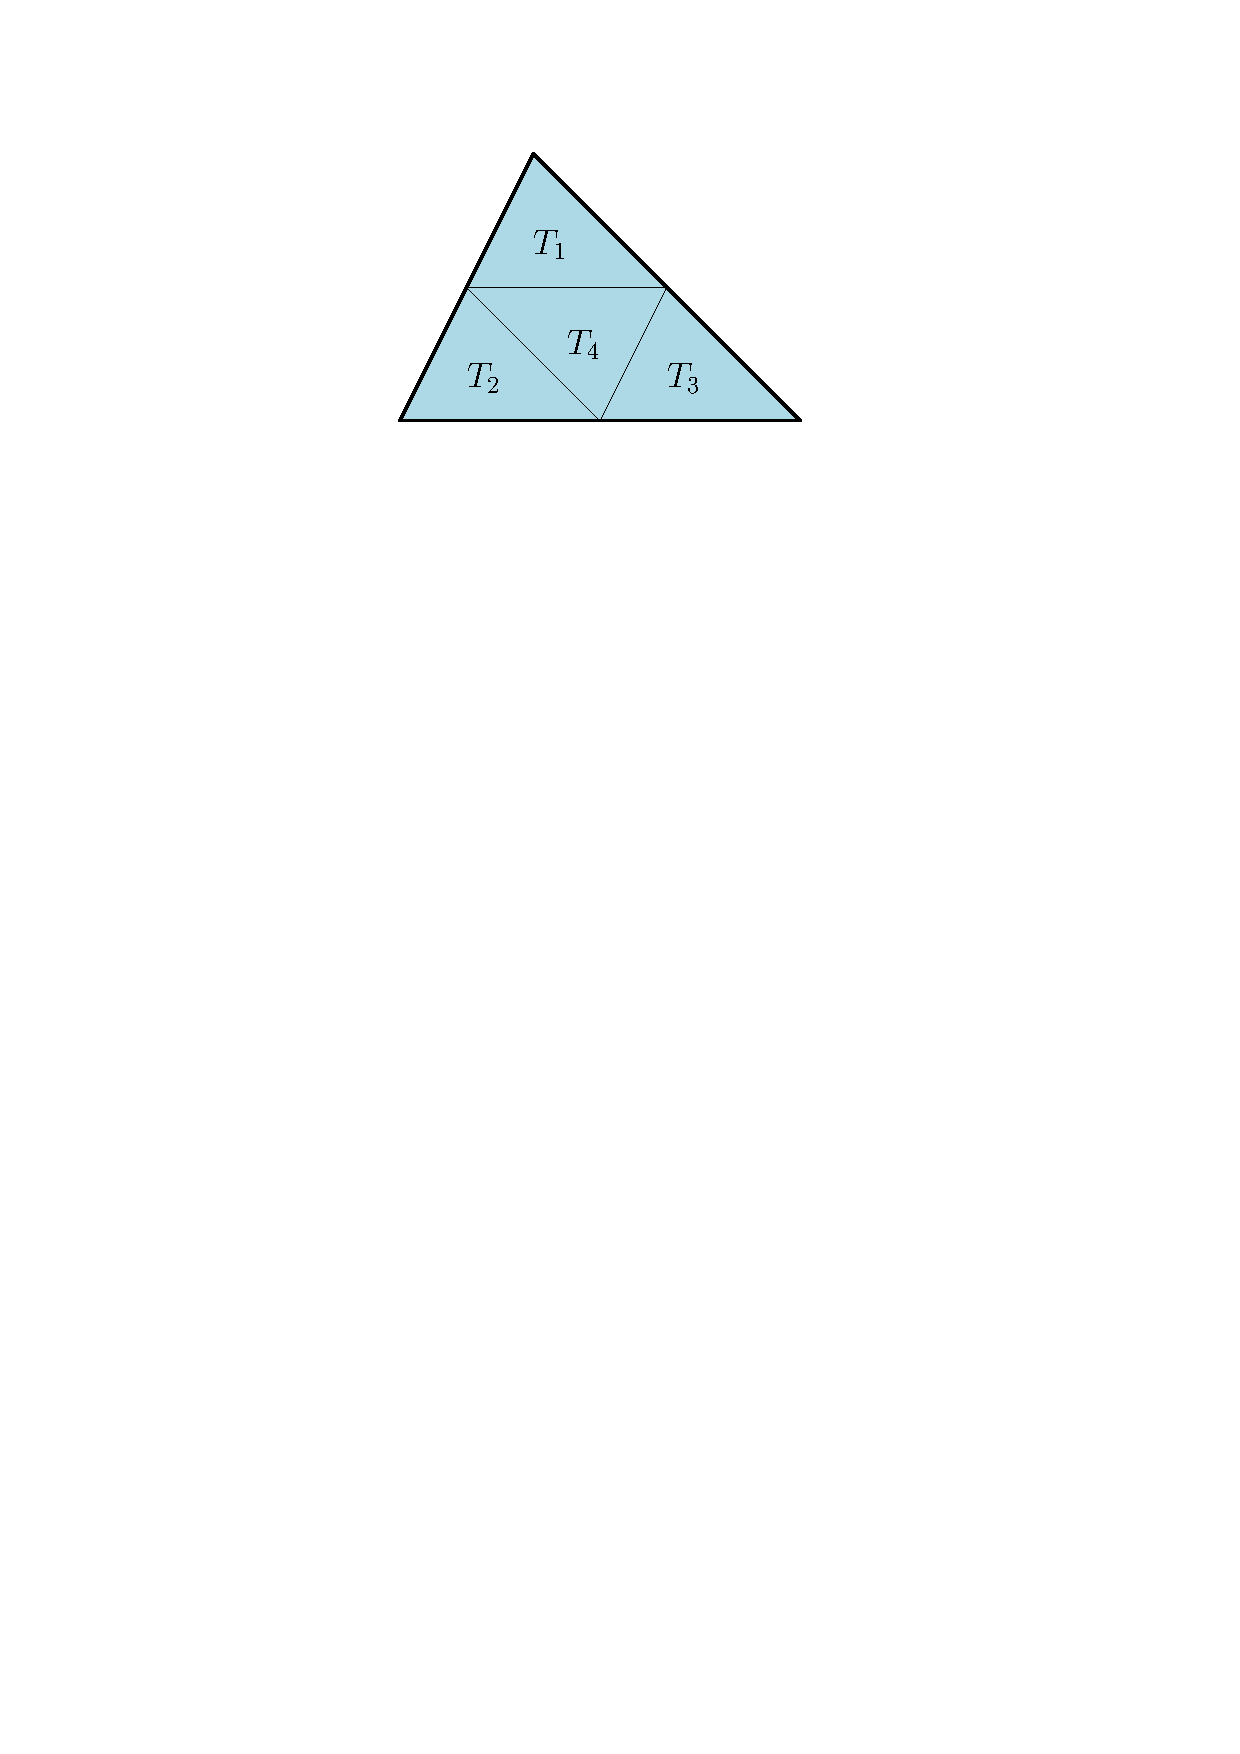
\includegraphics[scale=\normalipe]{ch01-trojuhelnik-sobepodobnost.pdf}
        \caption{Trojúhelník $T$ rozdělený na trojúhelníky $T_1,\dots,T_4$.}
        \label{fig:trojuhelnik-sobepodobnost}
    \end{figure}
    Délka každé střední příčky odpovídá polovině délky strany,~s~níž je rovnoběžná,~tedy obsah každého z~menších trojúhelníků je \emph{čtvrtina obsahu původního} trojúhelníka $T$. Tento postup můžeme opakovat pro každý z menších trojúhelníků, čímž dostaneme $4^2$ trojúhelníků. Takto můžeme postupovat libovolně dlouho,~přičemž po $n$ krocích bude počet\footnote{Výpočet bychom mohli i~zde provést ve stejném duchu jako u~úsečky,~čtverce nebo krychle. Počet částí,~na než rozdělíme trojúhelník,~označíme $N_\varepsilon(T)=n$,~přičemž měřítko pak bude $\varepsilon=n^{-1/2}$.} vzniklých trojúhelníků $N_\varepsilon(T)=4^n$,~přičemž měřítko každého z~nich bude $\varepsilon=(1/2)^n$. Fraktální dimenze tak vychází:
    \[\dimB{T}=\lim_{n\to\infty}{\dfrac{\ln{4^n}}{\ln{2^n}}}=\lim_{n\to\infty}{\dfrac{2n\ln{2}}{n\ln{2}}}=2.\]
\end{example}
Pro jednoduché útvary vychází dimenze tak,~jak bychom mohli očekávat. K~zajímavějším výsledkům však dospějeme u~fraktálů,~na něž se blíže podíváme v~následující podsekci~\ref{subsec:dimenze-fraktalu}.

\subsection{Dimenze fraktálů}\label{subsec:dimenze-fraktalu}

Co kdybychom však zkusili podobnou myšlenku aplikovat i~na \emph{fraktální objekty} jako např. Kochovu křivku, Kochovu vločku, Sierpińského trojúhelník nebo Cantorovo diskontinuum? Zkusme to. Pro připomenutí jednotlivých křivek a~výsledků k~nim si dovoluji čtenáře opětovně odkázat na sekci~\ref{sec:sobepodobnost},~kde jsou podrobněji rozebrány.

V tomto případě uvidíme,~že dochází na první pohled k~docela zvláštnímu jevu. Fraktální dimenze již totiž nemusí vycházet celočíselně,~jak jsme zvyklí.
\begin{itemize}
    \item \textbf{Kochova křivka $F_{KC}$.} V~každé iteraci nahrazujeme každou úsečku čtyřmi novými. Kompletní Kochova křivka tak obsahuje právě \emph{čtyři} kopie sebe sama zmenšené na třetinu,~tj. v~$n$-té iteraci je $N_\varepsilon(F_{KC})=4^n$,~jak jsme již odvodili (viz podsekce~\ref{subsec:kochova_krivka}).\footnote{Lze však zvolit i~jiné dělení. Např. lze na Kochovu křivku nahlížet,~že obsahuje \emph{16 kopií} sebe sama zmenšených na \emph{devítinu}.} Měřítko nově vzniklých částí je tak $\varepsilon=(1/3)^n$.
    \begin{equation}\label{eq:kochova-krivka-dimenze}
        \dimB{F_{KC}}=\lim_{\varepsilon\to 0_+}{\dfrac{\ln{N_\varepsilon(F_{KC})}}{\ln{\left(\frac{1}{\varepsilon}\right)}}}=\lim_{n\to\infty}{\dfrac{\ln{4^n}}{\ln{3^n}}}=\dfrac{\ln{4}}{\ln{3}}\approx 1{,}2618595\dots
    \end{equation}
    \item \textbf{Kochova vločka $F_{KS}$.} Začínáme s~rovnostranným trojúhelníkem o~straně délky $1$,~na jehož stranách postupně vznikne Kochova křivka. V~$n$-té iteraci je obvod Kochovy vločky $o_n$ roven $3\cdot 4^n$,~tj. i~$N_\varepsilon(F_{KS})=3\cdot 4^n$,~kde měřítko\footnote{Měřítko se ve srovnání s~Kochovou křivkou liší v~mocnině,~neboť délku nových úseků porovnáváme s~obvodem celého trojúhelníka,~nikoliv pouze délkou jedné jeho strany. Nicméně ve výpočtu bychom se mohli omezit i~jen na jednu ze stran,~výpočet by byl tak zcela identický jako u~Kochovy křivky.} nově vzniklých úseček je $\varepsilon=1/3\cdot(1/3)^n=(1/3)^{n+1}$. Není těžké se přesvědčit,~že fraktální dimenze vychází stejně,~jako u~Kochovy křivky:
    \begin{equation}\label{eq:kochova-vlocka-dimenze}
        \dimB{F_{KS}}=\lim_{n\to\infty}{\dfrac{\ln{3\cdot 4^n}}{\ln{3^{n+1}}}}=\lim_{n\to\infty}{\dfrac{\ln{4^n}\overbrace{\left(1+\frac{\ln{3}}{\ln{4^n}}\right)}^{\to 1}}{\ln{3^n}\underbrace{\left(1+\frac{\ln{3}}{\ln{3^n}}\right)}_{\to 1}}}=\dfrac{\ln{4}}{\ln{3}}
    \end{equation}
    \item \textbf{Sierpińského trojúhelník $F_{ST}$.} V~každé iteraci vynecháme prostřední trojúhelník,~čímž vznikne \emph{trojice} nových trojúhelníků s~\emph{polovičním} měřítkem. Tzn.~$N_\varepsilon(F_{ST})=3^n$ pro $\varepsilon=(1/2)^n$,~a tedy
    \begin{equation}\label{eq:sierpinskeho-trojuhelnik-dimenze}
        \dimB{F_{ST}}=\lim_{n\to\infty}{\dfrac{\ln{3^n}}{\ln{2^{n}}}}=\dfrac{\ln{3}}{\ln{2}}\approx 1{,}5849625\dots
    \end{equation}
    \item \textbf{Cantorovo diskontinuum $F_{CD}$.} Vždy vyjmeme prostřední třetinu\linebreak{}úsečky,~čímž obdržíme \emph{dvojici} úseček \emph{třetinové} délky,~tj. $N_\varepsilon(F_{CD})=2^n$ pro $\varepsilon=(1/3)^n$. Fraktální dimenze tak vychází
    \begin{equation}\label{eq:cantorovo-diskontinuum-dimenze}
        \dimB{F_{CD}}=\lim_{n\to\infty}{\dfrac{\ln{2^n}}{\ln{3^n}}}=\dfrac{\ln{2}}{\ln{3}}\approx 0{,}6309297\dots
    \end{equation}
\end{itemize}
Udělejme si nyní menší souhrn a~porovnání dosud získaných výsledků (viz tabulka~\ref{table:fraktaly-eukleides-dimenze}).
\begin{table}[h]
    \centering
    \begin{tabular}{r|ccc}
        Útvar $F$                & $\varepsilon$ & $N_\varepsilon(F)$ & $\dimB{F}$         \\ \hline
        Úsečka                   & $n^{-1}$      & $n$                & 1                  \\
        Čtverec                  & $n^{-1/2}$    & $n$                & 2                  \\
        Krychle                  & $n^{-1/3}$    & $n$                & 3                  \\
        Teserakt                 & $n^{-1/4}$    & $n$                & 4                  \\
        $d$-rozměrná krychle     & $n^{-1/d}$    & $n$                & $d$                \\
        Obecný trojúhelník       & $(1/2)^n$     & $4^n$              & 2                  \\
        Kochova křivka           & $(1/3)^n$     & $4^n$              & $1{,}2618595\dots$ \\
        Kochova vločka           & $(1/3)^{n+1}$ & $3\cdot 4^n$       & $1{,}2618595\dots$ \\
        Sierpińského trojúhelník & $(1/2)^n$     & $3^n$              & $1{,}5849625\dots$ \\
        Cantorovo diskontinuum   & $(1/3)^n$     & $2^n$              & $0{,}6309297\dots$ \\
    \end{tabular}
    \caption{Porovnání fraktálních dimenzí $d_k$ různých objektů.}
    \label{table:fraktaly-eukleides-dimenze}
\end{table}
Můžeme si všimnout,~že zatímco u~"klasických" objektů vychází fraktální dimenze \emph{celočíselná},~u~(zmíněných) fraktálů vychází \emph{neceločíselně},~ba dokonce i~iracionálně.

\subsection{Topologická dimenze}\label{subsec:topologicka-dimenze}

Výsledky z~předešlé části~\ref{subsec:dimenze-fraktalu} se můžou zdát poněkud překvapující. Jak je vůbec možné,~že dimenze nemusí vycházet nutně celočíselná? Ač se to možná zdá jako nesmyslný výsledek,~je třeba si uvědomit,~jak vlastně koncept dimenze chápeme. Na jednu stranu na ni lze nahlížet jako na mocninu "s níž se zvyšuje" obsah/objem tělesa, měníme-li měřítko. Naopak čtenář znalý lineární algebry si možná vzpomene,~že v~této matematické disciplíně se na dimenzi nahlíží jako na \emph{mohutnost libovolné báze daného vektorového prostoru},~která naopak vychází vždy pouze celočíselně, případně nekonečná,~avšak nelze s~ní dobře zachytit hlubší detail geometrie u~objektů,~jako jsou právě fraktály.

Dalším možným pojetím pojmu dimenze nám dává tzv. \emph{topologická dimenze}\index{dimenze!topologická}\index{topologická dimenze}. Ty totiž daleko více odpovídají našemu intuitivnímu chápání tohoto pojmu,~neboť se vždy jedná o~celé číslo,~jak ho známe ze školní geometrie. Existuje více topologických dimenzí\footnote{Jiným příkladem takové dimenze je \emph{induktivní dimenze}.},~které si,~co do definice,~obecně nejsou ekvivalentní,~ačkoliv ve většině standardních případů splývají. My se zde pro ilustraci podíváme na tzv. \emph{Lebesgueovu pokrývací dimenzi}\index{dimenze!Lebesgueova pokrývací}\index{Lebesgueova pokrývací dimenze} (dále jen již "topologickou dimenzi") pojmenovanou po francouzském matematikovi \name{Henri Lebesgueovi}\index{Henri Lebesgue} (1875--1941). Myšlenka definice je založena na pokrývání objektu (formálně vzato \emph{množiny bodů}) tzv. \emph{otevřenými množinami}\index{množina!otevřená}\index{otevřená množina}.\footnote{Otevřená množina je zobecnění pojmu otevřeného intervalu reálných čísel. Neformálně řečeno je to taková množina $X$,~kde pro každý její bod $x\in X$ patří do této množiny i~nějaké $\varepsilon$-okolí tohoto bodu (patří do ní i~body,~které jsou "dostatečně blízko").} Formální definici si zde v~rámci zachování jednoduchosti odpustíme,~avšak pro hlubší matematický základ si dovolím čtenáře odkázat např. na knihu \cite{Engelking1989}. Avšak pokusíme se ji alespoň nastínit.

Množina $X$ má topologickou dimenzi $\dimL{X}=n$,~pokud $n$ je nejmenší číslo,~takové,~že pro každé pokrytí otevřenými množinami\footnote{Formálněji to znamená,~že $A_1,\dots,A_n$ jsou otevřené množiny,~takové,~že platí $X\subseteq\bigcup_{i=1}^n{A_i}$.} $\mathcal{U}$ existuje zjemnění\footnote{Zjemněním pokrytí $\mathcal{U}$ nazýváme takové pokrytí $\mathcal{U}^\prime$ množiny $X$,~kde každá množina $A_i^\prime\in\mathcal{U}^\prime$ je \emph{podmnožinou} nějaké množiny $A_j$ původního pokrytí $\mathcal{U}$.}\index{zjemnění} $\mathcal{U}^\prime$ takové,~že každý bod $x\in X$ náleží nejvýše $n+1$ množin pokrytí $\mathcal{U}$.

% Obecně množina $X$ má topologickou dimenzi $\dimL{X}=n$,~pokud danou množinu nelze pokrýt\footnote{Formálněji to znamená,~že $A_1,\dots,A_n$ jsou otevřené množiny,~takové,~že platí $X\subseteq\bigcup_{i=1}^n{A_i}$.} lib. otevřenými množinami,~tak,~že pro každé zjemnění $\mathcal{U}$ tohoto pokrytí platí,~že každý jeho bod $x$ je obsažen v~průniku nejvýše $n+1$ množin $\mathcal{U}$.

Tuto ideu si zkusíme přiblížit na příkladu topologické dimenze úsečky (viz obrázek~\ref{fig:usecka-zjemneni}).
\begin{figure}[h]
    \centering
    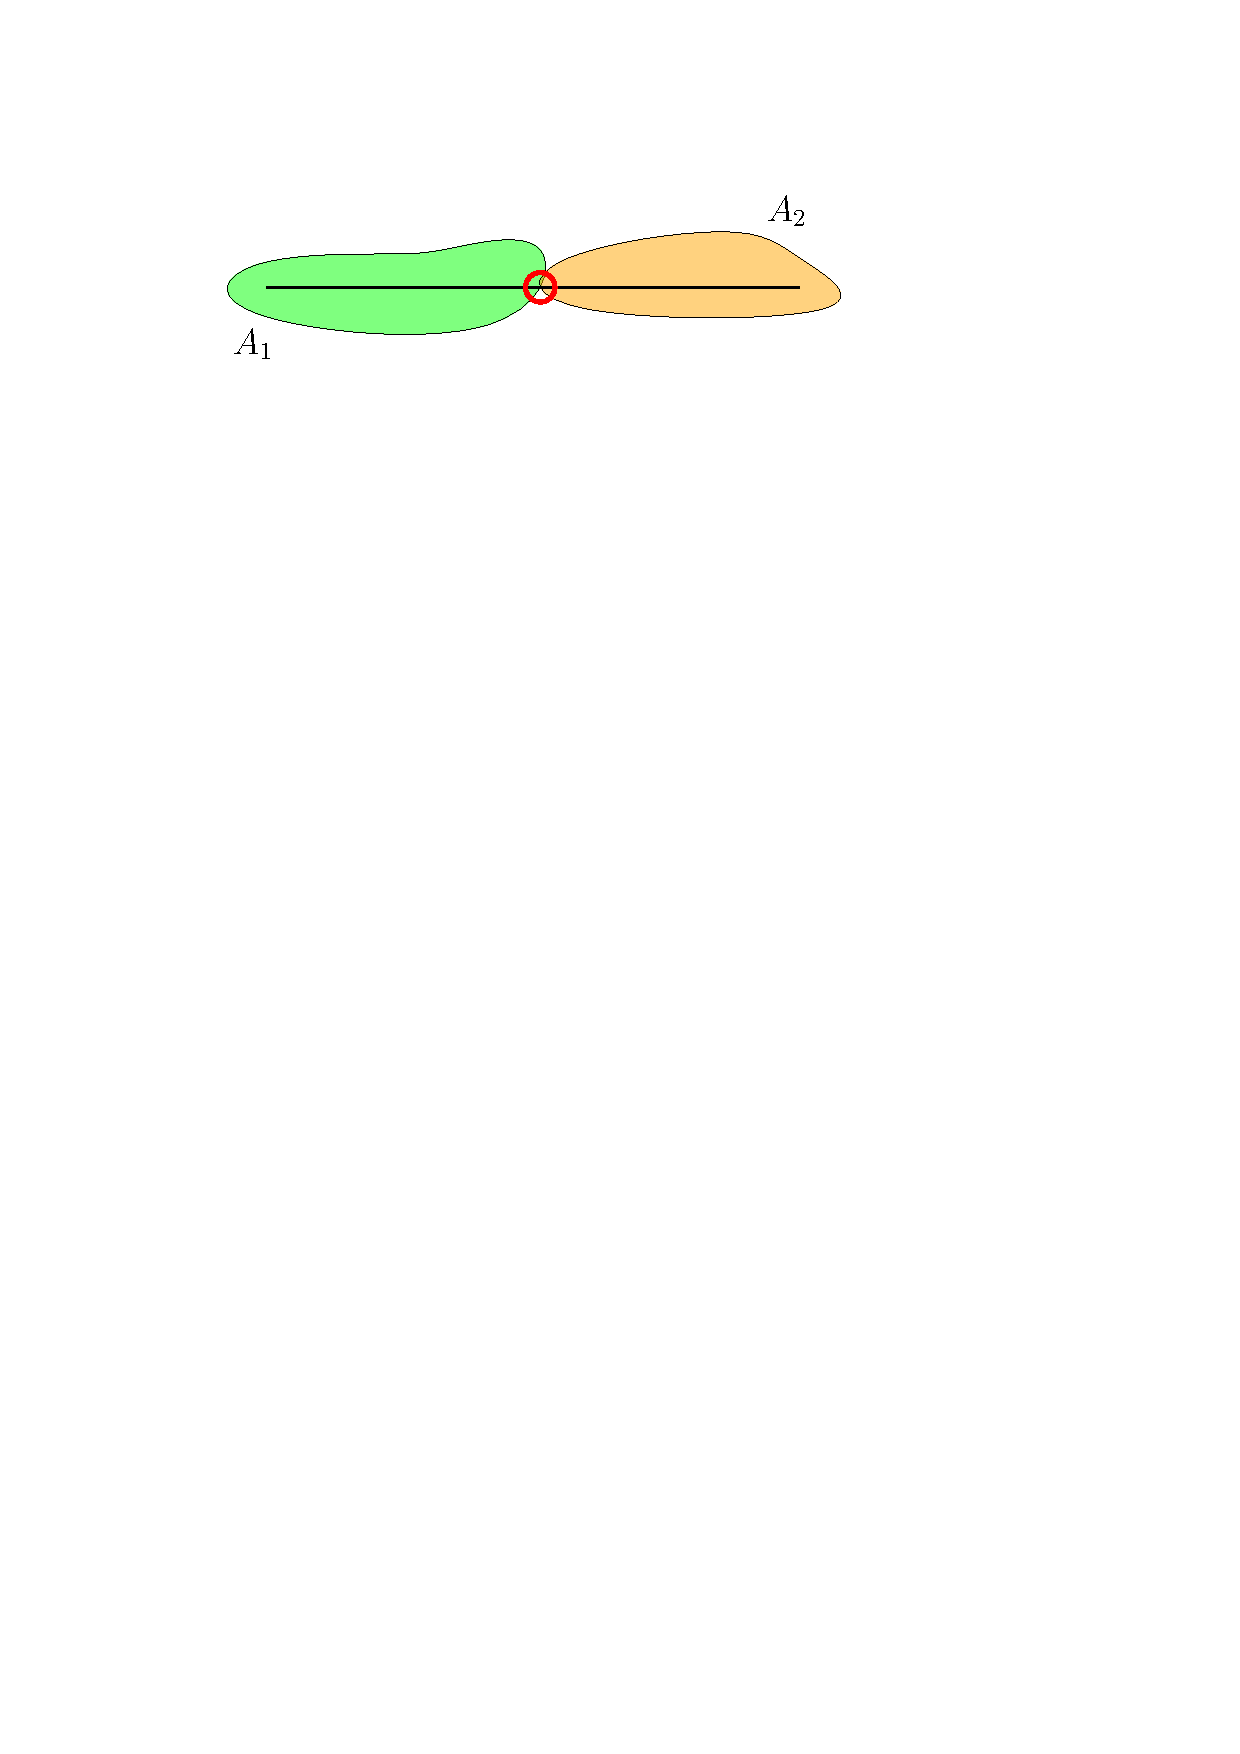
\includegraphics[scale=\normalipe]{ch01-usecka-pokryti-1.pdf}\\\qquad\\
    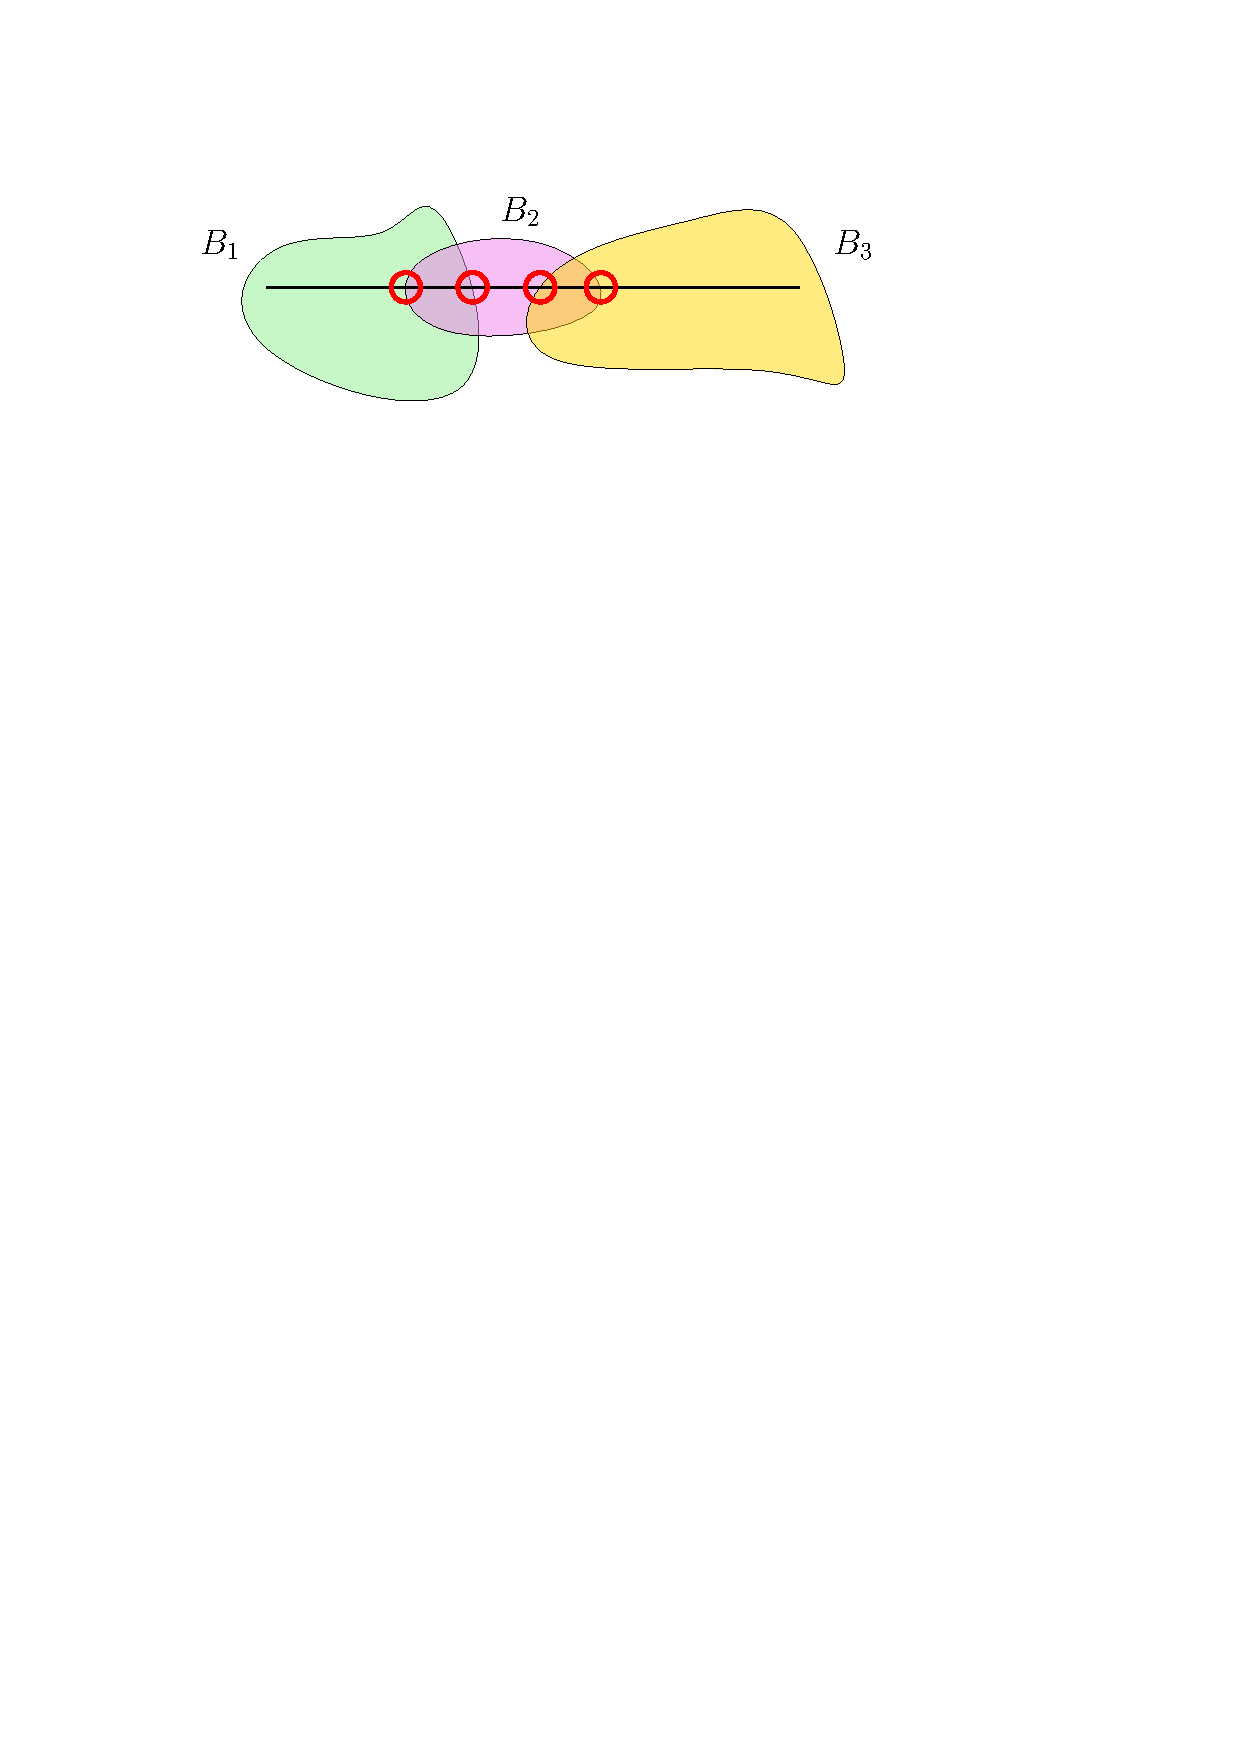
\includegraphics[scale=\normalipe]{ch01-usecka-pokryti-2.pdf}\\\qquad\\
    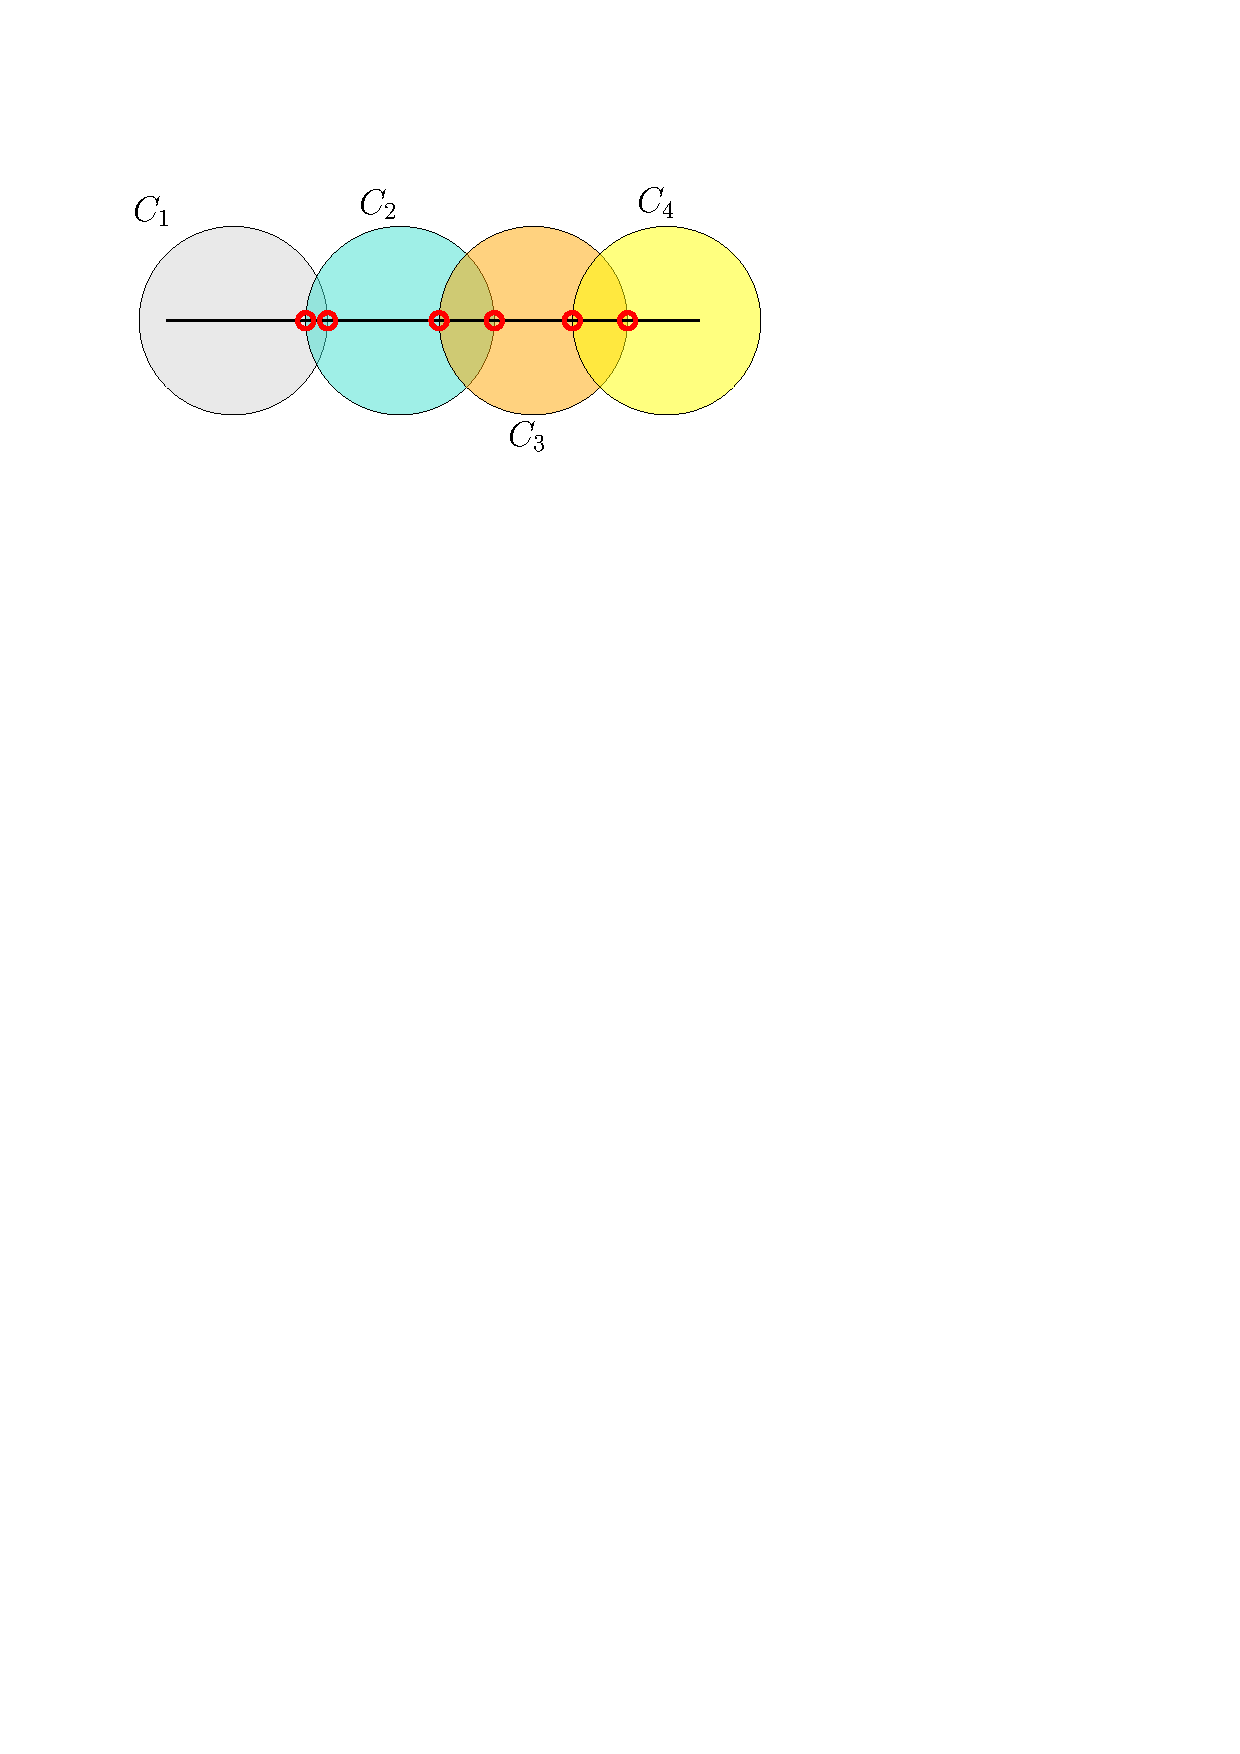
\includegraphics[scale=\normalipe]{ch01-usecka-pokryti-3.pdf}\\\qquad\\
    \caption{Různé možnosti (pod)pokrytí úsečky.}
    \label{fig:usecka-zjemneni}
\end{figure}
Pro libovolné pokrytí lze ukázat,~že každý bod je obsažen maximálně ve \emph{dvou množinách} vhodně zvoleného zjemnění,~tedy topologická dimenze úsečky je $1$. Podobně např. pro čtverec lze dojít k~závěru,~že pro každé pokrytí existuje zjemnění takové,~že každý bod obsažen maximálně ve \emph{třech množinách},~tedy jeho topologická dimenze je 2,~jak bychom očekávali (viz obrázek~\ref{fig:ctverec-zjemneni}).
\begin{figure}[h]
    \centering
    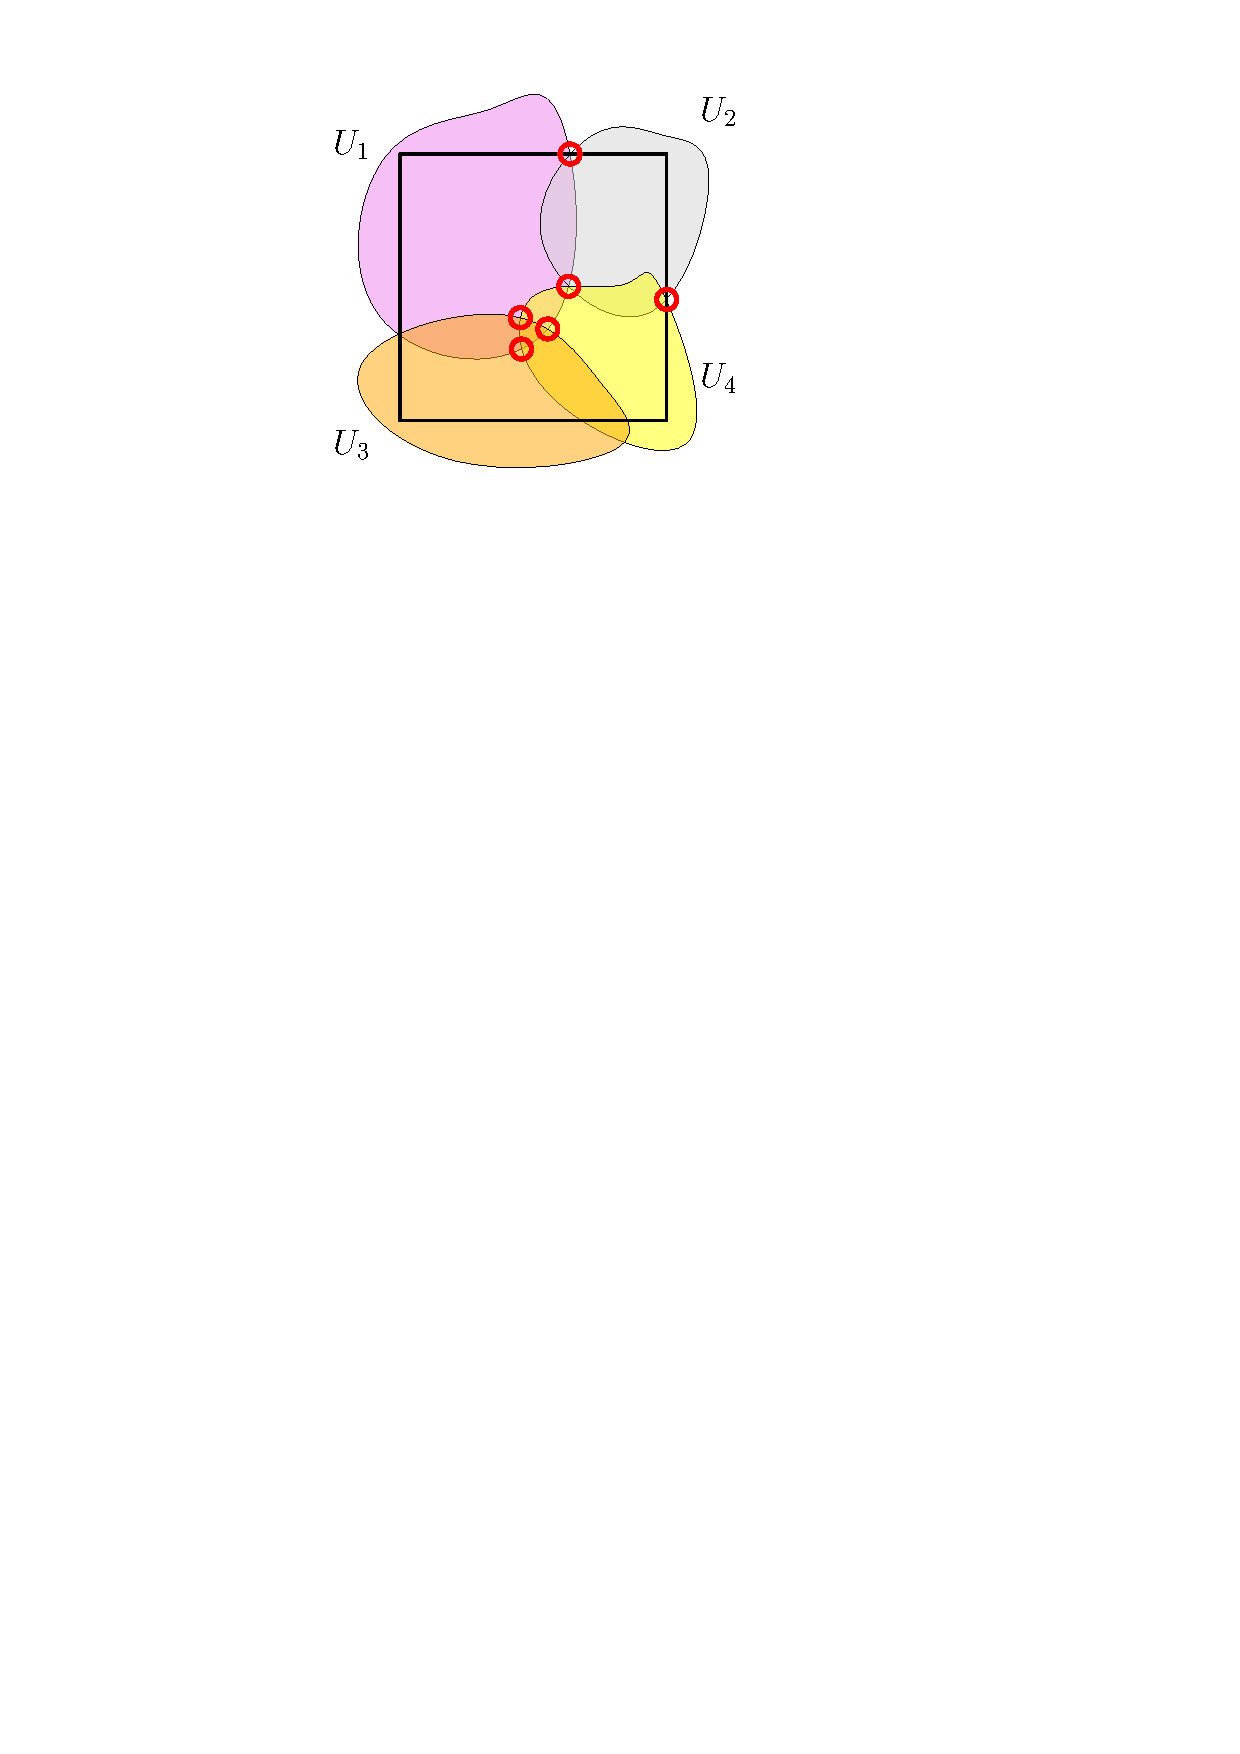
\includegraphics[scale=\normalipe]{ch01-ctverec-pokryti.pdf}
    \caption{Možné (pod)pokrytí čtverce.}
    \label{fig:ctverec-zjemneni}
\end{figure}
Porovnejme nyní topologickou dimenzi vůči dimenzi fraktální. Jak jsme se již přesvědčili v~příkladech~\ref{ex:fraktalni-dimenze-usecka},~\ref{ex:fraktalni-dimenze-ctverec} a~\ref{ex:fraktalni-dimenze-trojuhelnik},~pro "standardní" útvary je fraktální dimenze celočíselná (ač jsou i~další,~které jsme neuvedli),~zatímco v~podsekci~\ref{subsec:dimenze-fraktalu} jsme zjistili,~že u~fraktální dimenze fraktálů tomu tak být nemusí. Přitom však topologická dimenze fraktálních útvarů je (a dokonce musí být) celočíselná (viz tabulka~\ref{table:fraktalni-topologicka-dimenze}).
\begin{table}[h]
    \centering
    \begin{tabular}{r|cc}
    Útvar $F$                & $\dimB{F}$            & $\dimL{F}$ \\\hline
    Úsečka                   & 1                     & 1          \\
    Čtverec                  & 2                     & 2          \\
    Krychle                  & 3                     & 3          \\
    Teserakt                 & 4                     & 4          \\
    $d$-rozměrná krychle     & $d$                   & $d$        \\
    Kochova křivka           & $1{,}2618595\dots$    & 1          \\
    Kochova vločka           & $1{,}2618595\dots$    & 1          \\
    Sierpińského trojúhelník & $1{,}5849625\dots$    & 2          \\
    Cantorovo diskontinuum   & $0{,}6309297\dots$    & 0      
    \end{tabular}
    \caption{Porovnání fraktální a~topologické dimenze útvarů.}
    \label{table:fraktalni-topologicka-dimenze}
\end{table}
Fraktální dimenze tak oproti té topologické daleko lépe zachycuje informaci o~detailní geometrii daných objektů.
\section{Co je to fraktál?}\label{sec:co-je-to-fraktal}
\emph{Tak co je to tedy ten "fraktál"?}\index{fraktál} Odpovědi na tuto otázku jsme se poměrně dlouhou dobu vyhýbali a~onen termín,~popř. jeho přídavnou variantu \emph{"fraktální"},~jsme používali čistě na intuitivní úrovni. Ač jsme se zatím obešli bez jeho formálnějšího upřesnění,~bylo by možná při nejmenším slušné se o~to alespoň pokusit. V~předešlé sekci~\ref{sec:fraktalni_dimenze} jsme pokryli \emph{fraktální} a~\emph{topologickou dimenzi},~které jsme následně použili na příkladech konkrétních útvarů (konkrétně viz tabulky~\ref{table:fraktaly-eukleides-dimenze} a~\ref{table:fraktalni-topologicka-dimenze}).

Již jsme si všimli,~že u~fraktálních útvarů vychází fraktální dimenze $\dimH$ neceločíselně oproti jejich topologické dimenzi $\dimL$,~která je vždy celočíselná. To by se mohlo zdát jako dobrá charakteristika fraktálů. Avšak existují útvary,~jejichž fraktální a~topologická dimenze se shodují,~přestože také mají "fraktální charakter". Pro příklad nemusíme chodit nikterak daleko,~pravděpodobně nejznáměnším útvarem je v~tomto ohledu \emph{Mandelbrotova množina}\index{množina!Mandelbrotova}\index{Mandelbrotova mnozina},~jejiž fraktální i~topologická dimenze je rovna $2$ (blíže se na ni podíváme v~podsekci~\ref{subsec:mandebrotova-mnozina}). Jiná definice zase naopak popisuje fraktál jako útvar,~jehož Hausdorffova dimenze (na tu se blíže podíváme v~sekci~\ref{sec:hausdorffova-mira-dimenze}) je ostře větší než dimenze topologická. Problém (a také důvod,~proč jsme definici toho pojmu vyhývali) je však zkrátka ten,~že dodnes \textbf{není známá} žádná univerzální definice fraktálu. \cite[str. 226]{Voracova2022}

Je to možná lehce zklamávající,~nicméně dobrou zprávou je,~že ani pro další výklad ona absence formální definice fraktálu nebude překážkou. V~dalším textu se zaměříme (mj.) především na jejich klasifikaci (viz kapitola~\ref{chapter:klasifikace-fraktalu}) a~další vlastnosti.
\chapter{Teorie míry}\label{chapter:teorie-miry}
\todo{Doplnit kapitolu.}
\chapter{Klasifikace fraktálů}\label{chapter:klasifikace-fraktalu}
\todo{Doplnit text ke kapitole.}
\section{L-systémy}\label{sec:L-systemy}

Uvedeme tuto kapitolu s~ohledem na předchozí obsah trochu netradičně a od matematiky se (alespoň zdánlivě) na chvíli odkloníme. Podíváme se na fraktály,~s jejichž způsobem popisu přišel roku 1968 maďarský biolog \name{Aristid Lindenmayer} (1925--1989) a který (možná pro někoho i~překvapivě) má základy především v~informatice. \citep[str. 2]{Prusinkiewicz1990}

K popisu určitého fraktálů lze využít znalosti z \emph{teorie formálních jazyků} a \emph{teorie automatů}, na jejímž počátku stál (mj.) britský matematik a informatik \name{Alan Turing} (1912--1954). Ten ve svém článku \emph{On Computable Numbers, with an Application to the Entscheidungsproblem} z roku 1936 zavedl koncept abstraktního stroje dnes známého jako \emph{Turingův stroj}\index{Turingův stroj}, jednoduché zařízení s výpočetními schopnostmi již tehdy porovnatelnými se současnými počítači.
\begin{figure}[h]
    \centering
    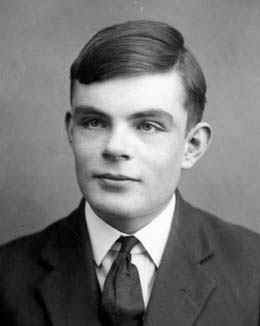
\includegraphics[width=.4\textwidth]{Alan-Turing.jpeg}
    \caption[Alan Turing,~1871--1956]{Alan Turing\footnote{Převzato z~\cite{OConnorTuring2025}},~1912--1954}
    \label{fig:alan-turing}
\end{figure}
V té době se zabýval otázkou, kterou v roce 1928 položil známý německý matematik \name{David Hilbert} (1862--1943), jež je známá pod názvem \emph{"Entscheidungsproblem"}\index{Entscheidungsproblem}\footnote{Anglicky \emph{The Decision problem}\index{The Decision problem}, česky přeložitelné jako \emph{"rozhodovací problém"}. Zde avšak poznamenejme, že onem český termín se používá i v související teorii složitosti a vyčíslitelnosti, má však podstatně jiný význam.}. Problémem bylo, zda existuje algoritmus, který o každém tvrzení je schopný rozhodnout (v konečném čase), zda je či není pravdivé. Později Alan Turing tento problém přeformuloval takto: \emph{Existuje program, který o jiném programu na vstupu rozhodne, zda se zastaví, či nikoliv?} David Hilbert byl ve svých vizích optimistický, avšak nakonec Alan Turing dokázal, že \textbf{takový algoritmus nemůže existovat}. Způsob, jakým Turing došel onomu výsledku, byl v konečném důsledku vlastně až překvapivě jednoduchý a existuje pro něj velké množství popularizačních materiálů\footnote{Pokud by se chtěl čtenář dozvědět více o této problematice a teorii s ní související, doporučuji např. knihu \cite{Motwani2003}}.
\begin{figure}[h]
    \centering
    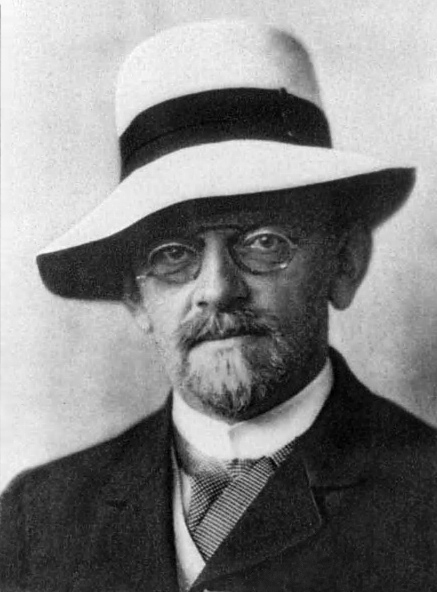
\includegraphics[width=.4\textwidth]{David-Hilbert.jpg}
    \caption[David Hilbert,~1871--1956]{David Hilbert\footnote{Převzato z~\cite{OConnorHilbert2025}},~1862--1943}
    \label{fig:david-hilbert}
\end{figure}
\section{Systém iterovaných funkcí}\label{sec:ifs}

V předchozí části kapitoly jsme viděli, jak lze fraktální objekty efektivně popisovat pomocí L-systémů, kde struktura vzniká paralelním přepisováním symbolů a~jejich vizualizace se provádí prostřednictvím želví grafiky. Tento přístup nám umožňoval popsat určitou skupinu fraktálů, nicméně pro jiné fraktály by se nám hodil vhodnější popis jejich konstrukce. Např. Sierpińského trojúhelník lze generovat pomocí L-systému, nicméně v~sekci~\ref{sec:sobepodobnost} o~soběpodobnosti jsme si jej záváděli spíše pomocí opakované aplikace určitých geometrických transformací (ač jsme neuvedli jejich explicitní vyjádření). Ty si později zavedeme jako tzv. \emph{systémy iterovaných funkcí}\index{systém iterovaných funkcí}.

Nejdříve se podíváme trochu více na matematickou podstatu. Hodně záležitostí jsme si již rozebrali v~kapitole~\ref{chapter:hausdorffuv-mp} o~Hausdorffově metrickém prostoru\index{Hausdorffův metrický prostor}\index{metrický prostor!Hausdorffův}, který zde bude hrát významnou roli. Pro související matematickou teorii, kterou zde dále budeme vykládat, doporučuji knihu \cite{Barnsley1993}.

\subsection{Kontrakce na Hausdorffově metrickém prostoru}\label{subsec:hausdorffuv-mp-kontrakce}

V minulých kapitolách jsme se často zaměřovali na lipschitzovská a~bilipschitzovská zobrazení. V~tomto případě nás budou speciálně zajímat tzv. \emph{kontrakce}\index{kontrakce}\index{zobrazení!kontraktivní}. Těmto termínům a~faktům s~nimi souvisejícími jsme se krátce věnovali v~podsekci~\ref{subsec:lipschitzovska-zobrazeni}.

Připomeňme, že lipschitzovskost rovnou implikuje spojitost zobrazení v~libovolném metrickém prostoru $(X,\varrho)$. Ještě než však začneme, podíváme se na alternativní definici Hausdorffovy metriky, která se nám dále bude hodit.
\begin{theorem}[Alternativní definice Hausdorffovy metriky]\label{thm:alternativni-hausdorffova-metrika}
    Nechť $(X,\varrho)$ je metrický prostor. Pro každé $A,B\in\hyperspace(X)$ platí
    \[\hausdorffmetric(A,B)=\max\set{\sup_{x\in A}\varrho(x,B),\sup_{y\in B}\varrho(y,A)}.\]
\end{theorem}
\begin{proof}
    Nechť je dáno $\varepsilon>0$ takové, že $\varepsilon\geqslant\hausdorffmetric(A,B)$. Pak $A\subseteq(B)_\varepsilon$ a~$B\subseteq(A)_\varepsilon$, tzn.
    \[\varepsilon\geqslant\max\set{\sup_{x\in A}\varrho(x,B),\sup_{y\in B}\varrho(y,A)}.\]
    Naopak zvolíme-li $0<\varepsilon\leqslant\hausdorffmetric(A,B)$, pak určitě platí alespoň jedna z~nerovností:
    \[\varepsilon\leqslant\sup_{x\in A}\varrho(x,B)\quad\text{nebo}\quad\varepsilon\leqslant\sup_{y\in B}\varrho(y,A).\]
    Tedy
    \[\varepsilon\leqslant\max\set{\sup_{x\in A}\varrho(x,B),\sup_{y\in B}\varrho(y,A)}.\]
    Z~toho dostáváme závěr tvrzení.
\end{proof}

Jako první se podíváme na trojici pomocných lemmat.
\begin{lemma}\label{lem:spojitost-a-hyperprostor}
    Nechť $\mapping{f}{X}{X}$ je spojisté zobrazení v~metrickém prostoru $(X,\varrho)$. Pak pro každé $S\in\hyperspace(X)$ platí $f(S)\in\hyperspace(X)$.
\end{lemma}
\begin{proof}
    Nechť $S\in\hyperspace(X)$. Zjevně platí $f(S)\neq\emptyset$. Pro důkaz kompaktnosti $f(S)$ uvažujme posloupnost $\set{x_n}_{n=1}^\infty$, kde $x_i\in S$ pro každé $i\in\N$. Protože $S$ je kompaktní, existuje posloupnost indexů $\set{n_k}_{k=1}^\infty$, taková, že $x_{n_k}\to x\in S$. Ze spojitosti zobrazení $f$ však plyne, že pak $\set{f(x_{n_k})}_{k=1}^\infty$ je podposloupností posloupnosti $\set{f(x_n)}_{n=1}^\infty$ a~$f(x_{n_k})\to f(x)$, tedy i~$f(S)$ je kompaktní.
\end{proof}
\begin{lemma}\label{lem:kontrakce-a-hyperprostor}
    Nechť $\mapping{f}{X}{X}$ je kontrakce na metrickém prostoru $(X,\varrho)$ s~faktorem $0<K<1$. Pak $\mapping{f}{\hyperspace(X)}{\hyperspace(X)}$ je kontrakce na Hausdorffově metrickém prostoru s~faktorem $K$.
\end{lemma}
(Převzato z~\citep[str. 79]{Barnsley1993}.)
\begin{proof}
    Z~předchozího lemmatu~\ref{lem:spojitost-a-hyperprostor} víme, že $f(S)\in\hyperspace(X)$ pro každé $S\in\hyperspace(X)$. Mějme množiny $A,B\in\hyperspace(X)$. Pak
    \begin{align*}
        \varrho(f(A),f(B))&=\inf\set{\varrho(f(x),f(y))\mid x\in A\;,\;y\in B}\\
        &\leqslant\inf\set{K\cdot\varrho(x,y)\mid x\in A\;,\;y\in B}\\
        &=K\cdot\inf\set{\varrho(x,y)\mid x\in A\;,\;y\in B}\\
        &=K\cdot\varrho(A,B).
    \end{align*}
    Tedy celkově
    \begin{align*}
        \hausdorffmetric(f(A),f(B))&=\inf\set{\delta>0\mid f(A)\subseteq(f(B))_\delta\land f(B)\subseteq(f(A))_\delta}\\
        &=\max\set{\sup_{x\in A}\varrho(f(x),f(B)),\sup_{y\in B}\varrho(f(y),f(A))}\\
        &=\max\set{\sup_{x\in A}\inf_{y\in B}\varrho(f(x),f(y)),\sup_{y\in B}\inf_{x\in A}\varrho(f(y),f(x))}\\
        &\leqslant K\max\set{\sup_{x\in A}\inf_{y\in B}\varrho(f(x),f(y)),\sup_{y\in B}\inf_{x\in A}\varrho(f(y),f(x))}\\
        &=K\hausdorffmetric(A,B).
    \end{align*}
    Druhá rovnost plyne z~věty~\ref{thm:alternativni-hausdorffova-metrika}.
\end{proof}
(Převzato a~upraveno z~\citep[str. 79]{Barnsley1993}.)
\begin{lemma}\label{lem:hausdorffova-metrika-odhad-sjednoceni}
    Pro každé množiny $A,B,C,D\in\hyperspace(X)$, kde $(X,\varrho)$ je metrický prostor, platí
    \[\hausdorffmetric(A\cup B,C\cup D)\leqslant\max\set{\hausdorffmetric(A,C),\hausdorffmetric(B,D)}.\]
\end{lemma}
\begin{proof}
    Budeme vycházet z~alternativní definice Hausdorffovy metriky, jejíž ekvivalenci s~původní definicí jsme dokázali výše (viz věta~\ref{thm:alternativni-hausdorffova-metrika}). Pro $\varrho(x,A\cup B)$ platí následující odhad:
    \[\varrho(x,A\cup B)=\min\set{\inf_{y\in A}\varrho(x,y),\inf_{z\in B}\varrho(x,z)}\leqslant\inf_{y\in A}\varrho(x,y)=\varrho(x,A).\]
    Z~toho pak máme
    \[\sup_{x\in A}\varrho(x,C\cup D)\leqslant\sup_{x\in A}\inf_{y\in C}\varrho(x,y)=\varrho(x,A)\leqslant\hausdorffmetric(A,C)\]
    a~tedy
    \[\sup_{x\in A\cup B}\varrho(x,C\cup D)\leqslant\max\set{\hausdorffmetric(A,C),\hausdorffmetric(B,D)}.\]
    Stejný odhad lze získat i~pro $\sup_{x\in C\cup D}\varrho(x,A\cup B)$:
    \begin{align*}
        \sup_{x\in C\cup D}\varrho(x,A\cup B)&=\max\set{\sup_{x\in C}\varrho(x,A\cup B),\sup_{x\in D}\varrho(x,A\cup B)}\\
        &\leqslant\max\set{\hausdorffmetric(C,A),\hausdorffmetric(D,B)}=\max\set{\hausdorffmetric(A,C),\hausdorffmetric(B,D)}.
    \end{align*}
    Tedy celkově lze psát
    \begin{align*}
        \hausdorffmetric(A\cup B,C\cup D)&=\max\set{\sup_{x\in A\cup B}\varrho(x,C\cup D),\sup_{x\in C\cup D}\varrho(x,A\cup B)}\\
        &\leqslant\max\set{\hausdorffmetric(A,C),\hausdorffmetric(B,D)}.
    \end{align*}
\end{proof}

Dvojice lemmat~\ref{lem:spojitost-a-hyperprostor} a~\ref{lem:kontrakce-a-hyperprostor} nám v~podstatě říká, že obrazem kompaktní množiny v~kontraktivním zobrazení\index{zobrazení!kontraktivní}\index{kontraktivní zobrazení} je opět kompaktní množina a~že "kontraktivita" zobrazení definovaného na libovolném metrickém prostoru $(X,\varrho)$ se zachovává na hyperprostoru. Tento výsledek se nám bude později hodit, neboť neboť jak již bylo zmíněno na začátku, některé fraktály lze konstruovat pomocí opakované aplikace určitých geometrických tranformací. Jak lze nejspíše z~dosavadního výkladu tušit, budeme pracovat právě s~kontrakcemi.
\begin{definition}[Systém iterovaných funkcí]\label{def:system-iterovanych-funkci}
    \emph{Systém iterovaných funkcí}\index{systém iterovaných funkcí}, zkráceně IFS (z anglického \emph{iterated function system}\index{iterated function system}), na metrickém prostoru $(X,\varrho)$ je konečná množina kontrakcí
    \[\set{\mapping{\psi_i}{X}{X}\mid 1\leqslant i\leqslant n}\]
    s~faktory $K_i$. Kontraktivním faktorem IFS je číslo $K=\max\set{K_i\mid 1\leqslant i\leqslant n}$.
\end{definition}
Zatím není zcela zjevné, proč definujeme pro IFS kontraktivní faktor jako maximum z~faktorů všech kontrakcí v~něm obsažených (byť to může působit do jisté míry intuitivně). Odpověď na tuto otázku nám poskytne následující věta~\ref{thm:sjednoceni-kontrakci}.
\begin{theorem}\label{thm:sjednoceni-kontrakci}
    Nechť $\set{\psi_1,\psi_2,\ldots,\psi_n}$ je IFS na metrickém prostoru $(X,\varrho)$ s~kontraktivním faktorem\index{faktor}\index{kontraktivní faktor}\index{faktor!kontraktivní} $0<K<1$. Pak zobrazení $\mapping{\Psi}{\hyperspace(X)}{\hyperspace(X)}$ definované předpisem
    \[\Psi(A)=\bigcup_{i=1}^n\psi_i(A)\]
    pro $A\in\hyperspace(X)$ je kontrakce na $(\hyperspace(X),\hausdorffmetric)$ s~faktorem $K$.
\end{theorem}
(Převzato z~\citep[str. 81]{Barnsley1993}.)
\begin{proof}
    Důkaz tvrzení lze provést indukcí podle $n$. V~případě, kdy $n=1$ je situace triviální. Pro $n=2$ zvolme množiny $A,B\in\hyperspace(X)$. Pak
    \begin{align*}
        \hausdorffmetric(\psi_1(A)\cup\psi_2(A),\psi_1(B)\cup\psi_2(B))&\leqslant\max\set{\hausdorffmetric(\psi_1(A),\psi_1(B)),\hausdorffmetric(\psi_2(A),\psi_2(B))}\\
        &\leqslant\max\set{K_1\hausdorffmetric(A,B),K_2\hausdorffmetric(A,B)}\\
        &\leqslant K\hausdorffmetric(A,B),
    \end{align*}
    kde druhá nerovnost plyne z~lemmatu~\ref{lem:hausdorffova-metrika-odhad-sjednoceni}. Nyní ukážeme, že zobrazení $\Psi
    $ definované předpisem $\Psi(A)=\bigcup_{i=1}^n\psi_i(A)$ je kontrakce. Mějme opět množiny $A,B\in\hyperspace(X)$. Pak
    \begin{align*}
        \hausdorffmetric(\Psi(A),\Psi(B))&=\hausdorffmetric\left(\left(\bigcup_{i=1}^{n-1}\psi_i(A)\right)\cup\psi_n(A),\left(\bigcup_{i=1}^{n-1}\psi_i(B)\right)\cup\psi_n(B)\right)\\
        &\leqslant\max\set{\hausdorffmetric\left(\bigcup_{i=1}^{n-1}\psi_i(A),\bigcup_{i=1}^{n-1}\psi_i(B)\right),\hausdorffmetric(\psi_n(A)\cup\psi_n(B))}\\
        &\stackrel{\text{I.P.}}{\leqslant}\max\set{K\hausdorffmetric(A,B),K_n\hausdorffmetric(A,B)}\leqslant K\hausdorffmetric(A,B).
    \end{align*}
\end{proof}
\begin{remark}
    Dodejme, že dále v~textu budeme používat značení $\Psi^{\circ n}$ definované induktivně:
    \begin{align*}
        \Psi^{\circ 0}&=\id,\\
        \Psi^{\circ n}&=\Psi\circ\Psi^{\circ(n-1)}\;,\;n\in\N.
    \end{align*}
    Tzn.~pro libovolnou množinu $B\in\hyperspace(X)$ je
    \[\Psi^{\circ 0}(B)=B\quad\text{a}\quad\Psi^{\circ n}(B)=\Psi(\Psi^{\circ(n-1)}(B)).\]
\end{remark}

S kontrakcemi se pojí známá věta z~matematické analýzy, která se nazývá \emph{Banachova věta o~pevném bodě} (viz~\ref{thm:banach}).
\begin{definition}[Pevný bod]\label{def:pevny-bod}
    Bod $x\in X$ se nazývá pevným bodem zobrazení $\mapping{f}{X}{X}$, pokud $f(x)=x$.
\end{definition}
\begin{theorem}[Banachova věta o~pevném bodě]\label{thm:banach}
    Nechť $(X,\varrho)$ je úplný metrický prostor a~zobrazení $\mapping{f}{X}{X}$ je kontrakce. Pak existuje právě jeden pevný bod $x\in X$ zobrazení $f$. Navíc volíme-li $x_0\in\N$ libovolně a~$x_n=f(x_{n-1})$ pro každé $n\in\N$, pak $x_n\to x$.
\end{theorem}
\begin{proof}
    Podle předpokladu je $f$ kontrakce s~faktorem $K$. Zvolme $x_0\in X$ a~dále pro každé $n\in\N$ položme $x_n=f(x_{n-1})$. Ukážeme, že takto definovaná posloupnost budů má limitu. Podle předpokladu je $(X,\varrho)$ úplný metrický prostor, tedy stačí ukázat, že posloupnost $\set{x_n}_{n=1}^\infty$ je cauchyovská. Pro vzdálenosti dvou po sobě jdoucích členů platí
    \begin{align*}
        \varrho(x_1,x_2)&=\varrho(f(x_0),f(x_1))\leqslant K\varrho(x_0,x_1),\\
        \varrho(x_2,x_3)&=\varrho(f(x_1),f(x_2))\leqslant K\varrho(x_1,x_2)\leqslant K^2\varrho(x_0,x_1),\\
        \varrho(x_3,x_4)&=\varrho(f(x_2),f(x_3))\leqslant K\varrho(x_2,x_3)\leqslant K^3\varrho(x_0,x_1),\\
        &\vdots\\
        \varrho(x_i,x_{i+1})&=\varrho(f(x_{i-1}),f(x_i))\leqslant K\varrho(x_{i-1},x_i)\leqslant K^i\varrho(x_0,x_1).\\
        &\vdots
    \end{align*}
    Pro odhadnutí vzdálenosti dvojice členů, které nejdou nutně bezprostředně po sobě použijeme trojúhelníkovou nerovnost. Volme $n,m\in\N$, pričemž $m>n$. Pak lze psát
    \begin{align*}
        \varrho(x_n,x_m)&\leqslant\sum_{i=n}^{m-1}\varrho(x_i,x_{i+1})\leqslant\sum_{i=n}^{m-1}K^i\varrho(x_0,x_1)=K^n\varrho(x_0,x_1)\sum_{i=1}^{m-n-1}K^i\\
        &=K^n\varrho(x_0,x_1)\cdot\dfrac{1-K^{n-m}}{K-1}.
    \end{align*}
    Výraz na pravé straně má pro $n\to\infty$ limitu $0$, tedy posloupnost $\set{x_n}_{n=1}^\infty$ je cauchyovská a~má limitu $x\in X$. Dále ze spojitosti funkce $f$ (neboť je lipschitzovská) plyne
    \[x=\lim_{n\to\infty}x_{n+1}=\lim_{n\to\infty}f(x_n)=f(x),\]
    tedy $x\in X$ je pevným bodem $f$. Jednoznačnost pevného bodu $x$ lze ukázat sporem. Pokud by existoval další pevný bod $y\neq x$, pak
    \[\varrho(x,y)=\varrho(f(x),f(y))\leqslant K\varrho(x,y).\]
    Protože $\varrho(x,y)>0$, musí být $K\geqslant 1$, což je spor s~předpokladem, že $f$ je kontrakce.
\end{proof}
Speciálně pro zobrazení $\Psi$ definované ve větě~\ref{thm:sjednoceni-kontrakci} nám Banachova věta~\ref{thm:banach} nejen říká, že má právě jeden pevný bod $A\in\hyperspace(X)$, tzn. $\Psi(A)=A$, ale zároveň udává způsob, jak daný pevný bod nalézt. Stačí opakovaně iterovat dané zobrazení.
\begin{definition}[Atraktor]\label{def:atraktor}
    Pevný bod $A\in\hyperspace(X)$ zobrazení $\Psi$ definovaného ve větě~\ref{thm:sjednoceni-kontrakci} pro libovolné IFS se nazývá \emph{atraktor}\index{atraktor}.
\end{definition}
Z Banachovy věty speciálně plyne, že atraktor $A$ libovolného IFS lze určit jako následující limitu:
\[A=\lim_{n\to\infty}\Psi^{\circ n}(B),\]
kde $B\in\hyperspace(X)$. Zajímavostí je fakt, že výsledný atraktor $A$ je zcela nezávislý na volbě množiny $B$. Tento fakt si ještě přiblížíme v~podsekci~\ref{subsec:fraktaly-ifs}.

V dalším textu budeme pracovat především s~afinními zobrazeními v~$\R^n$ se standardní eukleidovskou metrikou. Připomeňme si zde, že afinním zobrazením rozumíme jakékoliv zobrazení $\mapping{f}{X}{X}$, takové, že
\[f(x)=\mat{A}x+b,\]
kde $b\in X$ a~$\mat{A}$ je regulární matice. O~afinnitách lze též dokázat řadu zajímavých tvrzení, avšak tyto záležitosti již spadají spíše do oblasti lineární algebry. Nicméně v~případě každé z~afinnit, které zde dále uvidíme, se čtenář může celkem snadno přesvědčit, že se skutečně jedná o~kontrakci.

\subsection{Frakrály generované pomocí IFS}\label{subsec:fraktaly-ifs}

V předešlé podsekci~\ref{subsec:hausdorffuv-mp-kontrakce} jsme se společně podívali na některé důležité poznatky týkající se kontrakcí a~Hausdorffova metrického prostoru (viz kapitola~\ref{chapter:hausdorffuv-mp}). Na některá dokázaná tvrzení se zde budeme odkazovat.

Protože pracujeme s~fraktálními útvary v~rovině, tj. $\R^2$, afinní zobrazení, s nimiž budeme pracovat, budou mít tvar
\begin{equation}\label{eq:afinita-v-R2}
    \psi\left(\begin{matrix}
        x\\
        y
    \end{matrix}\right)=\underbrace{\left(\begin{matrix}
        a~& b\\
        c & d
    \end{matrix}\right)}_{\mat{A}}\left(\begin{matrix}
        x\\
        y
    \end{matrix}\right)+\left(\begin{matrix}
        e\\
        f
    \end{matrix}\right).
\end{equation}
Připomeňme, že matice $\mat{A}$ je regulární. Podíváme se na některé fraktály, které jsme již viděli v~úvodní kapitole~\ref{chapter:uvod_do_fraktalu} v~sekci~\ref{sec:sobepodobnost}. Jiný způsob generování těchto a~mnohých jiných fraktálních útvarů nám poskytují L-systémy, které jsme si ilustrovali v~sekci~\ref{sec:L-systemy}.

Znovu se podívejme na asi jeden z~nejznáměnších fraktálů z~této kategorie -- Sierpińského trojúhelník. Jeho konstrukce lze docílit pomocí IFS $\set{\omega_1,\omega_2,\omega_3}$, přičemž $\mapping{\omega_1,\omega_2,\omega_3}{\R^2}{\R^2}$ a~jednotlivé kontrakce jsou definovány následujícími předpisy:
\begin{align*}
    \omega_1\left(\begin{matrix}
        x\\
        y
    \end{matrix}\right)&=\left(\begin{matrix}
        1/2 & 0\\
        0 & 1/2
    \end{matrix}\right)\left(\begin{matrix}
        x\\
        y
    \end{matrix}\right)+\left(\begin{matrix}
        0\\
        0
    \end{matrix}\right),\\
    \omega_2\left(\begin{matrix}
        x\\
        y
    \end{matrix}\right)&=\left(\begin{matrix}
        1/2 & 0\\
        0 & 1/2
    \end{matrix}\right)\left(\begin{matrix}
        x\\
        y
    \end{matrix}\right)+\left(\begin{matrix}
        1/2\\
        0
    \end{matrix}\right),\\
    \omega_3\left(\begin{matrix}
        x\\
        y
    \end{matrix}\right)&=\left(\begin{matrix}
        1/2 & 0\\
        0 & 1/2
    \end{matrix}\right)\left(\begin{matrix}
        x\\
        y
    \end{matrix}\right)+\left(\begin{matrix}
        1/4\\
        \sqrt{3}/4
    \end{matrix}\right).
\end{align*}
Tedy zobrazení $\mapping{\Omega}{\hyperspace(\R^2)}{\hyperspace(\R^2)}$ definujeme jako
\[\Omega(A)=\omega_1(A)\cup\omega_2(A)\cup\omega_3(A),\]
kde $A\in\hyperspace(\R^2)$. Připomeňme, že takto definované $\Omega$ je (podle věty~\ref{thm:sjednoceni-kontrakci}) kontrakce a~tedy z~Banachovy věty o~pevném bodě plyne (viz věta~\ref{thm:banach}), že má právě jeden atraktor, tj. množinu $A\in\hyperspace(\R^2)$ takovou, že platí $A=\Omega(A)$. Kontraktivní faktor tohoto (ani jiného) IFS nás vyloženě zajímat nemusí, avšak není těžké jej dopočítat. Např. zde je celkem zjevné, že $K=1/2$. Užitečnější je však pro nás fakt, že atraktor $A$ lze určit jako
\[A=\lim_{n\to\infty}\Omega^{\circ n}(B),\]
kde $B\in\hyperspace(\R^2)$. V~našem případě je počátečním útvarem rovnostranný trojúhelník $T$, jehož vrcholy mají souřadnice
\[\left(\begin{matrix}
    0\\
    0
\end{matrix}\right),\;\left(\begin{matrix}
    1\\
    0
\end{matrix}\right),\;\left(\begin{matrix}
    1/2\\
    \sqrt{3}/2
\end{matrix}\right).\]
Prvních několik iterací zobrazení $\Omega$ si lze prohlédnout na obrázku~\ref{fig:iterace-zobrazeni-omega-sierpinskeho-trojuhelnik}. Sierpińského trojúhelník je tedy atraktorem zobrazení $\Omega$.

Zajímavostí je, že atraktor daného IFS je zcela nezávislý na volbě počátečního útvaru. Ač je tedy běžné, že v~případě Sierpińského trojúhelníka začínáme s~rovnostranným trojúhelníkem, faktem je, že je zcela lhostejné\footnote{Z formálního hlediska je třeba, aby se jednalo o~kompaktní neprázdnou množinu, nicméně v~$\R^n$ stačí pro tento účel uvažovat všechny neprázdné množiny, které jsou \emph{uzavřené a~omezené} (viz věta~\ref{thm:heine-borel})}, s jakým útvarem začneme (viz obrázek~\ref{fig:iterace-zobrazeni-omega-sierpinskeho-trojuhelnik-jiny-poc-utvar}).

Vypisovat explicitně dané kontrakce je sice formálně žádoucí, nicméně dosti nepraktické. Dále tedy budeme hodnoty jednotlivých koeficientů $a,b,\ldots,f$ (viz \eqref{eq:afinita-v-R2}) zapisovat do tabulky.
\begin{table}[h]
    \centering
    \begin{tabular}{c|cccccc}
    Kontrakce  & $a$   & $b$ & $c$ & $d$   & $e$   & $f$          \\\hline
    $\omega_1$ & $1/2$ & $0$ & $0$ & $1/2$ & $0$   & $0$          \\
    $\omega_2$ & $1/2$ & $0$ & $0$ & $1/2$ & $1$   & $0$          \\
    $\omega_3$ & $1/2$ & $0$ & $0$ & $1/2$ & $1/4$ & $\sqrt{3}/2$ \\
    \end{tabular}
    \caption{Koeficienty IFS $\Omega$ pro Sierpińského trojúhelník}
    \label{table:ifs-sierpinskeho-trojuhelnik}
\end{table}
U Wacłava Sierpińského se ještě chvíli zdržíme, neboť princip konstrukce jeho pravděpodobně nejznámenšího fraktálu lze přenést i~na další útvary. Jiným takovým příkladem je tzv. \emph{Sierpińského koberec}\index{Sierpińského koberec} jehož IFS si označíme $\Phi$ (viz tabulka~\ref{table:ifs-sierpinskeho-koberec}). I~v tomto případě (podobně jako u~Sierpińského trojúhelníka) lze začít s~libovolným útvarem. 
\begin{table}[h]
    \centering
    \begin{tabular}{c|cccccc}
    Kontrakce  & $a$   & $b$ & $c$ & $d$   & $e$   & $f$          \\\hline
    $\varphi_1$ & $1/3$ & $0$ & $0$ & $1/3$ & $0$   & $0$         \\
    $\varphi_2$ & $1/3$ & $0$ & $0$ & $1/3$ & $0$   & $1/3$         \\
    $\varphi_3$ & $1/3$ & $0$ & $0$ & $1/3$ & $0$   & $2/3$         \\
    $\varphi_4$ & $1/3$ & $0$ & $0$ & $1/3$ & $1/3$   & $2/3$         \\
    $\varphi_5$ & $1/3$ & $0$ & $0$ & $1/3$ & $1/3$   & $0$         \\
    $\varphi_6$ & $1/3$ & $0$ & $0$ & $1/3$ & $2/3$   & $0$         \\
    $\varphi_7$ & $1/3$ & $0$ & $0$ & $1/3$ & $2/3$   & $0$         \\
    $\varphi_8$ & $1/3$ & $0$ & $0$ & $1/3$ & $2/3$   & $0$
    \end{tabular}
    \caption{Koeficienty IFS $\Phi$ pro Sierpińského koberec}
    \label{table:ifs-sierpinskeho-koberec}
\end{table}
Pro ukázku viz obrázek~\ref{fig:iterace-zobrazeni-fi-sierpinskeho-koberec}.
\clearpage
\begin{figure}[h]
    \centering
    \begin{subfigure}{0.45\textwidth}
        \centering
        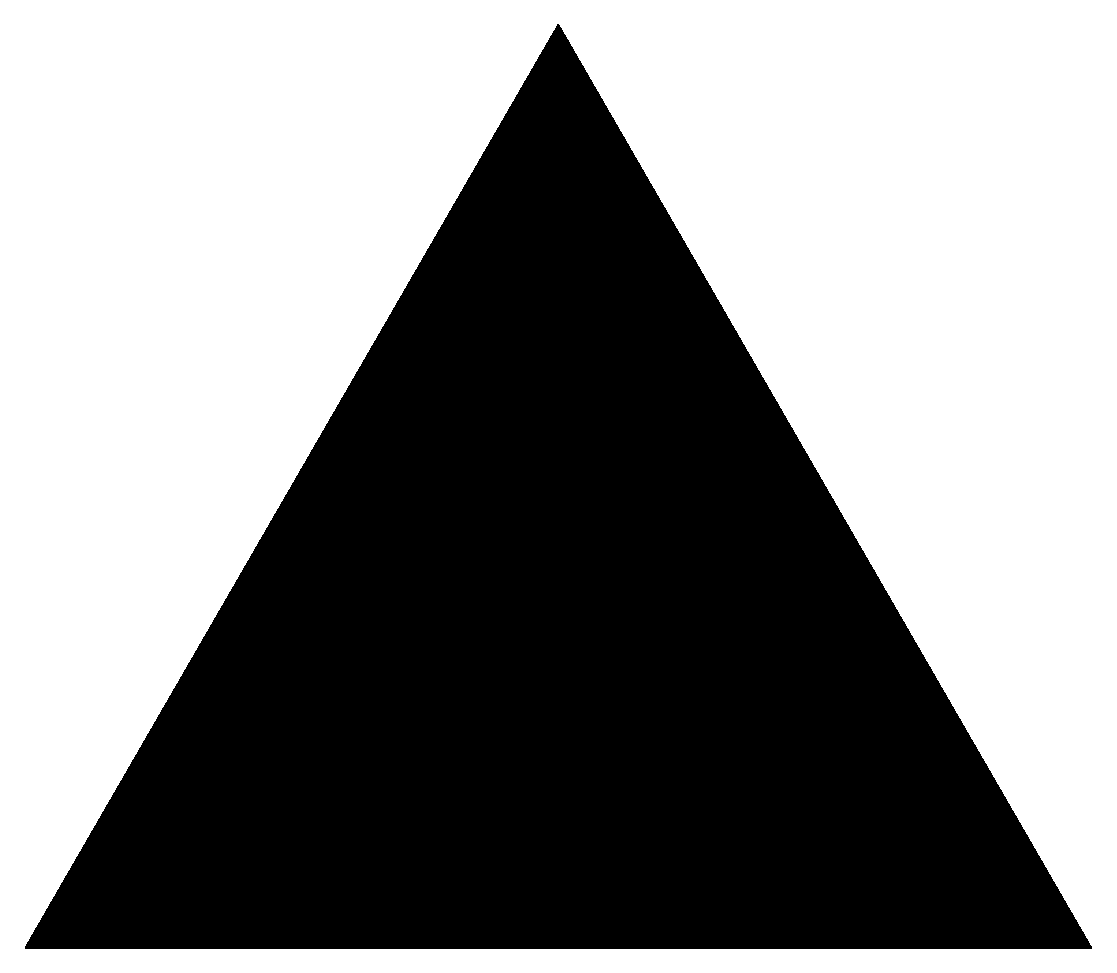
\includegraphics[width=\textwidth]{sierpinsky-triangle-iter0.pdf}
        \begin{center}
            $n=0$
        \end{center}
    \end{subfigure}
    \qquad
    \vspace{1cm}
    \begin{subfigure}{0.45\textwidth}
        \centering
        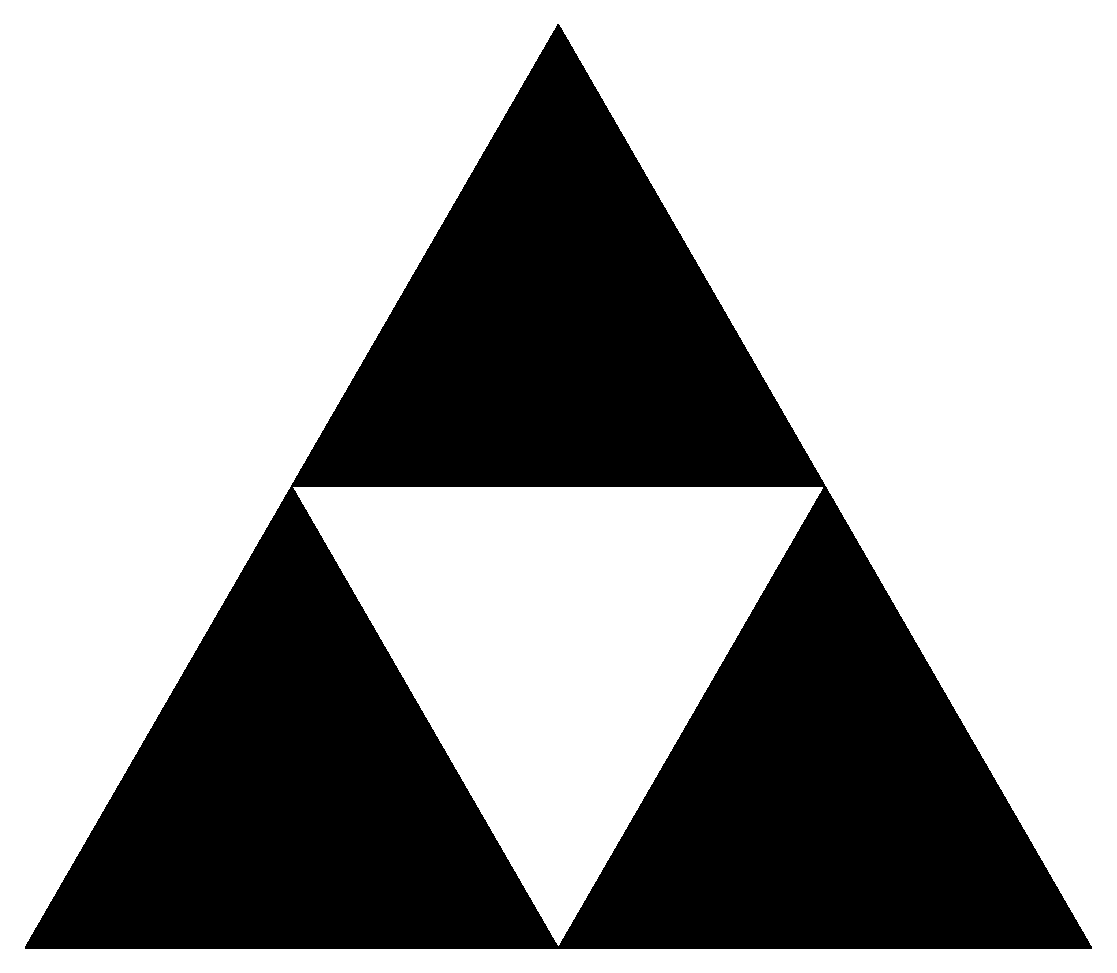
\includegraphics[width=\textwidth]{sierpinsky-triangle-iter1.pdf}
        \begin{center}
            $n=1$
        \end{center}
    \end{subfigure}
    \qquad
    \begin{subfigure}{0.45\textwidth}
        \centering
        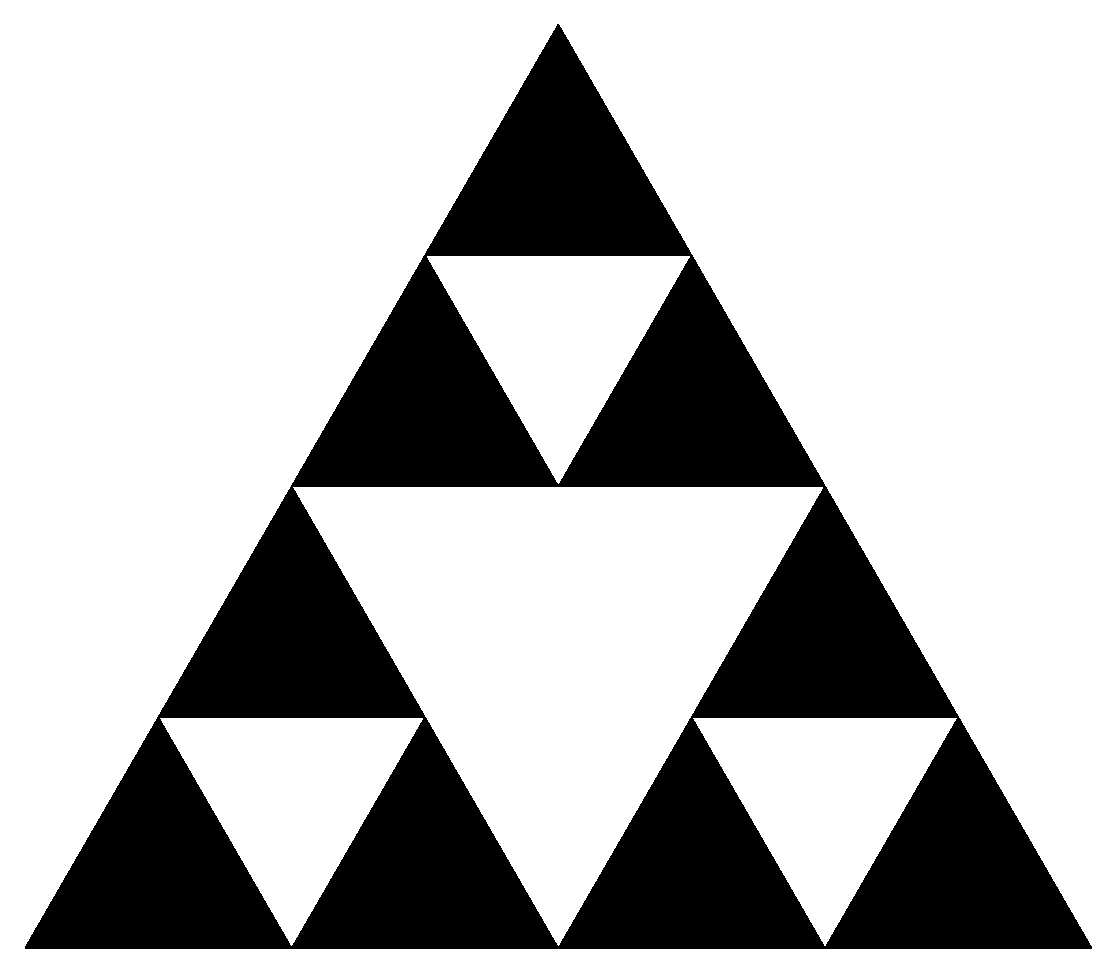
\includegraphics[width=\textwidth]{sierpinsky-triangle-iter2.pdf}
        \begin{center}
            $n=2$
        \end{center}
    \end{subfigure}
    \qquad
    \vspace{1cm}
    \begin{subfigure}{0.45\textwidth}
        \centering
        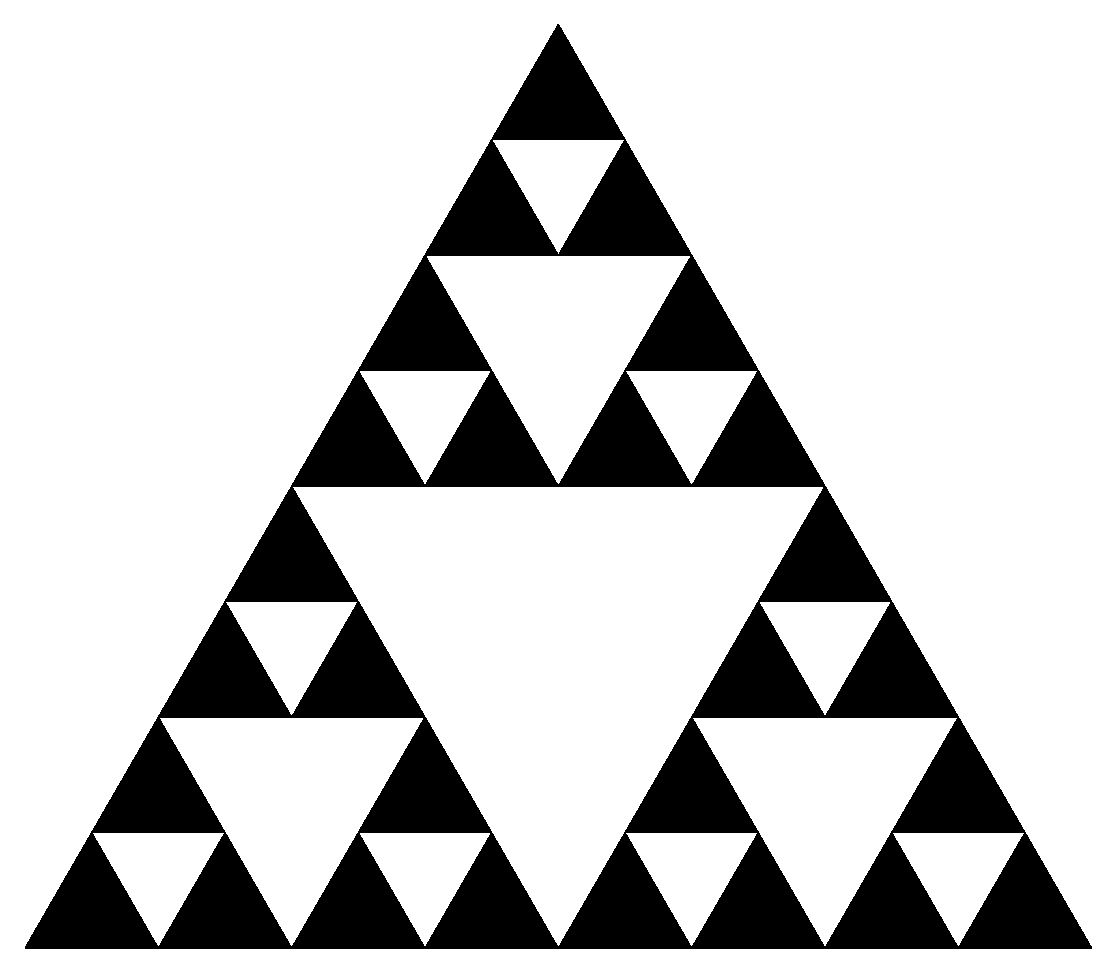
\includegraphics[width=\textwidth]{sierpinsky-triangle-iter3.pdf}
        \begin{center}
            $n=3$
        \end{center}
    \end{subfigure}
    \qquad
    \begin{subfigure}{0.45\textwidth}
        \centering
        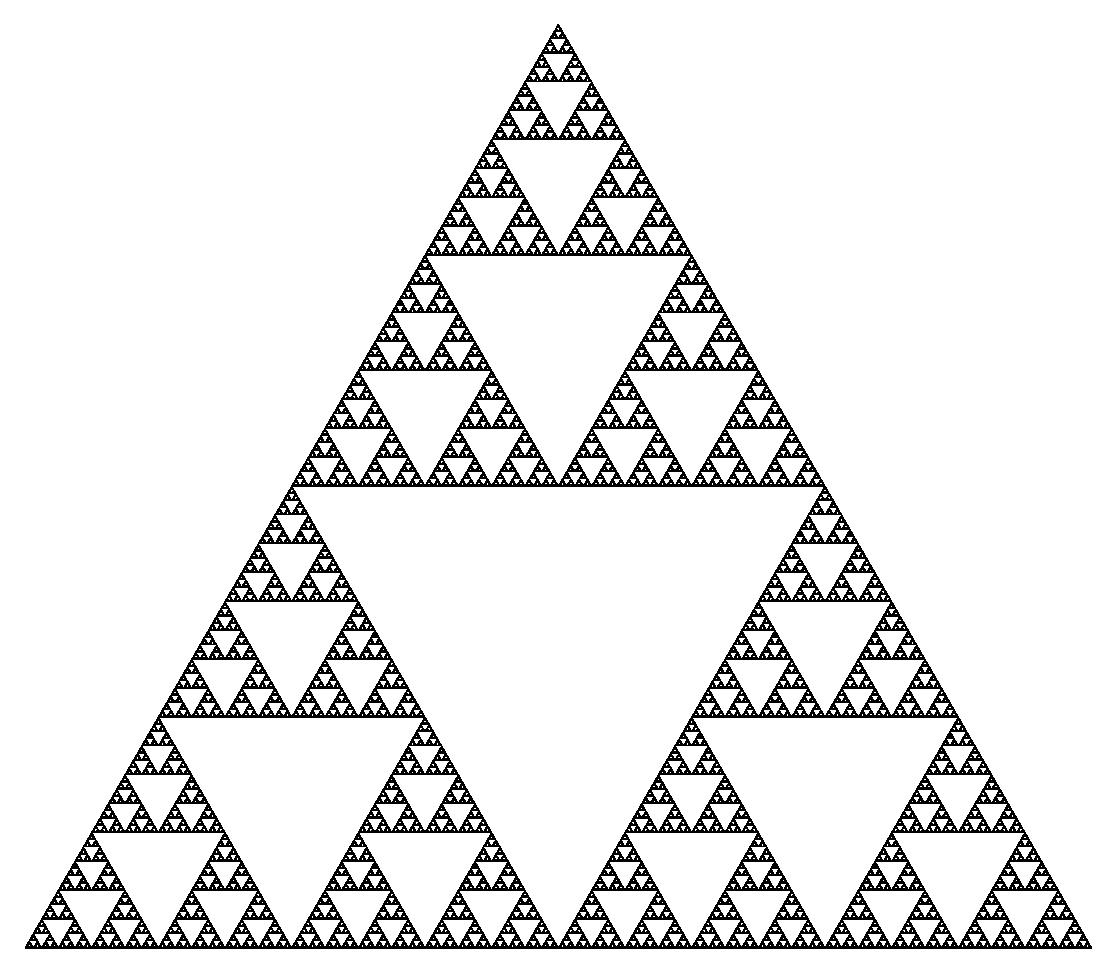
\includegraphics[width=\textwidth]{sierpinsky-triangle-iter8.pdf}
        \begin{center}
            $n=8$
        \end{center}
    \end{subfigure}
    \caption{Iterace zobrazení $\Omega$  (Sierpińského trojúhelník)}
    \label{fig:iterace-zobrazeni-omega-sierpinskeho-trojuhelnik}
\end{figure}
\clearpage
\begin{figure}[H]
    \centering
    \begin{subfigure}{0.45\textwidth}
        \centering
        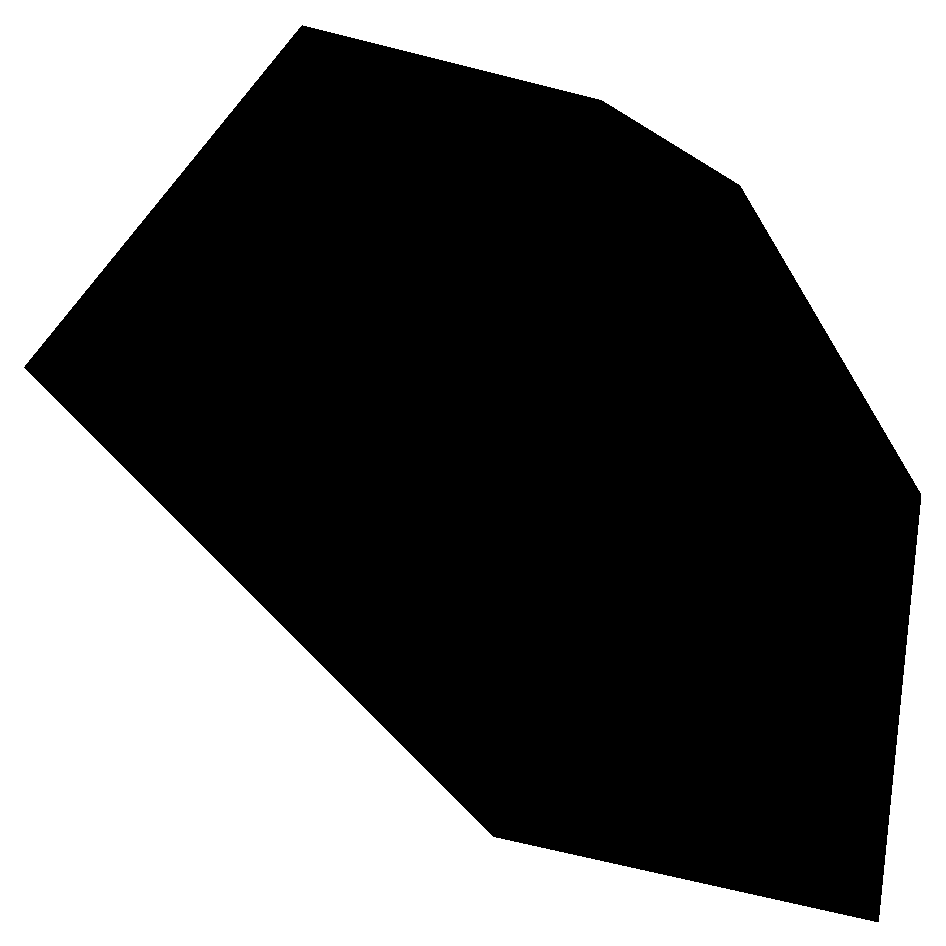
\includegraphics[width=\textwidth]{sierpinsky-triangle-2-iter0.pdf}
        \begin{center}
            $n=0$
        \end{center}
    \end{subfigure}
    \qquad
    \vspace{1cm}
    \begin{subfigure}{0.45\textwidth}
        \centering
        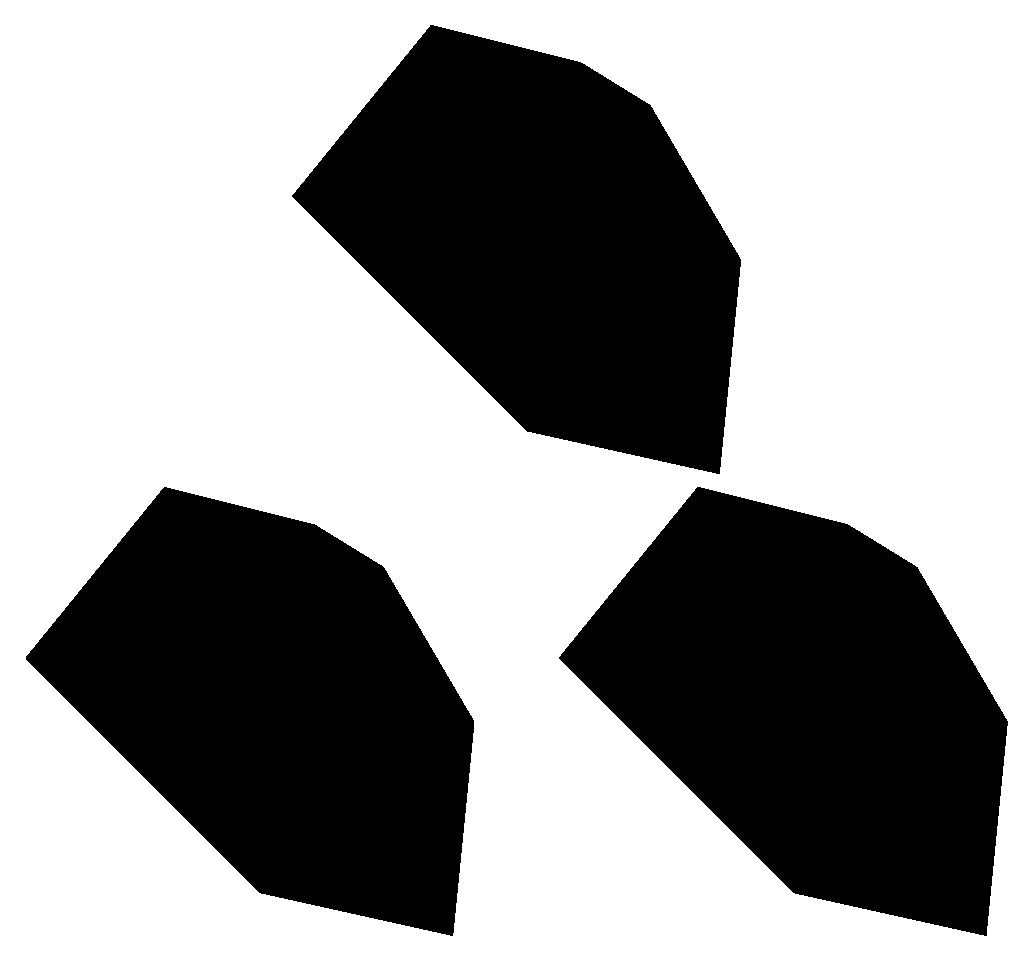
\includegraphics[width=\textwidth]{sierpinsky-triangle-2-iter1.pdf}
        \begin{center}
            $n=1$
        \end{center}
    \end{subfigure}
    \qquad
    \begin{subfigure}{0.45\textwidth}
        \centering
        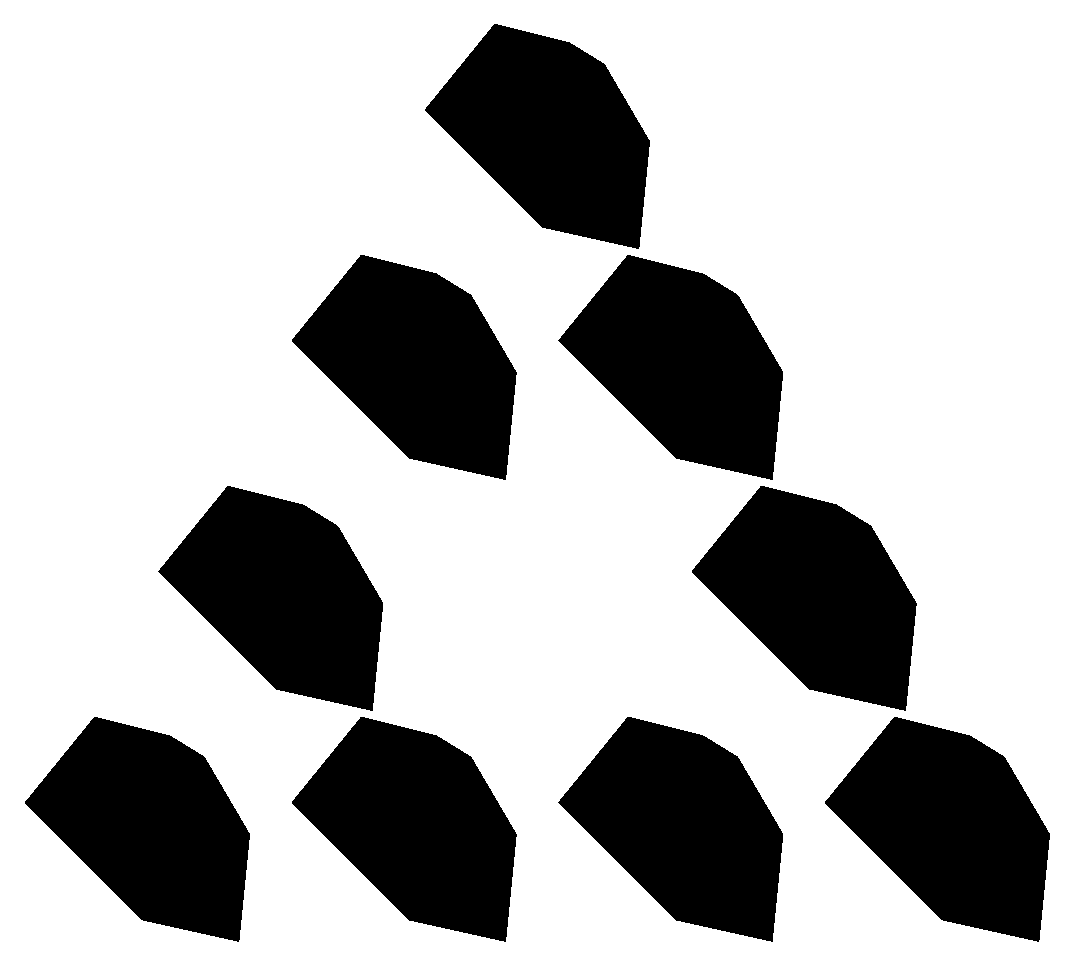
\includegraphics[width=\textwidth]{sierpinsky-triangle-2-iter2.pdf}
        \begin{center}
            $n=2$
        \end{center}
    \end{subfigure}
    \qquad
    \vspace{1cm}
    \begin{subfigure}{0.45\textwidth}
        \centering
        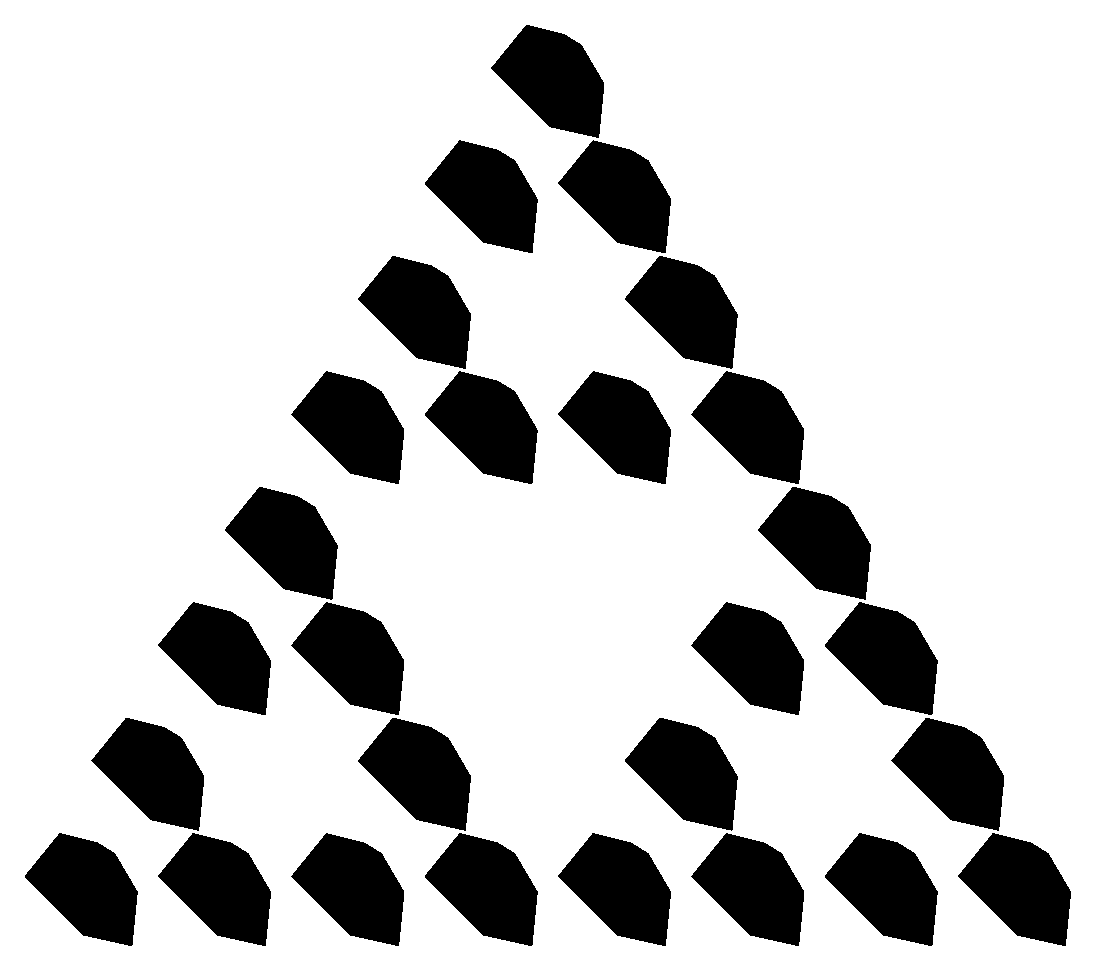
\includegraphics[width=\textwidth]{sierpinsky-triangle-2-iter3.pdf}
        \begin{center}
            $n=3$
        \end{center}
    \end{subfigure}
    \qquad
    \begin{subfigure}{0.45\textwidth}
        \centering
        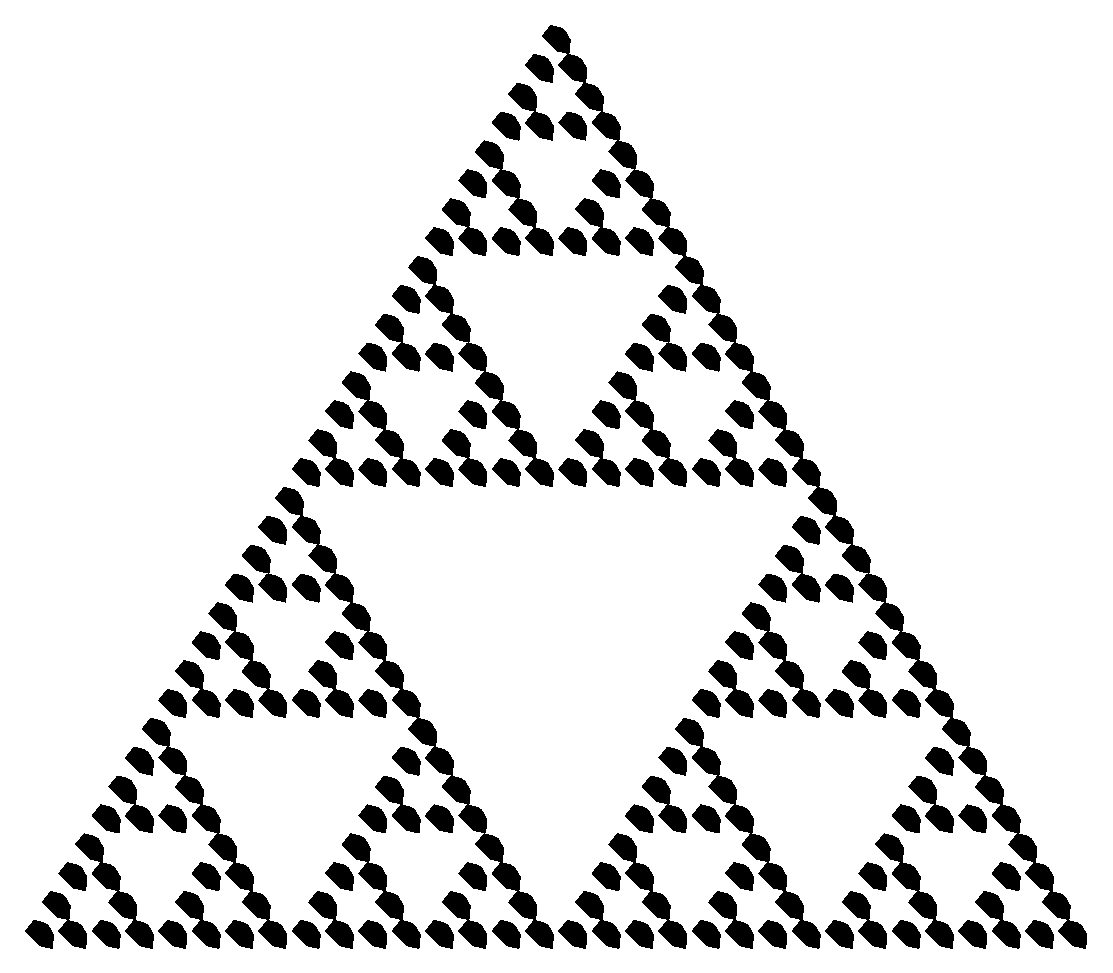
\includegraphics[width=\textwidth]{sierpinsky-triangle-2-iter5.pdf}
        \begin{center}
            $n=5$
        \end{center}
    \end{subfigure}
    \qquad
    \begin{subfigure}{0.45\textwidth}
        \centering
        \includegraphics[width=\textwidth]{sierpinsky-triangle-2-iter8.pdf}
        \begin{center}
            $n=8$
        \end{center}
    \end{subfigure}
    \caption{Iterace zobrazení $\Omega$ s~jiným počátečním útvarem $B$}
    \label{fig:iterace-zobrazeni-omega-sierpinskeho-trojuhelnik-jiny-poc-utvar}
\end{figure}
\begin{figure}[H]
    \centering
    \begin{subfigure}{0.45\textwidth}
        \centering
        \includegraphics[width=\textwidth]{sierpinsky-carpet-iter0.pdf}
        \begin{center}
            $n=0$
        \end{center}
    \end{subfigure}
    \qquad
    \vspace{1cm}
    \begin{subfigure}{0.45\textwidth}
        \centering
        \includegraphics[width=\textwidth]{sierpinsky-carpet-iter1.pdf}
        \begin{center}
            $n=1$
        \end{center}
    \end{subfigure}
    \qquad
    \begin{subfigure}{0.45\textwidth}
        \centering
        \includegraphics[width=\textwidth]{sierpinsky-carpet-iter2.pdf}
        \begin{center}
            $n=2$
        \end{center}
    \end{subfigure}
    \qquad
    \vspace{1cm}
    \begin{subfigure}{0.45\textwidth}
        \centering
        \includegraphics[width=\textwidth]{sierpinsky-carpet-iter3.pdf}
        \begin{center}
            $n=3$
        \end{center}
    \end{subfigure}
    \qquad
    \begin{subfigure}{0.45\textwidth}
        \centering
        \includegraphics[width=\textwidth]{sierpinsky-carpet-iter5.pdf}
        \begin{center}
            $n=5$
        \end{center}
    \end{subfigure}
    \caption{Iterace zobrazení $\Phi$ (Sierpińského koberec)}
    \label{fig:iterace-zobrazeni-fi-sierpinskeho-koberec}
\end{figure}

\subsection{Další fraktály a~jejich IFS}\label{subsec:fraktaly-a-jejich-ifs}

V této podsekci se podíváme na některé další příklady fraktálů a~jejich IFS. I~zde jsou všechny obrázky vygenerovány pomocí přiloženého programu\footnote{viz odkaz na GitHub repozitář: \url{https://github.com/D4vEOFF/Py-Fractal-Generator}}.
\begin{figure}[H]
    \centering
    \includegraphics[width=0.8\textwidth]{pythagorean-tree-iter10.pdf}
    \begin{center}
        $n=10$
    \end{center}
    \begin{tabular}{c|cccccc}
    Zobrazení   & $a$   & $b$   & $c$   & $d$   & $e$   & $f$          \\\hline
    $\psi_1$    & $1/2$ & $-1/2$ & $1/2$ & $1/2$ & $0$   & $1$         \\
    $\psi_2$    & $1/2$ & $1/2$ & $-1/2$ & $1/2$ & $1/2$ & $3/2$         \\
    $\psi_3$    & $1$   & $0$   & $0$   & $1$   & $0$   & $0$         \\
    \end{tabular}
    \caption{Pythágorův strom}
    \label{fig:pythagoruv-strom}
\end{figure}
Zde upozorněme však na fakt, že u~Pythágorova stromu na obrázku~\ref{fig:pythagoruv-strom} zobrazení $\psi_3$ je identita, která není kontrakcí, čili na takový systém nelze aplikovat větu~\ref{thm:sjednoceni-kontrakci}. Toto zobrazení je zde však čistě z~estetických důvodů, aby původní obrazec nezměnil svoji pozici v~další iteraci. Systém $\set{\psi_1,\psi_2}$ již představuje IFS s~jednoznačným atraktorem.
\begin{figure}[H]
    \centering
    \includegraphics[width=0.8\textwidth]{levi-dragon-iter12.pdf}
    \begin{center}
        $n=12$
    \end{center}
    \begin{tabular}{c|cccccc}
    Kontrakce   & $a$   & $b$   & $c$   & $d$   & $e$   & $f$          \\\hline
    $\psi_1$    & $1/2$ & $-1/2$ & $1/2$ & $1/2$ & $0$   & $0$         \\
    $\psi_2$    & $1/2$ & $1/2$ & $-1/2$ & $1/2$ & $1/2$ & $1/2$
    \end{tabular}
    \caption{Lévyho drak}
    \label{fig:levyho-drak}
\end{figure}
\begin{figure}[H]
    \centering
    \includegraphics[width=0.8\textwidth]{heighway-dragon-iter15.pdf}
    \begin{center}
        $n=15$
    \end{center}
    \begin{tabular}{c|cccccc}
    Kontrakce   & $a$   & $b$   & $c$   & $d$   & $e$   & $f$          \\\hline
    $\psi_1$    & $1/2$ & $-1/2$ & $1/2$ & $1/2$ & $0$   & $0$         \\
    $\psi_2$    & $-1/2$ & $-1/2$ & $1/2$ & $-1/2$ & $1$ & $0$
    \end{tabular}
    \caption{Dračí křivka}
    \label{fig:draci-krivka}
\end{figure}
\begin{figure}[H]
    \centering
    \includegraphics[width=0.8\textwidth]{sierpinsky-pentagon-iter5.pdf}
    \begin{center}
        $n=5$
    \end{center}
    \begin{tabular}{c|cccccc}
    Kontrakce   & $a$   & $b$   & $c$   & $d$   & $e$   & $f$                   \\\hline
    $\psi_1$    & $0{,}382$ & $0$ & $0$ & $0{,}382$ & $0$   & $0$               \\
    $\psi_2$    & $0{,}382$ & $0$ & $0$ & $0{,}382$ & $0{,}618$   & $0$         \\
    $\psi_3$    & $0{,}382$ & $0$ & $0$ & $0{,}382$ & $0{,}809$   & $0{,}588$   \\
    $\psi_4$    & $0{,}382$ & $0$ & $0$ & $0{,}382$ & $0{,}309$   & $0{,}951$   \\
    $\psi_5$    & $0{,}382$ & $0$ & $0$ & $0{,}382$ & $-0{,}191$   & $0{,}588$  \\
    \end{tabular}
    \caption{Sierpińského pětiúhelník}
    \label{fig:sierpinskeho-petiuhelnik}
\end{figure}

\subsection{IFS a~výpočet dimenze}\label{subsec:ifs-vypocet-dimenze}

Pojďme se ještě na chvíli vrátit k~tématu, které jsme již probírali v~úvodní kapitole~\ref{chapter:uvod_do_fraktalu} a~dále jsme se mu hlouběji věnovali v~kapitole~\ref{chapter:teorie-miry-a-dimenze} -- dimenzi. V~rámci tohoto textu jsme si ukázali dva základní typy, a to \emph{box-counting dimenzi}\index{dimenze!box-counting}\index{box-counting dimenze} a~\emph{Hausdorffovu dimenzi}\index{dimenze!Hausdorffova}\index{Hausdorffova dimenze}. V~této části navážeme na některé výsledky, k nimž jsme dospěli v~podsekcích~\ref{subsec:vlastnosti-hausdorffovy-miry} a~\ref{subsec:hausdorffova-dimenze}.

Ohlédněme se zpět za příkladem~\ref{ex:sierpinskeho-trojuhelnik-hd-dimenze}, kde jsme počítali Hausdorffovu dimenzi Sierpińského trojúhelníka celkově dvěma způsoby. První vycházel přímo z~její definice, zatímco druhý byl podstatně jednodušší, neboť pracoval s~netriviálním předpokladem, že míra daného útvaru je konečná. Z~onoho příkladu však nejspíše tušíme, že počítat Hausdorffovu dimenzi z~definice je dosti nepraktické. Proto si zkusíme druhý způsob výpočtu trochu přiblížit.

Než se však pustíme do dalšího výkladu, připomeňme si některé nám již známé výsledky. V~sekci~\ref{subsec:vlastnosti-bc-dimenze} jsme dokázali větu~\ref{thm:bc-dimenze-bi-lipschitzovska-zobrazeni}, která říká, že box-counting dimenze je invariantní vůči lipschitzovskému a~bilipschitzovskému zobrazení. Tedy speciálně zobrazení $\mapping{\Psi}{\hyperspace(X)}{\hyperspace(X)}$ z~věty~\ref{thm:sjednoceni-kontrakci} definované předpisem
\[\Psi(B)=\bigcup_{i=1}^n\psi_i(B),\]
kde $B\in\hyperspace(X)$ a~$\set{\psi_1,\psi_2,\ldots,\psi_n}$ je IFS, je lipschitzovské. Horní box-counting dimenze kterékoliv iterace $\Psi^{\circ n}(B)$ je tedy shora omezená horní box-counting dimenzí počátečního útvaru $B$, což plyne z~věty~\ref{thm:vlastnosti-bc-dimenze} bodu~\ref{thm:stabilita-bc-dimenze} (resp. důsledku~\ref{cor:stabilita-bc-dimenze-obecne}). Budeme-li tedy počítat např. box-couting dimenzi Cantorova diskontinua (viz příklady~\ref{ex:cantorovo-diskontinuum} a~\ref{ex:cantorovo-diskontinuum-potreti}), lze ihned odhadnout, že jeho dimenze bude menší než~$1$. Konkrétně jsme došli k~výsledku
\[\dfrac{\ln{2}}{\ln{3}}\approx0{,}630929\ldots<1.\]
Dále na konci sekce~\ref{sec:hausdorffova-mira-dimenze} (konkrétně v~podsekci~\ref{subsec:hausdorffova-dimenze}) jsme dokázali fakt (viz věta~\ref{thm:bc-dimenze-vs-hd-dimenze}), že pro neprázdné omezené množiny je Hausdorffova dimenze vždy shora omezena dolní box-counting dimenzí. Pro mnoho útvarů jsme sice jejich box-counting dimenzi, resp. Hausdorffovu dimenzi explicitně nepočítali, ale i~tak nám to dává alepoň určitou představu o~výsledku.

Tyto dosavadní výsledky jsou jistě hezké, ale přesto nám poskytují pouze odhady daných dimenzí. Nicméně v~případě IFS, kterým je tato sekce věnována, si zformulujeme poměrně silné tvrzení, které nám v~tomto ohledu podstatně zjednoduší práci. Nejdříve si ale zavedeme jiný termín, který budeme potřebovat.
\begin{definition}[Open set condition]\label{def:open-set-condition}
    Nechť je dán IFS $\set{\psi_1,\psi_2,\ldots,\psi_n}$. Řekneme, že kontrakce $\psi_i$, kde $i\in\N$, splňují tzv. \emph{open set condition}\index{open set condition}\footnote{Do češtiny bychom tento název mohli volně přeložit jako \emph{"Podmínka existence otevřené množiny"}, avšak radši se budefme držet oficiálního názvu.}, pokud existuje neprázdná otevřená množina $V$ taková, že platí:
    \begin{enumerate}[label=(\alph*)]
        \item $V\supseteq\Psi(V)$
        \item a~množiny $\psi_1(V),\psi_2(V),\ldots,\psi_n(V)$ jsou po dvou disjunktní.
    \end{enumerate}
\end{definition}
(Převzato z~\citep[str. 139]{Falconer1989}.)

V případě Cantorova diskontinua je jeho IFS $\set{\gamma_1\gamma_2}$ dán následujícími předpisy:
\begin{align*}
    \gamma_1(x)&=\dfrac{1}{3}x,\\
    \gamma_2(x)&=\dfrac{1}{3}x+\dfrac{2}{3}.
\end{align*}
Vezmeme-li jako otevřenou množinu otevřený interval $I=(0,1)$, pak
\[\gamma_1(I)=\left(0,\frac{1}{3}\right)\;\text{a}\;\gamma_2(I)=\left(\frac{2}{3},1\right).\]
Tedy určitě platí
\[I\supseteq\left(0,\frac{1}{3}\right)\cup\left(\frac{2}{3},1\right)\]
a zároveň $\gamma_1(I)\cap\gamma_2(I)=\emptyset$. Celkově tedy IFS $\set{\gamma_1,\gamma_2}$ splňuje open set condition. Podobně si lze uvědomit, že např. IFS pro Sierpińského trojúhelník též splňuje open set condition, neboť při volbě rovnostranného trojúhelníka $T$ jako počátečního útvaru lze za hledanou otevřenou množinu vzít vnitřek $\interior{T}$. Společně s~tímto konceptem máme již nástroje k~formulaci následující věty.
\begin{theorem}\label{thm:vypocet-hd}
    Nechť $(X,\varrho)$ je metrický prostor a~dále nechť je dán IFS
    \[\set{\psi_1,\ldots,\psi_n}\]
    splňující open set condition, kde kontrakce $\psi_i$ má faktor $r_i$ pro každé $1\leqslant i\leqslant n$. Je-li $F\in\hyperspace(X)$ atraktorem IFS $\set{\psi_1,\ldots,\psi_n}$, pak
    \[\dimH{F}=\dimB{F}=s,\]
    kde $s$ splňuje rovnost
    \[\sum_{i=1}^{n}r_i^s=1.\]
    Navíc platí $0<\hausdorffmeasure{s}(F)<\infty$. 
\end{theorem}
Poznamejme, že je-li splněn předpoklad věty výše, pak box-counting dimenze útvaru $F$ je vždy definovaná. S~prominutím si dovolíme opět důkaz vynechat, neboť je poměrně pracný, avšak lze jej nalézt v~knize \citep[str. 140]{Falconer1989}. Tato věta nejen ospravedlňuje náš předešlý "zjednodušený" výpočet Hausdorffovy dimenze v~příkladu~\ref{ex:sierpinskeho-trojuhelnik-hd-dimenze}, ale dokonce nám jej podstatně zlehčuje. Pojďme se proto podívat na některé další příklady výpočtu.
\begin{example}[Sierpińského koberec]\label{ex:sierpinskeho-koberec-hd-dimenze}
    IFS pro Sierpińského koberec $S$ jsme si uvedli v~tabulce~\ref{table:ifs-sierpinskeho-koberec}. Lze si snadno rozmyslet, že tento útvar splňuje open set condition a~že každá z~jeho kontrakcí má faktor $r_i=1/3$ pro $i=1,2,\ldots,8$. Tedy podle věty~\ref{thm:vypocet-hd} lze psát
    \[\sum_{i=1}^{8}r_i^s=8\left(\dfrac{1}{3}\right)^s=1.\]
    Odtud již jednoduchou úpravou získáme výsledek
    \[s=\dimH{S}=\dfrac{\ln{8}}{\ln{3}}\approx1{,}892789\ldots\]
\end{example}
V případě ostatních dosud prezentovaných fraktálů lze podobným způsobem dojít k~výsledku. Nicméně jejich IFS mají společnou jednu vlastnost, a to sice, že všechny jejich kontrakce mají stejný faktor, což nám dosti usnadňuje celý výpočet. Pojďme se proto podívat na fraktál, kde faktory kontrakcí příslušného IFS jsou různé.
\begin{example}[Modifikovaná Kochova křivka]\label{ex:modifikovana-kochova-krivka}
    Modifikujeme Kochovu křivku tak, že strany rovnostranného trojúhelníka sestrojného nad~úsečkou bude mít stranu obecné délky $0<a<1$. Dále navíc upravíme orientaci sestrojených trojúhelníků. Definujme IFS $\set{\kappa_1,\kappa_2,\kappa_3,\kappa_4}$ následovně:
    \begin{align*}
        \kappa_1\left(\begin{matrix}
            x\\
            y
        \end{matrix}\right)&=\dfrac{1-a}{2}\left(\begin{matrix}
            1 & 0\\
            0 & 1
        \end{matrix}\right),\\
        \kappa_2\left(\begin{matrix}
            x\\
            y
        \end{matrix}\right)&=\dfrac{1-a}{2}\left(\begin{matrix}
            1 & 0\\
            0 & 1
        \end{matrix}\right)+\dfrac{1+a}{2}\left(\begin{matrix}
            1\\
            0
        \end{matrix}\right),\\
        \kappa_3\left(\begin{matrix}
            x\\
            y
        \end{matrix}\right)&=a\left(\begin{matrix}
            \cos(\pi/3) & -\sin(\pi/3)\\
            \sin(\pi/3) & \cos(\pi/3)
        \end{matrix}\right)+\dfrac{1-a}{2}\left(\begin{matrix}
            1\\
            0
        \end{matrix}\right)\\
        &=a\left(\begin{matrix}
            1/2 & -\sqrt{3}/2\\
            \sqrt{3}/2 & 1/2
        \end{matrix}\right)+\dfrac{1-a}{2}\left(\begin{matrix}
            1\\
            0
        \end{matrix}\right),\\
        \kappa_4\left(\begin{matrix}
            x\\
            y
        \end{matrix}\right)&=a\left(\begin{matrix}
            \cos(2\pi/3) & -\sin(2\pi/3)\\
            \sin(2\pi/3) & \cos(2\pi/3)
        \end{matrix}\right)+\dfrac{1+a}{2}\left(\begin{matrix}
            1\\
            0
        \end{matrix}\right)\\
        &=a\left(\begin{matrix}
            -1/2 & -\sqrt{3}/2\\
            \sqrt{3}/2 & -1/2
        \end{matrix}\right)+\dfrac{1+a}{2}\left(\begin{matrix}
            1\\
            0
        \end{matrix}\right).
    \end{align*}
    Pro představu viz obrázek~\ref{fig:modifikovana-kochova-krivka}.
    \begin{figure}[h]
        \centering
        \includegraphics[width=\textwidth]{modified-koch-curve-iter1.pdf}
        \begin{center}
            $n=1$
        \end{center}
        \includegraphics[width=\textwidth]{modified-koch-curve-iter2.pdf}
        \begin{center}
            $n=2$
        \end{center}
        \includegraphics[width=\textwidth]{modified-koch-curve-iter6.pdf}
        \begin{center}
            $n=6$
        \end{center}
        \caption{Modifikovaná Kochova křivka pro $a=1/5$.}
        \label{fig:modifikovana-kochova-krivka}
    \end{figure}
    Označíme-li si opět faktory pro $\kappa_1,\kappa_2,\kappa_3$ a~$\kappa_4$ po řadě $r_1,r_2,r_3,r_4$, pak je zjevně
    \[r_1=r_2=\dfrac{1-a}{2},\;r_3=r_4=a.\]
    Tedy Hausdorffova dimenze, resp. box-counting dimenze $s$ je řešením rovnice
    \[2a^s+2\cdot\left(\dfrac{1-a}{2}\right)^s=1.\]
    Tu obecně algebraicky řešit nelze s~výjimkou $a=1/3$, což by byl případ standardní Kochovy křivky. Pro $a=1/5$ lze numericky dopočítat přibližné řešení $s\approx 1{,}1601$.
\end{example}
(Převzato a~upraveno z~\citep[str. 142]{Falconer1989}.)

Příklady výpočtů pro ostatní prezentované fraktální útvary si může čtenář vyzkoušet sám, neboť nejsou nikterak složité. V~některých případech může být obtížnější určit kontraktivní faktor daných zobrazení. Asi nejefektivější způsob (nechceme-li faktor počítat přímo z~definice) je přes tzv. \emph{SVD rozklad}\footnote{Zkratka pro \emph{Singular Value Decomposition}}\index{SVD roklad} a~\emph{singulární čísla}\footnote{Ta lze rovněž získat pomocí vlastních čísel matice $\mat{A}$.}\index{singulární číslo} matice $\mat{A}$. Tím se zde ale již zabývat nebudeme. Pro zvídavého čtenáře však doporučuji knihu \cite{Hladik2019}.
\section{Time Escape algoritmy}\label{sec:tea}

Pokud se čtenář dostal až do této části, mohl si všimnout, že jednu kategorii fraktálů jsme zatím zcela vynechali. Přitom právě ta je z~velké části zodpovědná za popularitu, které se těší toto odvětví matematiky, zejména \emph{Mandelbrotova množina}\index{Mandebrotova množina}\index{množina!Mandebrotova} (viz obrázek~\ref{fig:mandebrotova-mnozina}) pojmenovaná po samotném zakladateli fraktální geometrie.
\begin{figure}[h]
    \centering
    \includegraphics[width=\textwidth]{ch01-mandelbrotova-mnozina.jpg}
    \caption[Mandebrotova množina]{Mandebrotova množina (Převzato z~Wikipedia Commons, viz \href{https://en.wikipedia.org/wiki/Mandelbrot\_set\#/media/File:Mandel\_zoom\_00\_mandelbrot\_set.jpg}{\texttt{\textit{odkaz}}})}
    \label{fig:mandebrotova-mnozina}
\end{figure}
Tím spíš s~faktem, že její definice není v~konečném důsledku nikterak složitá.

S pravděpodobně nejznámějším fraktálem však souvisí dvojice širších termínů, se kterým začneme, a jsou jimi tzv. \emph{Juliovy množiny}\index{Fatouova množina}\index{množina!Fatouova} a~\emph{Fatouovy množiny}\index{Fatouova množina}\index{množina!Fatouova} pojmenované po francouzských matematicích \name{Gastonu Juliovi} (1893--1978)\linebreak a~\name{Pierru Fatouovi} (1878--1929). Pro jejich studium se však budeme muset navštívit svět komplexních čísel.

Lze nejspíše předpokládat, že se čtenář s~komplexními čísly již setkal. Nebudeme se tedy společně hlouběji zabývat naprostými základy. Pouze si stručně připomeňme značení.
\begin{itemize}
    \item \emph{Komplexním číslem}\index{komplexní číslo} rozumíme číslo $z=a+b\imag$, kde $a,b\in\R$ a~$\imag^2=-1$. Množinu komplexních čísel, jak je zvykem, budeme značit $\C$.
    \item \emph{Komplexně sdruženým číslem}\index{Komplexně sdružerné číslo} k~číslu $z=a+b\imag$ rozumíme číslo
    \[\cconjugate{z}=a-b\imag.\]
    \item \emph{Absolutní hodnotou komplexního čísla} $z=a+b\imag$ rozumíme vzdálenost od počátku, tj.
    \[|z|=\sqrt{a^2+b^2}.\]
\end{itemize}
V této sekci budeme především pracovat s~komplexními polynomiálními funkcemi $\mapping{f}{\C}{\C}$, tzn. funkcemi ve tvaru
\[f(z)=\sum_{i=1}^{n}a_iz^i=a_nz^n+a_{n-1}z^{n-1}+\dots+a_1z+a_0,\quad\text{kde $a_i\in\C$}\]
Brzy uvidíme jejich důležitou roli.

\subsection{Juliovy a~Fatouovy množiny}\label{subsec:juliovy-fatouovy-mnoziny}

Většinový výklad v~této části je převzat z~knihy \cite[str. 235]{Falconer1989}, avšak řadu věcí si opět dovolíme přeskočit. Dále ještě připomeňme značení, které jsme zavedli již v~části~\ref{subsec:hausdorffuv-mp-kontrakce}, týkající se skládání funkcí. Obecně $n$-tou iteraci funkce $\mapping{f}{\C}{\C}$ budeme značit
\[f^{\circ n}(z)=(f\circ f^{\circ(n-1)})(z)=f(f^{\circ n}(z))\]
kde $z\in\C$. Speciálně $f^{\circ 0}=\id$ a $f^{\circ 1}=f\circ\id=f$.
\begin{definition}[Juliova a~Fatouova množina]\label{juliova-fatouova-mnozina}
    Mějme polynomiálními funkci $\mapping{f}{\C}{\C}$. Pak definujeme
    \begin{enumerate}[label=(\alph*)]
        \item \emph{vyplněnou Juliovu množinu}\index{množina!vyplněná Juliova}\index{vyplněná Juliova množina} polynomiální funkce $f$
        \[\filledinjulia(f)=\set{z\in\C\mid f^{\circ n}(z)\notto\infty}.\]
        \item \emph{Juliovu množinu}\index{Juliova množina}\index{množina!Juliova} polynomiální funkce $f$
        \[\julia(f)=\boundary{\filledinjulia(f)}.\]
        \item \emph{Fatouovu množinu}\index{Fatouova množina}\index{množina!Fatouova} polynomiální funkce $f$
        \[\fatou(f)=\C\setminus\julia(f).\]
    \end{enumerate}
\end{definition}
Co nám definice~\ref{juliova-fatouova-mnozina} vlastně říká? U~pevně zadané funkce $f(z)=\sum_{i=1}^{n}a_iz^i$ pro zadaný bod $z\in\C$ zkoumáme, zda je posloupnost\footnote{Poznamenejme, že limitu posloupnosti komplexní čísel zde chápeme (stejně jako v~ostatních případech) jako limitu posloupnosti v~metrickém prostoru, jmenovitě $(\C,\varrho_e)$.} jejích postupných iterací $\set{f^{\circ n}(z)}_{n=1}^\infty$ omezená. Později uvidíme, že Juliova množina má v~typickém případě charakter fraktálu.
\begin{example}
    \begin{itemize}
        \item Uvažujme funkci $f(z)=z^k$. Pak pro její $n$-tou iteraci platí $f^{\circ n}(z)=z^{k^n}$. Tedy
        \[\filledinjulia(f)=\set{z\in\C\mid |z|<1},\]
        resp.
        \[\julia(f)=\set{z\in\C\mid|z|=1}.\]
        Juliova množina funkce $f$ tvoří jednotkovou kružnici se středem v~počátku Gaussovy roviny, resp. vyplněná Juliova množina $\filledinjulia(f)$ tvoří jednotkový kruh.
        \item Pro $f(z)=z^2+c$, kde $c\in\C$ je varianta množiny $K(f)$ znázorněna na obrázku~\ref{subfig:vyplnena-juliova-mnozina-1}.
        \item Ještě jiný příklad pro složitější polynom $f(z)=z^3-z^2$ lze vidět na obrázku~\ref{subfig:vyplnena-juliova-mnozina-2}.
        \item Pro příklady Juliových množin zadaných polynomiálních funkcí viz obrázky~\ref{subfig:juliova-mnozina-1} a~\ref{subfig:juliova-mnozina-2}.
    \end{itemize}
\end{example}
\begin{figure}[h]
    \centering
    \begin{subfigure}{0.45\textwidth}
        \centering
        \includegraphics[width=\textwidth]{julia-set-1.pdf}
        \caption{$f(z)=z^2+0.35 + 0.35\imag$}
        \label{subfig:vyplnena-juliova-mnozina-1}
    \end{subfigure}
    \qquad
    \begin{subfigure}{0.45\textwidth}
        \centering
        \includegraphics[width=\textwidth]{julia-set-2.pdf}
        \caption{$f(z)=z^3-z^2$}
        \label{subfig:vyplnena-juliova-mnozina-2}
    \end{subfigure}
    \caption{Příklady aproximace $\filledinjulia(f)$}
    \label{fig:priklady-vyplnenych-juliovych-mnozin}
\end{figure}
\begin{figure}[h]
    \centering
    \begin{subfigure}{0.45\textwidth}
        \centering
        \includegraphics[width=\textwidth]{julia-set-1-boundary.pdf}
        \caption{$f(z)=z^2 + 0{,}7885\cdot e^{\imag\cdot9\pi/16}$}
        \label{subfig:juliova-mnozina-1}
    \end{subfigure}
    \qquad
    \begin{subfigure}{0.45\textwidth}
        \centering
        \includegraphics[width=\textwidth]{julia-set-2-boundary.pdf}
        \caption{$f(z)=z^2 - 0{,}8 + 0{,}156\imag$}
        \label{subfig:juliova-mnozina-2}
    \end{subfigure}
    \caption{Příklady aproximace $\julia(f)$}
    \label{fig:priklady-juliovych-mnozin}
\end{figure}
Jak jsme již konstatovali, u polynomiální funkce $f$ nás pro zadaný bod $z\in\C$ pouze zajímá, zda posloupnost postupných iterací je omezená.

V souvislosti se zmíněnými záležitostmi si nyní dokážeme několik základních poznatků. Řadu dalších však vynecháme, neboť jsou příliš technické, především ty využívající znalostí z~komplexní analýzy. Začneme tvrzením, které se nám později bude hodit při generování tohoto typu fraktálů.
\begin{lemma}\label{lem:test-konvergence-komplexniho-polynomu}
    Nechť je dána polynomiální funkce $\mapping{f}{\C}{\C}$ stupně $n\geqslant 2$. Pak platí následující:
    \begin{enumerate}[label=(\roman*)]
        \item Existuje $r\in\R$ takové, že pokud platí $|z|\geqslant r$, pak $|f(z)|\geqslant2|z|$.
        \item Navíc pokud existuje $m\in\N$ takové, že platí-li $|f^{\circ m}(z)|\geqslant r$, pak $f^{\circ k}(z)\to\infty$ pro $k\to\infty$.
    \end{enumerate} 
\end{lemma}
\begin{proof}
    Mějme polynomiální funkci
    \[f(z)=\sum_{i=1}^{n}a_iz^i\]
    kde $z\in\C$ volíme libovolně. Volme $r\in\R$ takové, že je-li splněno $|z|\geqslant r$, pak platí nerovnost $\frac{1}{2}|a_n||z|^n\geqslant 2|z|$ a~zároveň
    \[|a_{n-1}||z|^{n-1}+|a_{n-2}||z|^{n-2}+\dots+|a_1||z|+|a_0|\leqslant\frac{1}{2}|a_n||z|^n.\]
    Předpokládejme tedy, že $|z|>r$. Pak z~trojúhelníkové nerovnosti plyne
    \begin{align*}
        |f(z)|&=\left|\sum_{i=0}^{n}a_iz^i\right|\geqslant|a_n||z|^n-\sum_{i=0}^{n-1}|a_i||z|^i\geqslant|a_n||z|^n-\frac{1}{2}|a_n||z|^n\\
        &=\frac{1}{2}|a_n||z|^n\geqslant2|z|.
    \end{align*}
    Pokud navíc platí, že existuje $m\in\N$ takové, že $|f^{\circ m}(z)|\geqslant r$, pak indukcí lze odvodit, že pro $m+k$, kde $k\in\N$, platí
    \[|f^{m+k}(z)|\geqslant2^k|f^{\circ m}(z)|\geqslant r,\]
    neboli $f^{\circ k}(z)\to\infty$.
\end{proof}
(Převzato z~\cite[str. 237]{Falconer1989}.)

V čem je lemma~\ref{lem:test-konvergence-komplexniho-polynomu} užitečné? V~podstatě nám říká, že pro test "chování" posloupnosti $\set{f^{\circ k}(z)}_{n=1}^\infty$ stačí kontrolovat, zda absolutní hodnota obrazu v~$k$-té iteraci není vyšší, než nějaké $r$, jehož existenci nám toto lemma zaručuje. Pokud ano, je již jasné, že posloupnost bude divergovat. Toho využijeme hlavně při generování fraktálů (viz kapitola~\ref{chapter:generovani-fraktalu}).

Algoritmům pro generování tohoto typu fraktálů se proto také říká \emph{Time Escape}\index{Time Escape algoritmus}\index{algoritmus!Time Escape}, neboť pro každý bod $z$ po určité době (resp. pevném počtu iterací) algoritmus zastaví a~zkontroluje, zda $|z|>r$. Podle výsledku buď daný bod zařadí do zkoumané množiny, nebo ne.
\begin{example}
    Vezměme si funkci $f(z)=z^2+c$, kde $c\in\C$. Podle věty~\ref{lem:test-konvergence-komplexniho-polynomu} hledáme vhodné $r\in\R$, aby pro $|z|>r$ funogvalo, že $|z^2+c|\geqslant|z|^2-|c|\geqslant 2|z|$. Tedy řešíme nerovnici
    \[r^2-|c|\geqslant 2r.\]
    Výpočtem diskriminantu $D=4+4|c|$ a~aplikací známého vzorce dostaneme
    \[r\geqslant\frac{-2+2\sqrt{1+|c|}}{2}=-1+\sqrt{1+|c|}.\]
    Je celkem jasné, že záporný kořen zde nemá smysl. Zároveň však potřebujeme zajistit, aby platilo
    \begin{align*}
        r^2-|c|&\geqslant 2r\\
        r^2-2r&\geqslant|c|\geqslant 0\\
        r(r-2)&\geqslant 0
    \end{align*}
    To je splněno pro $r\in\langle 2,\infty)$. Pro test divergence posloupnosti $\set{f^{\circ k}(z)}_{n=1}^\infty$ stačí kontrolovat, zda pro nějaké $k$ platí, že
    \[|f^{\circ k}(z)|\geqslant r.\]
    Pro funkce tohoto tvaru se často volí právě $r=2$.
\end{example}
\begin{theorem}\label{thm:vztah-kf-a-jf}
    Nechť $f$ je komplexní polynomiální funkce. Pak
    \begin{enumerate}[label=(\roman*)]
        \item\label{thm:kompaktnost-kf-jf} $\filledinjulia(f)$ a~$\julia(f)$ jsou neprázdné kompaktní množiny,
        \item\label{thm:jf-podmnozina-kf} $\julia(f)\subseteq \filledinjulia(f)$,
        \item\label{thm:vnitrek-jf-neprazdny} $\interior{(\julia(f))}=\emptyset$.
    \end{enumerate}
\end{theorem}
\begin{proof}
    Z~lemmatu~\ref{lem:test-konvergence-komplexniho-polynomu} víme, že existuje $r\in\R$ takové, že pokud pro nějaké $m\in\N$ platí $|f^{\circ m}(z)|\geqslant r$, pak $f^{\circ k}\to\infty$. Tedy množiny $\filledinjulia(f)$ a~$\julia(f)$ jsou obsaženy v~kouli o~poloměru $r$ umístěné v~počátku, tj.
    \[\filledinjulia(f),\julia(f)\subseteq B_r(0).\]
    Volme $z\in\C\setminus\filledinjulia(f)$, tzn. $f^{\circ k}(z)\to\infty$. Tedy nutně existuje $m\in\N$ takové, že $|f^{\circ m}(z)|>r$. Protože však $f$ je spojitá funkce, existuje $\varepsilon>0$ takové, že pro každé $w\in B_\varepsilon(z)\setminus\set{z}$ platí $f^{\circ k}(w)\to\infty$ a~tedy $w\in\C\setminus\filledinjulia(f)$. To znamená, že množina $\C\setminus\filledinjulia(f)$ je otevřená, nebo-li $\filledinjulia(f)$ je uzavřená množina (totéž platí i pro $\julia(f)$). Podle Heineho-Borelovy věty~\ref{thm:heine-borel} jsou tedy $\filledinjulia(f)$ a~$\julia(f)$ kompaktní\footnote{Heineho-Borelovu větu jsme sice formulovali pro $\R^n$, avšak $\C\simeq\R^2$.}. Podle základní věty algebry má rovnice $f(z)=z$ alespoň jedno řešení, označme jej $z_0$. Tedy $f^{\circ k}(z_0)=z_0$, kde $k\in\N$, z čehož plyne, že $z_0\in\filledinjulia(f)$, tzn. $\filledinjulia(f)\neq\emptyset$.
    
    Dále si zvolme $z_1\in\C\setminus\filledinjulia(f)$ a~uvažujme funkci $l(\lambda)=\lambda z_0+(1-\lambda)z_1$, kde $0\leqslant\lambda\leqslant 1$. Tedy $l$ představuje spojnici bodů $z_0$ a~$z_1$. Položme
    \[\lambda^\prime=\sup\set{\lambda\in\langle0,1\rangle\mid l(\lambda)\in\filledinjulia(f)}.\]
    Tzn.~musí ležet na její hranici, tedy $l(\lambda^\prime)\in\boundary{\filledinjulia(f)}=\julia(f)$. Z~toho plyne, že i~$\julia(f)$ je neprázdná množina. Tím jsou dokázány body~\ref{thm:kompaktnost-kf-jf} a~\ref{thm:jf-podmnozina-kf}.

    Poslední bod~\ref{thm:vnitrek-jf-neprazdny} dokážeme sporem. Pokud by platilo  $\interior{(\julia(f))}\neq\emptyset$, pak by existovala neprázdná otevřená množina $U\subseteq\julia(f)\subseteq\filledinjulia(f)$. To by znamenalo, že $U\subseteq\interior{(\filledinjulia(f))}$ a~zároveň má $U$ neprázdný průnik s~hranicí $\filledinjulia(f)$, což je spor.
\end{proof}
(Převzato z~\citep[str. 237]{Falconer1989}.)

Zde poznamenejme, že body \ref{thm:jf-podmnozina-kf} a \ref{thm:vnitrek-jf-neprazdny} jsou ve skutečnosti speciálními případy obecnějších tvrzení \ref{thm:neprazdna-hranice-kompaktu} a~\ref{thm:vnitrek-hranice-uz-mnoziny}.
\begin{theorem}\label{invariance-jf}
    Je-li $f$ libovolná komplexní polynomiální funkce, pak $\julia(f)$ je invariantní vůči $f$. Tzn.
    \[\julia(f)=f(\julia(f))=f^{-1}(\julia(f)).\]
\end{theorem}
\begin{proof}
    Nechť $z\in\julia(f)$. Z~bodu~\ref{thm:jf-podmnozina-kf} tvrzení~\ref{thm:vztah-kf-a-jf} plyne, že $f^{\circ k}(z)\notto\infty$ (protože $z\in\filledinjulia(f)$). Najdeme posloupnost $\set{\omega_n}_{n=1}^\infty$, takovou, že $\omega_n\to z$ a~zároveň $f^{\circ k}(\omega_n)\to\infty$ pro všechna $n\in\N$ (tzn. $\set{\omega_n}_{n=1}^\infty$ je posloupnost v $\C\setminus\filledinjulia(f)$). Ze spojitosti funkce $f$ plyne, že $f(\omega_n)\to f(z)$, přičemž $f^{\circ k}(f(z))=f^{\circ(k+1)}(z)\notto\infty$ a~$f^{\circ k}(f(\omega_n))=f^{\circ(k+1)}(\omega_n)\to\infty$ pro každé $n\in\N$. Z~toho plyne, že $f(z)\in\julia(f)$ (protože $f^{\circ k}(\omega_n)\to\infty$ pro každé $n\in\N$, tzn. $f(\omega_n)$ neleží ve vnitřku $\filledinjulia(f)$) a~tedy $f(\julia(f))\subseteq\julia(f)$. Dále rovněž máme
    \[\julia(f)\subseteq f^{-1}(f(\julia(f)))\subseteq f^{-1}(\julia(f)),\]
    kde první inkluze platí pro obecné zobrazení a~druhá plyne z~předchozího, tj. $f(\julia(f))\subseteq\julia(f)$.

    Druhou inkluzi $f^{-1}(\julia(f))\subseteq\julia(f)$ ukážeme obdobně. Najdeme $z_0$ takové, že $f(z_0)=z\in\julia(f)$ a~následně definujme posloupnost $\set{\omega_n}_{n=1}^\infty$ jako výše, tj. $\omega_n\in\C\setminus\filledinjulia(f)$ pro každé $n\in\N$ a~zároveň $\omega_n\to z$. Poté můžeme nalézt posloupnost $\set{v_n}_{n=1}^\infty$, tak, aby platilo $f(v_n)=\omega_n$ pro každé $n\in\N$, tzn.
    \[f(v_n)=\omega_n\to z=f(z_0).\]
    Zároveň však platí $f^{\circ k}(z_0)=f^{\circ(k-1)}(z)\notto\infty$ a~$f^{\circ k}(v_n)=f^{\circ(k-1)}(\omega_n)\to\infty$, tedy $z_0\in\julia(f)$ (argument stejný jako výše). Z~toho plyne, že $f^{-1}(\julia(f))\subseteq\julia(f)$, neboli $\julia(f)\subseteq f(f^{-1}(\julia(f)))\subseteq f(\julia(f))$.
\end{proof}
\begin{theorem}\label{ekvivalence-jf-a-jfp}
    Nechť $f$ je libovolná polynomiální funkce. Pak $\julia(f)=\julia(f^{\circ p})$ pro libovolné $p\in\N$.
\end{theorem}
\begin{proof}
    Z~lemmatu~\ref{lem:test-konvergence-komplexniho-polynomu} plyne, že $f^{\circ k}(z)\to\infty$ právě tehdy, když $(f^{\circ p})^{\circ k}(z)=f^{\circ kp}(z)\to\infty$. Tedy $\filledinjulia(f)=\filledinjulia(f^{\circ p})$, z čehož plyne $\julia(f)=\julia(f^{\circ p})$.
\end{proof}
(Převzato z~\citep[str. 238]{Falconer1989}.)

Pro základní přehled nám tyto vlastnosti budou stačit. Pro další informace doporučuji se podívat do citované literatury.

Vraťme se na chvíli k~obrázkům~\ref{fig:priklady-vyplnenych-juliovych-mnozin} a~\ref{fig:priklady-juliovych-mnozin}. Vzhledem k~rozšířenosti tohoto typu fraktálů (a to mnohdy i~mezi širší matematicky zainteresovanou veřejností) si čtenář možná mohl všimnout, že zatímco v~těchto případech jsme body náležící příslušné (vyplněné) Juliově množině vybarvili černou barvou, na obrázku~\ref{fig:mandebrotova-mnozina} je zbarvení podstatně sofistikovanější\footnote{A leckdo by jej nejspíše shledal i~krásnějším.}. Příklady takového způsobu znázornění si lze prohlédnout na obrázcích~\ref{subfig:vyplnena-juliova-mnozina-1-obarveno} a~\ref{subfig:vyplnena-juliova-mnozina-2-obarveno}. Obrázky jsou opět vygenerovány pomocí přiloženého programu.
\begin{figure}[h]
    \centering
    \begin{subfigure}{0.48\textwidth}
        \centering
        \includegraphics[width=\textwidth]{julia-set-1-colored.png}
        \caption{$f(z)=z^2 + 0{,}7885\cdot e^{\imag\cdot9\pi/16}$}
        \label{subfig:vyplnena-juliova-mnozina-1-obarveno}
    \end{subfigure}
    \quad
    \begin{subfigure}{0.48\textwidth}
        \centering
        \includegraphics[width=\textwidth]{julia-set-2-colored.png}
        \caption{$f(z)=z^2 - 0{,}8 + 0{,}156\imag$}
        \label{subfig:vyplnena-juliova-mnozina-2-obarveno}
    \end{subfigure}
    \caption{Příklady zbarvení bodů pro různé $\filledinjulia(f)$}
    \label{fig:priklady-vyplnenych-juliovych-mnozin-obarveno}
\end{figure}
% \begin{figure}[H]
%     \centering
%     \includegraphics[width=\textwidth]{julia-set-1-colored.png}
%     \caption{$\filledinjulia(f)$ pro $f(z)=z^2 + 0{,}7885\cdot e^{\imag\cdot9\pi/16}$}
%     \label{fig:vyplnena-juliova-mnozina-1-obarveno}
% \end{figure}
% \begin{figure}[H]
%     \centering
%     \includegraphics[width=\textwidth]{julia-set-2-colored.png}
%     \caption{$\filledinjulia(f)$ pro $f(z)=z^2 - 0{,}8 + 0{,}156\imag$}
%     \label{fig:vyplnena-juliova-mnozina-2-obarveno}
% \end{figure}

Barvu jednotlivým bodům $z\in\C$ přidělujeme podle toho, kolik iterací dané polynomiální funkce $f$ proběhlo, než hodnota $|f^{\circ k}(z)|$ překročila zadanou mez $r$ (viz lemma~\ref{lem:test-konvergence-komplexniho-polynomu}). Vždy volíme pevný počet iterací funkce $f$, který aplikujeme na každý bod $\C$ (resp. na nějakou její podmnožinu). Podle zvoleného počtu se pak bude odvíjet i~přesnost naší aproximace, avšak je třeba zvážit i~výpočetní náročnost, která (celkem očekávatelně) roste se zvyšujícím se počtem iterací. Tomuto tématu (a~mnohým dalším) se budeme věnovat v~kapitole~\ref{chapter:generovani-fraktalu}.
 
\subsection{Mandelbrotova množina}\label{subsec:mandebrotova-mnozina}

Mandebrotova množina patří patrně mezi jedny z~nejznáměnších fraktálů a~stala se terčem nemalého množství publikací a~popularizačních materiálů. Její mimořádně složitě vypadající vzhled a~charakter přitom popisuje až překvapivě jednoduché pravidlo. Nejdříve si zavedeme následující funkci:
\[f_c(z)=z^2+c,\]
kde $c\in\C$. Tento konkrétní tvar polynominální funkce jsme již viděli v~minulé podsekci, kde jsme se zabývali tzv. \emph{Juliovými množinami}\index{Juliova množina}\index{množina!Juliova}. Ty tvořily hranici množiny všech $z\in\C$ takových, že posloupnost $\set{f^{\circ k}(z)}_{k=1}^\infty$ je omezená. Ani zde se od původní myšlenky nevzdálíme, avšak budeme nyní zkoumat proměnnou $c$.
\begin{definition}[Mandelbrotova množina]\label{def:mandebrotova-mnozina}
    \emph{Mandelbrotovu množinu}\index{Mandebrotova množina}\index{množina!Mandelbrotova} definujeme jako
    \[\mathfrak{M}=\set{c\in\C\mid \set{f_c^{\circ k}(0)}_{k=1}^\infty\notto\infty}.\]
\end{definition}
Upozorněme explicitně na fakt, že iterace vždy začínají pevně v~bodě $z=0$ a $\mathfrak{M}$ je množina právě všech parametrů $c$, pro které tyto iterace nedivergují do nekonečna. Lze se setkat i~s jinými ekvivalentními definicemi. Např. $\mathfrak{M}$ lze charakterizovat i~takto:
\[\mathfrak{M}=\set{c\in\C\mid\julia(f_c)\;\text{je souvislá}}.\]
Důkaz je opět delší, takže se znovu odkážeme na knihu \citep[str. 245]{Falconer1989}.
\begin{figure}[h]
    \centering
    \includegraphics[width=\textwidth]{mandelbrot-set.pdf}
    \caption{Znázornění aproximace množiny $\mathfrak{M}$}
    \label{fig:znazorneni-mandebrotovy-mnoziny}
\end{figure}
\begin{figure}[h]
    \centering
    \includegraphics[width=\textwidth]{mandelbrot-set-colored.pdf}
    \caption{Barevné znázornění aproximace množiny $\mathfrak{M}$}
    \label{fig:znazorneni-mandebrotovy-mnoziny-vybarveno}
\end{figure}
Jak je to s~dimenzí? Tu lze odhadnout velice snadno. Zjevně platí, že $\dimH{\mathfrak{M}}\leqslant 2$. Zároveň však platí i~druhá nerovnost $\dimH{\mathfrak{M}}\geqslant 2$, neboť $\mathfrak{M}$ obsahuje jako podmnožinu kouli $B_r(0)$, jejíž Hausdorffova dimenze je $2$. To zároveň silně podtrhuje naše konstatování neexistence jednotné definice termínu "fraktál", což jsme krátce rozebírali v~sekci~\ref{sec:co-je-to-fraktal}. Některé definice říkají, že za fraktální útvar považujeme soběpodobný útvar, jehož Hausdorffova dimenze je neceločíselná, avšak zde vidíme, že v~tom případě bychom Mandebrotovu množinu nemohli považovat za fraktál.
\chapter{Generování fraktálů}\label{chapter:generovani-fraktalu}
\todo{Doplnit kapitolu.}
\chapter{Fraktály v~praxi}\label{chapter:fraktaly-v-praxi}
\todo{Doplnit kapitolu.}

%%% Seznam použité literatury
%%% Seznam použité literatury (bibliografie)
%%%
%%% Pro vytváření bibliografie používáme bibTeX. Ten zpracovává
%%% citace v~textu (např. makro \cite{...}) a~vyhledává k nim literaturu
%%% v~souboru literatura.bib.
%%%
%%% Příkaz \bibliographystyle určuje, jakým stylem budou citovány odkazy
%%% v~textu. V závorce je název zvoleného souboru .bst. Styly plainnat
%%% a~unsrt jsou standardní součástí latexových distribucí. Styl czplainnat
%%% je dodáván s touto šablonou a~bibTeX ho hledá v~aktuálním adresáři.

% \bibliographystyle{czplainnat}    %% Autor (rok) s českými spojkami
% \bibliographystyle{plainnat}    %% Autor (rok) s anglickými spojkami
\bibliographystyle{unsrtnat}       %% [číslo]
% \bibliographystyle{alpha}

\renewcommand{\bibname}{Seznam použité literatury}

%%% Vytvoření seznamu literatury. Pozor, pokud jste necitovali ani jednu
%%% položku, seznam se automaticky vynechá.

\bibliography{99-literatura/literatura.bib}

%%% Kdybyste chtěli bibliografii vytvářet ručně (bez bibTeXu), lze to udělat
%%% následovně. V takovém případě se řiďte normou ISO 690 a~zvyklostmi v~oboru.

% \begin{thebibliography}{99}
%
% \bibitem{lamport94}
%   {\sc Lamport,} Leslie.
%   \emph{\LaTeX: A Document Preparation System}.
%   2. vydání.
%   Massachusetts: Addison Wesley, 1994.
%   ISBN 0-201-52983-1.
%
% \end{thebibliography}


%%% Obrázky v~bakalářské práci
%%% (pokud jich je malé množství, obvykle není třeba seznam uvádět)
\listoffigures

%%% Tabulky v~bakalářské práci (opět nemusí být nutné uvádět)
%%% U~matematických prací může být lepší přemístit seznam tabulek na začátek práce.
\listoftables

\printindex

%%% Přílohy k~bakalářské práci, existují-li. Každá příloha musí být alespoň jednou
%%% odkazována z vlastního textu práce. Přílohy se číslují.
%%%
%%% Do tištěné verze se spíše hodí přílohy, které lze číst a~prohlížet (dodatečné
%%% tabulky a~grafy, různé textové doplňky, ukázky výstupů z počítačových programů,
%%% apod.). Do elektronické verze se hodí přílohy, které budou spíše používány
%%% v~elektronické podobě než čteny (zdrojové kódy programů, datové soubory,
%%% interaktivní grafy apod.). Elektronické přílohy se nahrávají do SISu a~lze
%%% je také do práce vložit na CD/DVD. Povolené formáty souborů specifikuje
%%% opatření rektora č. 72/2017.

\appendix

\openright
\end{document}
